\documentclass[12pt,a4paper]{article}
\usepackage[utf8]{inputenc}
\usepackage[margin=25mm]{geometry}
\usepackage{natbib}
\usepackage{csquotes}
\usepackage{color}
\usepackage[portuguese]{babel}
\usepackage[shortlabels]{enumitem} % To use letters in enumerate command
\setlength{\parindent}{0pt} % stops paragraph indentation (remove if you want)
\usepackage{graphicx} % add figures
\usepackage{float} % force to render figures where i need
\usepackage[table]{xcolor} % add color to tables
\usepackage[nottoc,numbib]{tocbibind} % add bibliography to the table of contents
% \usepackage[toc,page]{appendix} % add appendix

\setlength{\parindent}{15pt} % add paragraph space

\begin{document}
% \maketitle

\begin{titlepage}
    \centering
    \vspace*{\fill}

    \vspace*{0.5cm}

    \Large% \bfseries
    Monitoramento de Longo Prazo (1985 - 2018) das Mudanças Florestais na Mata Atlântica Brasileira Utilizando Técnicas de Detecção de Mudança Baseado em Trajetórias

    \vspace*{5cm}

    \large Eduardo Ribeiro Lacerda

    \vspace*{\fill}
\end{titlepage}

\newpage
\tableofcontents

\newpage
\listoffigures
\newpage

\section{Introdução}
\hspace{13pt} A busca por um melhor entendimento dos processos e dinâmicas ocorridas na paisagem passa necessariamente por uma melhor compreensão do tempo \citep{gregory85}. 
A aplicação de técnicas de sensoriamento remoto em séries temporais ao longo das últimas décadas contribuíram para que o avanço da detecção de supressões florestais, sejam as relacionados a processos antrópicos, como a processos naturais, fossem utilizadas como subsídio ao desenvolvimento e a aplicação de políticas públicas conservacionistas e restaurativas. Os esforços pelo monitoramento são multi-escalares, mostrando que a aplicação de técnicas de sensoriamento remoto podem ser utilizadas como subsídio a projetos locais \citep{rs12111815}, regionais \citep{Vancutsemeabe1603, silva_junior_brazilian_2021, brandt_unexpectedly_2020}, nacionais \citep{rs12111790} e até mesmo globais \citep{Hansen850, crowther_mapping_2015, POTAPOV2021112165}. A produção desses insumos contribuem diretamente, por exemplo, para o desenvolvimento de cooperações internacionais viáveis foquem em políticas compensatórias visando a redução dos efeitos da mudança climática. 

No entanto, detectar mudanças na paisagem comparando mapas de uso e cobertura a partir de classificações prévias, tendem a propagar erros e a possuírem custo de produção elevado como o caso de projetos governamentais como o realizado pelo IBGE \citep{ibge2020} ou projetos independentes como o Mapbiomas \citep{Souza2019}. O aumento na disponibilidade de imagens prontas para processamento  \citep{rs12030426} em plataformas como o Google Earth Engine facilitaram a aplicação de abordagens que buscam diminuir custos e facilitar o desenvolvimento de produtos no qual o foco pode estar compreendido no entendimento dos processos, sejam eles de curta quanto de longa duração.

Ao longo dos últimos 10 anos algumas soluções começaram a ser desenvolvidas com o intuito de suprir esta demanda. Algoritmos de detecção de mudança em séries temporais como o Landtrendr foram desenvolvidos e aplicados inicialmente em ambientes de florestas temperadas \citep{KENNEDY2012117}. Desde as primeiras versões do algoritmo até hoje, muitas aplicações foram desenvolvidas em diversas áreas como: distúrbios florestais \citep{rs9050479, rs12223720}, mudanças em áreas urbanas \citep{rs12182883, rs13132438}, distúrbios causados por incêndios \citep{rs12091499, rs12233942}, mineração \citep{rs12101612, rs12142235}, distúrbios em áreas de proteção \citep{rs13091800}, detecção de mudanças ou abandonos de áreas de produção agrícola \citep{YIN201812, rs11101234, KOLECKA2021112340, DARA201849}, entre outros.

Alguns trabalhos em âmbito nacional também foram realizados e buscaram aplicar o algoritmo em áreas tropicais com o objetivo de entender seu comportamento em ambientes de maior diversidade ecológica. No entanto, todos os trabalhos focaram em contextos locais ou espacialmente limitados já que só puderam utilizar a primeira versão do algoritmo, ainda desenvolvido em linguagem proprietária IDL e com processamento exclusivo em ambiente offline, o que limitou significativamente a aplicação do mesmo para áreas extensas. O algoritmo foi aplicado primeiramente em áreas de várzea na floresta amazônica \citep{FRAGAL2016} e depois no contexto de Mata Atlântica em escala municipal \citep{Zebende2020} e estadual \citep{Weckmuller2019}. A partir da implementação do algoritmo na plataforma Google Earth Engine \citep{Kennedy2018}, a utilização do mesmo pode ser democratizada e possivelmente ampliada para extensões de terra maiores ao mesmo tempo que diminuiu o custo de produção do mapeamento, já que todo o processamento pesado passou a ser feito de forma gratuita e centralizada em um servidor online.

A partir de sua nova implementação surgiram possibilidades de aplicação do algoritmo visando a detecção de mudanças baseadas em trajetórias não só para paisagens locais como para grandes extensões. No entanto, para que sua aplicação seja de fato difundida como ferramenta de suporte à trabalhos de grande escala e que tenham significância para a elaboração de políticas nacionais e regionais, seria necessário entender seu desempenho quando aplicado a um grande grupo de ecossistemas e diferentes fitofisionomias.

Após análise de diferentes possibilidades de aplicação e áreas de estudo, verificou-se que o bioma da Mata Atlântica poderia ser uma excelente e importante área de estudo para buscar o melhor entendimento da técnica proposta. Assim como sua extensão, o bioma possui outros números impressionantes. É na Mata Atlântica onde cerca de 100 milhões de pessoas vivem e também onde 70\% do produto interno bruto brasileiro é gerado, o que em parte explica o fato de hoje apenas cerca de 12\% de sua cobertura natural ter persistido e apenas 30\% dessas serem protegida em unidades de conservação. Apesar da baixa porcentagem de cobertura natural, é o bioma que abriga mais de 15.700 espécies de plantas e mais de 2.200 espécies de vertebrados registrados pela ciência (260-300 mamíferos; 930-990 aves; 200-300 répteis; 370-480 anfíbios; 300-350 peixes). As estimativas variam, mas, de qualquer forma, impressiona que a Mata Atlântica, representando apenas 0.8\% da superfície terrestre do planeta, abrigue cerca de 5\% das espécies de vertebrados e 5\% da flora mundial. Mesmo tratando-se do bioma brasileiro mais estudado, ainda há muito por se descobrir. Entre 1990 e 2006, registraram-se mais de 1.190 novas espécies de plantas na Mata Atlântica, no coração da área urbana da cidade do Rio de Janeiro e novas espécies são encontradas com alguma frequência. Parte expressiva da fauna e da flora da Mata Atlântica é endêmica, ou seja, não ocorre em nenhum outro lugar do planeta. Estima-se que entre 43\% e 45\% do total de espécies de plantas e vertebrados sejam restritas a esse bioma \citep{scarano2014}.

Sendo assim, o mapeamento se deu em áreas com vegetação de floresta, excluindo áreas de floresta plantada e florestas em ambientes urbanos com o foco de gerar tanto cenários de perda de vegetação quanto de ganho ao longo do período selecionado com o intuito de entender melhor o comportamento do algoritmo na detecção de mudanças para todo o bioma. 

\begin{figure}[h!]
    \centering
    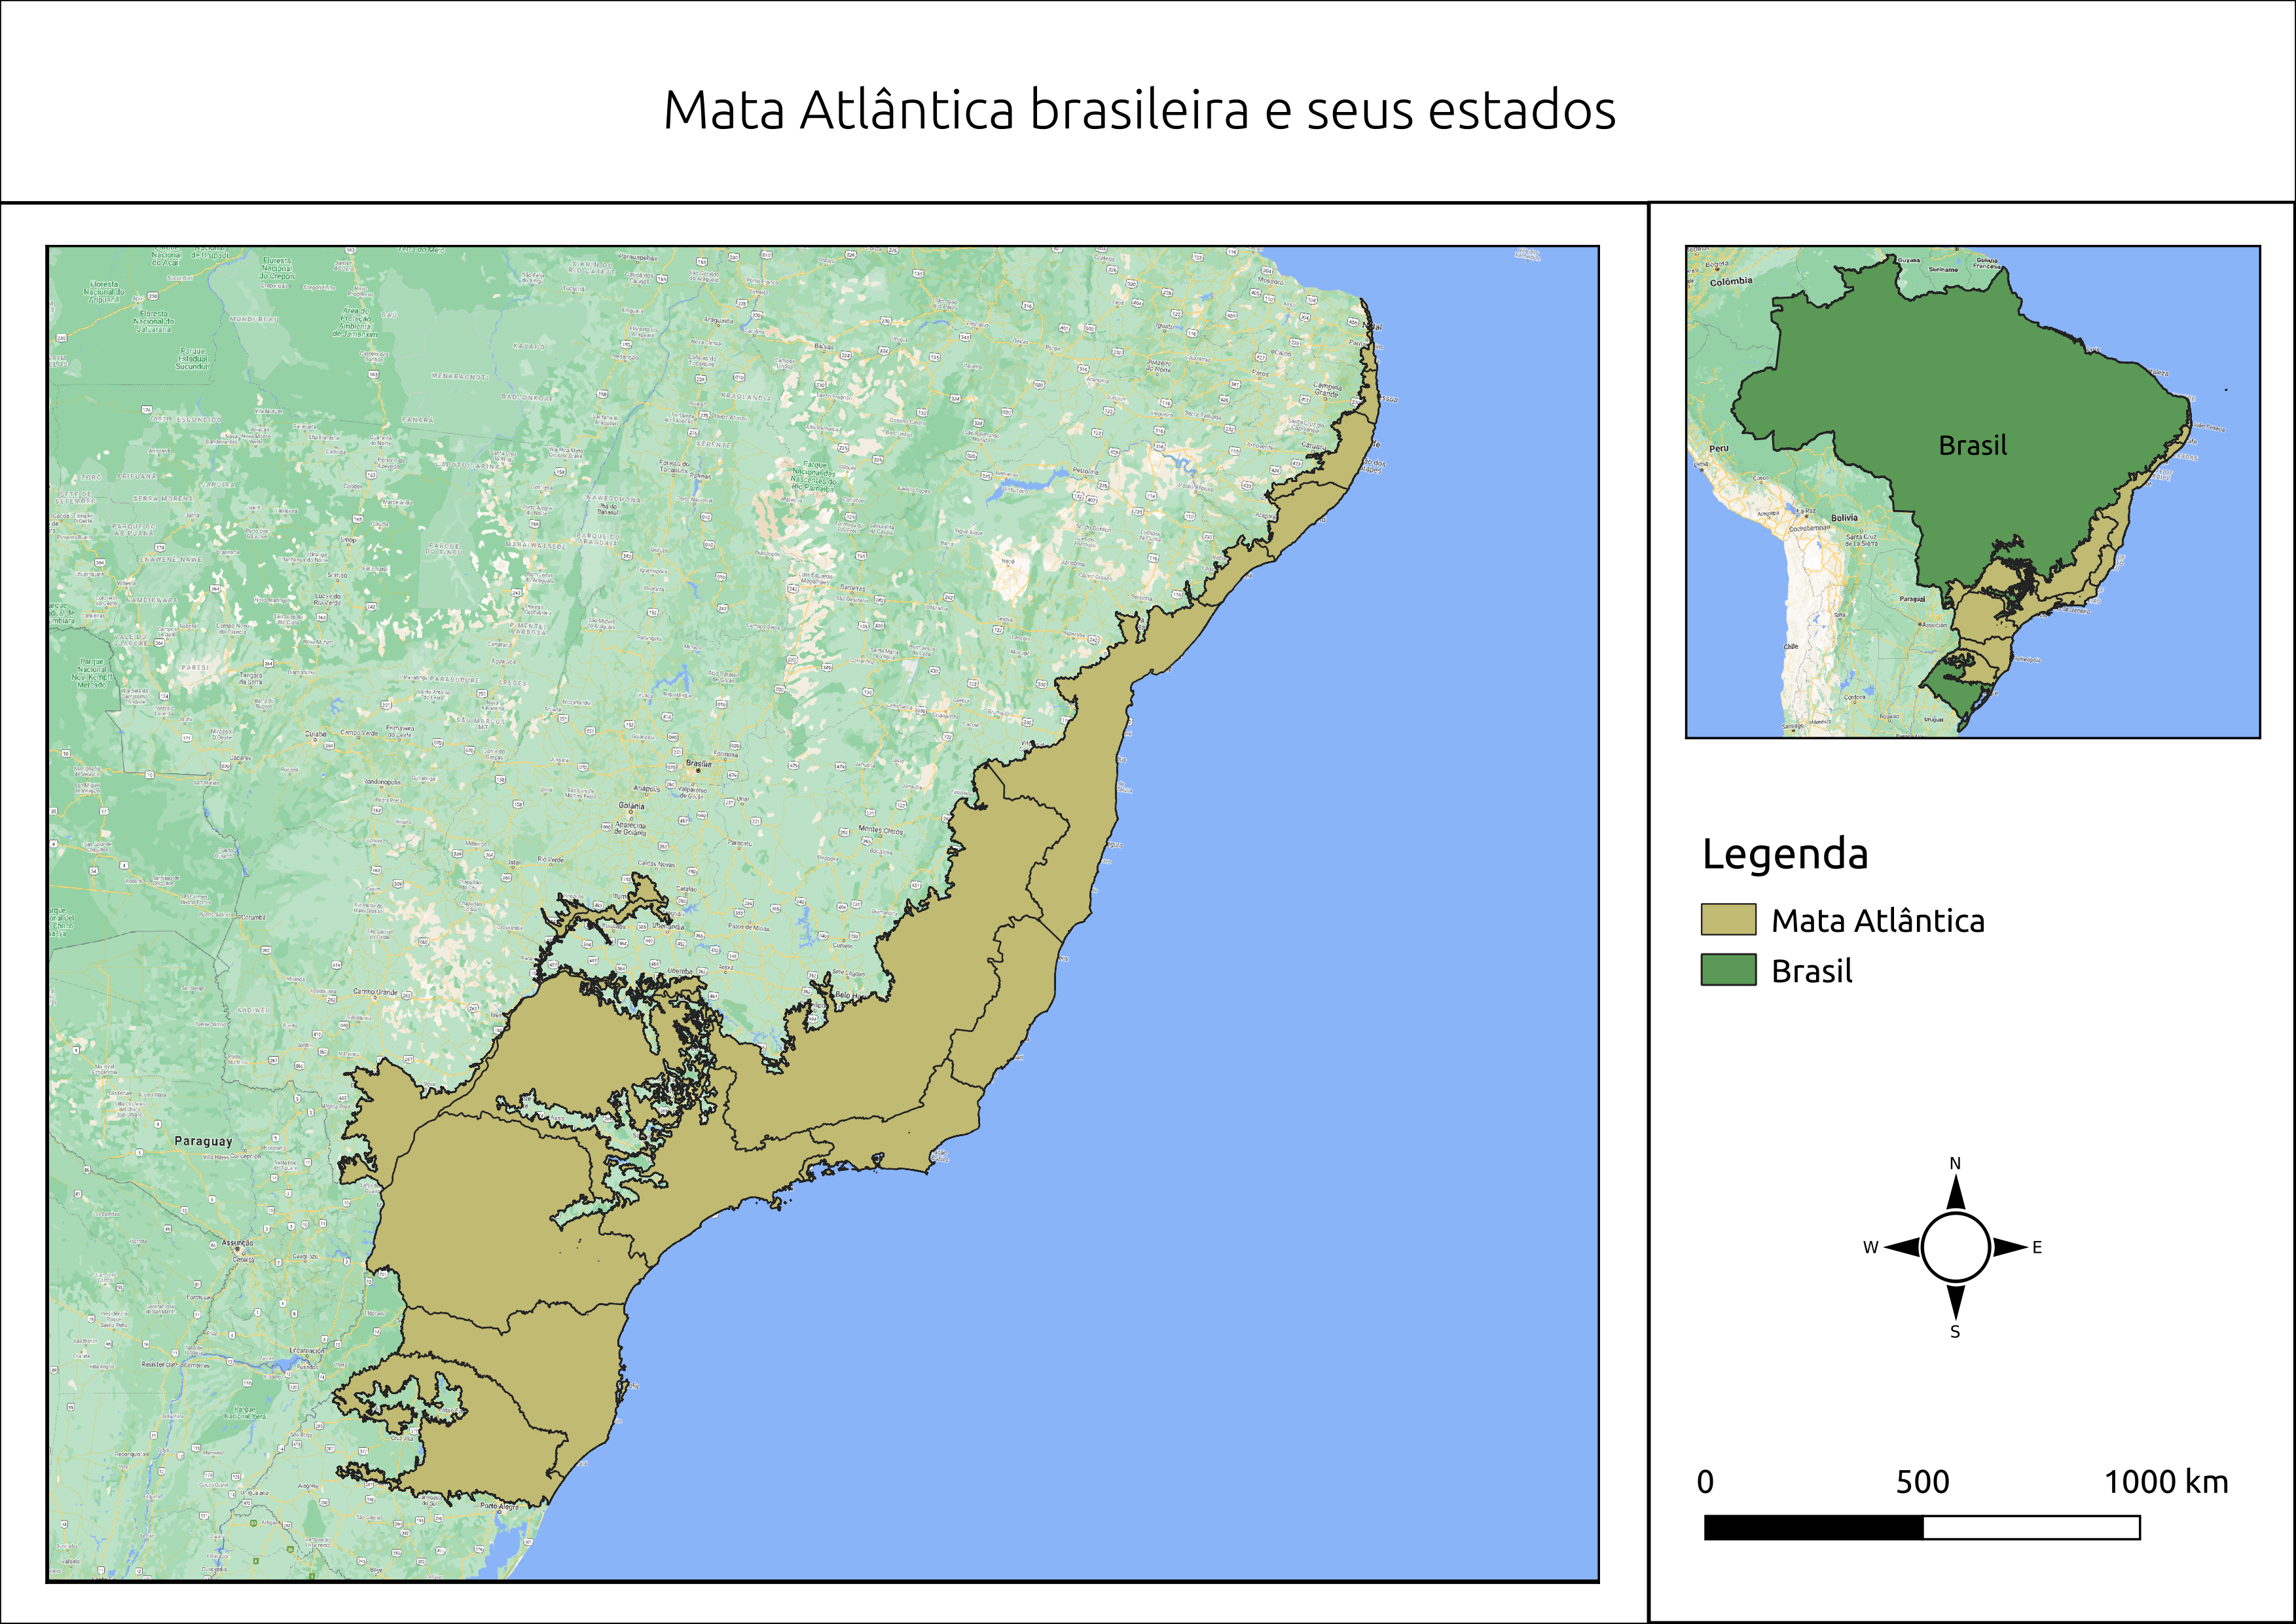
\includegraphics[scale=.5]{images/mata_atlantica.png}
    \caption{Área de Estudo - Mata Atlântica brasileira}
    \label{fig:mata_atlantica}
\end{figure}

\newpage

\subsection{Questionamentos e objetivos da pesquisa}
Os questionamentos motivadores e objetivos da pesquisa foram:
\begin{itemize}
    \item Como um algoritmo como o Landtrendr, inicialmente desenvolvido e utilizado para detecção de mudanças em ambientes de floresta temperada poderia ser utilizado para identificar com alta precisão mudanças ocorridas em uma paisagem complexa como a presente na Mata Atlântica brasileira?
    
    \item O aplicação da metodologia consegue boa performance geral e/ou em diferentes fitofisionomias considerando a aplicação do algoritmo com um mesmo conjunto de parâmetros?
    
    \item Quais as áreas com maior quantidade de perda e ganho de floresta?
    
    \item Como as unidades de preservação existentes da Mata Atlântica se comportaram ao longo dos anos? (ex. Parque Nacional da Serra da Bocaina, Parque Nacional da Serra dos Órgãos, etc)
    
    \item Como os estados e municípios se comportaram ao longo da série temporal? Quais deles ganharam mais do que perderam floresta?
    
    \item Quais os anos com maior quantidade de perda e ganho de floresta?
    
    \item Quais as áreas com maior taxa de mudança tanto para perda como ganho de vegetação? 
    
    \item Qual a idade das florestas secundárias do bioma? 
\end{itemize}

\subsection{Objetivos Específicos}
\begin{itemize}
    \item Definição do período, seleção das imagens e criação da composição da série temporal Landsat a ser utilizada;
    
    \item Compatibilização das imagens utilizadas de acordo com características geométricas e radiométricas com o intuito de evitar possíveis ruídos;
    
    \item Definição dos parâmetros e do índice espectral para a execução do processo de segmentação temporal utilizando o algoritmo Landtrendr;
    
    \item Desenvolvimento do código na plataforma Google Earth Engine para a execução do algoritmo em todas as cenas que englobam o bioma da Mata Atlântica brasileira;
    
    \item Mapeamento das trajetórias florestais compatível com a escala 1:100.000 através da criação de mapas de detecção de magnitude, ano de início da mudança, duração e taxa de mudança;
    
    \item Conversão dos dados matriciais gerados em dados vetoriais com intuito de identificar áreas com maior nível de ocorrência de perdas e ganhos de acordo com divisões políticas e geoecológicas;
    
    \item Mapeamento da idade da floresta secundária;
    
    \item Avaliação da acurácia dos produtos gerados. Avaliar o desempenho do algoritmo em ambientes de florestas tropicais com alto nível de complexidade ecológica.
\end{itemize}
\newpage

\section{Perspectivas sobre a Utilização de Algoritmos para o Processamento de Séries Temporais no Estudo de Distúrbios Florestais}

\subsection{Introdução}

\hspace{13pt} A incorporação do tempo como variável chave de estudos geográficos, principalmente os pautados na análise sistêmica da paisagem, se deu de forma bastante limitada principalmente pela dificuldade de acesso a séries históricas confiáveis, assim como pela dificuldade de manipulação das mesmas quase sempre através de um ambiente computacional também limitado.

Com o aumento significativo do uso da internet e da capacidade de hardware das últimas décadas, a utilização de métodos computacionais na análise de dados científicos se tornaram cada vez mais presentes com uma maior possibilidade de acesso não só a grandes bases de dados como também a ambientes computacionais de alto desempenho. Essa realidade passou a ser possível para um público que antes dependia quase que exclusivamente das estruturas disponíveis mais próximas e imediatas. Isso representa uma mudança significativa para pesquisadores de países onde o acesso as estruturas científicas quase sempre se dão de forma mais limitada. Consequentemente, isso se traduz na possibilidades de estudos não só mais detalhados e estruturados como também de pesquisas que abordem outras escalas de análise, o que por sua vez possibilita uma maior relevância científica internacional e maior reprodutibilidade dos estudos \citep{ArribasBel2018}.

A aplicação de técnicas de análise de séries temporais para o monitoramento espaço-temporal da paisagem tem surgido com maior força nos últimos anos como consequência dessa evolução histórica. A aplicação dessas técnicas é da mais diversa possível, vindo inicialmente quase que exclusivamente dos estudos econométricos e de poucas outras áreas científicas para a sua massificação em muitas outras áreas. Uma delas, e que será abordada neste trabalho é a utilização de técnicas de análise de séries temporais em imagens digitais orbitais com o intuito do monitoramento de áreas naturais florestadas, principalmente na detecção de distúrbios florestais. Esse tipo de aplicação vem ganhando força não só pelo entendimento das mudanças da paisagem e suas dinâmicas, como também pela preocupação com o monitoramento do desmatamento, monitoramento de projetos de restauração e também no acompanhamento de processos de regeneração natural que acontecem na paisagem. O monitoramento do uso do solo nunca teve tanta importância como hoje devido ao maior entendimento e comprometimento internacional em relação as variáveis influenciadoras do processo da mudanças climáticas através de tratados e acordos de estimulo à conservação e restauração de áreas naturais \citep{ALMEIDA201934}, entendendo ainda o protagonismo da análise espacial e do monitoramento por satélites como ferramenta essencial neste processo \citep{WHITE2019}. 

Políticas de REDD+, assim como vários esforços de cooperação internacional como os propostos pelo Bonn Challenge e os Aichi Targets deficidos pela CDB (\textit{Convention on Biological Diversity}), tem como ferramenta principal a incorporação de técnicas de sensoriamento remoto para o monitoramento do cumprimento dos objetivos, sendo então diretamente vinculados ao entendimento do comportamento da paisagem no tempo \citep{BOS2019295, CROUZEILLES2019}. Estudos mais recentes vem demonstrando que os processos de degradação em florestas tropicais tem impacto similar ou até mesmo maior em relação as emissões de carbono que o desmatamento das mesmas \citep{Harris1573, Houghton2012, Grace2014}. É importante notar aqui que a utilização do termo distúrbio é diferente do de degradação. Enquanto distúrbio está associado a um único evento que pode ser tanto natural como antrópico, degradação se associa a um processo temporalmente maior de perda de biomassa e a um tipo de influência necessariamente antrópica se considerarmos a definição do IPCC (\textit{Intergovernmental Panel on Climate Change}) ou não necessariamente antrópica caso se considere a definição da FAO (\textit{Food and Agriculture Organization of the United Nations}) \citep{Hirschmugl2017}. 

Além disso, outros estudos demonstram que as florestas tropicais tem sofrido mais pressões do que as temperadas. Um terço das florestas tropicais já foram perdidas para o desmatamento, e da área restante, 46\% da área está fragmentada, 30\% degradada e apenas 24\% ainda permanece em estado mais preservado. Sabendo disso, fica ainda mais clara a necessidade de entender quais as melhores técnicas que podem ser utilizadas para o monitoramento destes processos \citep{Hirschmugl2017}. 

O momento político e histórico de acordo com a perspectiva da preservação do meio ambiente na qual estamos inseridos necessita ainda mais que as pesquisas de monitoramento de distúrbios sejam feitos de forma cada vez mais transparente e acessíveis a todos para que processos de degradação sejam detectados a tempo. Com isso, é importante entendermos quais tecnologias estão disponíveis e quais as possibilidades de monitoramento são possíveis, tendo como objetivo principal entender não só suas potencialidades como suas limitações. 

Sendo assim, este trabalho tem como objetivo a apresentação e análise das características dos principais algoritmos de detecção de distúrbios, principalmente os especializados na detecção de mudanças em áreas florestadas, seja na perda como no ganho de biomassa.


\subsection{Breve Histórico}

\hspace{13pt} Estudos espaço temporais com o objetivo de detecção de mudanças não são novos na área do sensoriamento remoto. A tradicional análise bi-temporal de dados previamente classificados ainda é presente em muitos estudos atuais. No entanto, esse tipo de estudo tende a conter um número maior de erros, já que quanto maior o número de imagens analisadas, maior a quantidade de mapas com erros de classificação associados que serão levados em consideração. De qualquer forma, estes tipos de estudos tendem a ser o que possuem menor requisito de poder computacional, já que necessitam apenas de operações simples entre álgebra de bandas.

Com o tempo, o maior poder computacional disponível não só para o processamento como para o armazenamento de dados possibilitou que outras técnicas mais elaboradas pudessem ser implementadas, onde ao invés de apenas algumas imagens serem consideradas, todas as imagens da série temporal são levadas em consideração. Isso possibilitou também que muitas técnicas de análise de séries temporais tipicamente aplicadas principalmente na área de econometria pudessem ser utilizadas em estudos geoespaciais.

O processamento de imagens de satélite que historicamente sempre foi feito através do processamento de pixels individuais, passou a partir da década de 00 a ser feita em muitos casos através do delimitação de objetos com a popularização das imagens de alta-resolução espacial e consequentemente das técnicas de GEOBIA (\textit{Geographic Object-Based Image Analysis}). As análises pixel à pixel que pareciam estar cada vez mais em desuso, acabaram ressuscitando nos últimos anos devido a capacidade de processamento de séries temporais densas. A densidade da série é um ponto chave para esse retorno, já que para que a análise temporal seja bem sucedida e para que os algoritmos aplicados possam entender ainda melhor os processos ocorridos no tempo, é necessário que os dados utilizados tenham resolução temporal condizente com o que se quer detectar. No caso da utilização de imagens de satélite isso se torna um limitador importante, já que a disponibilidade de satélites imageadores historicamente nunca foi alta e tem custo extremamente elevado quando comparado a outros tipos de sensores. Outro problema é que os satélites possuem um tempo de revisita que em muitos casos não possibilitam que uma série mais densa possa ser estruturada. 
%\par
Além disso, problemas como a presença de nuvens, assim como ruídos na própria imagem e a heterogeneidade da distribuição solar no planeta e sua interação com o relevo dificultam ainda mais esse processo ao criar sombras. No entanto, com o tempo, outros satélites foram sendo desenvolvidos e propositalmente pensados com o objetivo de incorporar as séries de imagens já existentes derivadas de projetos antigos com os recém lançados. Um exemplo disso foi o lançamento da série Sentinel 2 (A e B) pela Agência Espacial Europeia com uma resolução espectral e espacial similar as encontradas na série Landsat, o que possibilita uma fusão entre imagens de satélites diferentes com o objetivo de aumentar a densidade de imagens. Com isso, tanto a disponibilidade de dados como a resolução temporal dos satélites ganharam nova relevância. A disponibilização de imagens de forma gratuita, assim como a preocupação com a manutenção de séries históricas e o desenvolvimento de constelações que diminuam a resolução temporal acabaram possibilitando esse retorno do pixel como chave analítica central no sensoriamento remoto.


\subsection{Técnicas e Algoritmos para a Análise Temporal de Áreas Florestadas}
\hspace{13pt} Analisar áreas florestadas sob uma perspectiva temporal possibilita a identificação de processos e padrões que uma simples caracterização espectral mais tradicional não é possível de identificar devido a limitações ligadas a resolução espacial, radiométrica e espectral. Sendo assim, ao incluir a dimensão temporal, é possível entender dinâmicas como a supressão da floresta em um dado momento, assim como também os distúrbios naturais e degradações de origem antrópica ao longo do tempo.
A degradação associada ao desmatamento e posterior uso agrícola da terra, seguido do abandono e consequente retorno da vegetação através de processos de regeneração natural, ou então um processo de degradação mais lento, como a extração seletiva de madeira, são exemplos de mudanças no uso e cobertura da terra que só podem ser compreendidos através de técnicas como as que serão mostradas neste trabalho. 

Técnicas de detecção de mudança possuem uma longa história na área de sensoriamento remoto. Desde as primeiras aplicações utilizando sensores TM do satélite Landsat 5 na década de 1980 e 1990, muitos estudos foram feitos. Inicialmente os estudos visavam majoritariamente na aplicação de técnicas mais tradicionais como o mapeamento das áreas de interesse utilizando técnicas tradicionais de classificação de imagens tanto de forma supervisionada como não supervisionada e posterior cálculo da diferença entre as duas ou mais imagens. Neste caso, somente métricas como o ganho e perda de área e sua consequente espacialização poderiam ser extraídas e visualizadas. No entanto, com o aumento do poder computacional e consequente amadurecimento das técnicas, softwares e bibliotecas disponíveis, o processamento de dados multi-temporais passaram a ser entendidos em sua totalidade. Ou seja, com a aplicação de técnicas menos reducionistas. O que isso significa na prática é que a análise de mudanças de áreas de floresta passou a ser feita através da manipulação tanto da criação de composições anuais, assim como intra-anuais e também da análise de toda a série temporal sem maiores cortes.

Para o processamento de séries temporais utilizando imagens de satélite é necessário se preocupar também com o pré processamento das mesmas para que a aplicação do algoritmo, seja ele qual for, não influencie o resultado final com ruídos derivados de falta de calibração geométrica entre as imagens de diferentes datas, assim como a variação radiométrica, além da presença de possíveis sombras. Para isso, é necessário utilizar técnicas de pré-processamento como a ortorretificação e a correção radiométrica (atmosférica) das imagens. Dependendo do satélite utilizado é possível utilizar métodos implementados pela própria agência distribuidora, o que é bastante recomendado. No caso da correção geométrica das imagens, muitas já são disponibilizadas após serem tratadas automaticamente por método de correção subpixel \citep{Gutjahr2014}. Já para a correção radiométrica existem dois tipos: as calibração absoluta e a relativa. A absoluta faz a calibração transformando os valores digitais em valores físicos de superfície e aplicando algoritmos como o 6S \citep{Sagan2004}, já a calibração relativa utiliza uma imagem de referência como base e aproxima os valores do resto da série de acordo com a imagem base. Trabalhos comparando os dois métodos já foram desenvolvidos utilizando imagens Landsat e apresentam resultados similares \citep{Chen2010}. Produtos da série Landsat ainda possuem métodos internos de correção além de máscaras para a filtragem de nuvens, sombras e outras características das imagens \citep{ZHU2015269, ZHU201283, Huang2010}, o que facilita bastante a etapa de pré-processamento.

Alguns algoritmos foram sendo desenvolvidos ao longo dos últimos anos com o objetivo de lidar melhor com essas séries. Um dos mais tradicionais é o BFAST \sloppy  \citep{VERBESSELT2010106, VERBESSELT20102970, VERBESSELT201298} que possui uma versão visando dados espaciais denominada bfastSpatial \citep{bfastSpatial}. As duas ferramentas possuem o mesmo algoritmo de detecção, mas a versão espacial se diferencia por conta de uma série de funções voltadas para facilitar o pré-processamento dos dados com o intuito de construir inicialmente a série temporal. A construção das séries temporais em ambiente offline sem ajuda de ferramentas mais modernas é, de fato, bastante trabalhosa e contém muitas etapas necessárias para que a análise final possa ser feita sem maiores problemas e sem a geração de ruídos por conta de dados de entrada problemáticos. É importante notar também que as duas ferramentas, diferentemente de outros algoritmos que serão analisados neste trabalho, não são voltados exclusivamente para a detecção de distúrbios em ambientes florestais,  mas sim em basicamente qualquer outro tipo de uso. No entanto, o uso das duas ferramentas em ambientes florestais é provavelmente o mais comum entre os trabalhos existentes. 

O BFAST tem como ideia geral analisar a série temporal de imagens analisando os valores pixel à pixel e detectando quebras (\textit{breakpoints}) de pixels que tenham valor discrepante do valor médio esperado. É possível detectar mais de uma quebra em uma mesma série de pixels, o que é interessante principalmente para análise de usos agrícolas, assim como quando comparados a áreas florestais. O algoritmo ainda pode ser utilizado em objetos, como apresentado por Siti Latifah \citep{LATIFAH2016}, onde a integração com técnicas de GEOBIA apresentou ótimos resultados. Este resultado demonstra ainda um novo potencial a ser explorado, onde a integração de dois paradigmas (pixel/objeto) através do processamento de séries temporais pode trazer novas formas de análise e até mesmo a implementação de novos algoritmos.

Já outros trabalhos utilizando o BFAST demonstraram a capacidade do mesmo na detecção de quebras para a caracterização de distúrbios cíclicos em florestas com o objetivo de explicar mudanças estruturais que acabam influenciando diretamente na qualidade da floresta presente e não só na sua simples presença ou não presença \citep{JAKOVAC2017, DUTRIEUX2016112}.

Mais recentemente, o BFAST passou por um processo de reimplementação, deixando a linguagem R de lado como em sua versão original e sendo totalmente reprogramado utilizando a linguagem Python. Essa mudança se deu pela fato da nova versão possuir uma integração direta com a biblioteca de processamento paralelo OpenCL, o que garantiu uma diminuição no tempo total de processamento em duas ordens de grandeza \citep{Gieseke2020}. Por utilizar um padrão aberto de paralelismo, a nova implementação possui a capacidade de poder se beneficiar do paralelismo independente do tipo e do fabricante do hardware, podendo ser paralelizado tanto na CPU (Intel/AMD) quando na GPU (Nvidia, AMD, Intel).

Além do BFAST, outras implementações computacionais foram desenvolvidas com o objetivo de analisar séries temporais para detecção de padrões em tipos variados de uso do solo. Este é o caso do Timesat \citep{Jnsson2004TIMESATA}. O Timesat, apesar de ter a aplicação mais voltada para a caracterização de tipos de culturas agrícolas através da interpretação da série, também possui uso na caracterização de tipos e também de distúrbios em florestas \citep{Wenbo2017}. O Timesat ainda possui diversas ferramentas internas para o tratamento de ruídos, tratamento de dados faltantes e composição de séries sazonais utilizando algoritmos como o Savitzky-Golay \citep{Savitzky1964}.

Ao aprofundarmos mais, para além das técnicas mais tradicionais, podemos entender que esses algoritmos apresentados, assim como muitos outros existentes se diferenciam entre si. Além disso, alguns deles acabam sendo desenvolvidos como algoritmos especialistas na aplicação de detecção de distúrbios em florestas, ao contrário dos algoritmos já citados. Esses novos métodos de análise ainda podem ser categorizados em quatro sub-categorias: algoritmos baseados na detecção de mudanças baseados em limiares, os baseados em ajude de curvas, os baseados no ajude de trajetórias e os baseados na segmentação de trajetórias \citep{Banskota2014, Hirschmugl2017}.

\subsection{Detecção de Mudanças Baseado em Limiares}
\hspace{13pt} Os métodos de detecção baseados em limiares funcionam buscando a diferenciação de áreas de floresta e não floresta, e posteriormente separando áreas de floresta "intacta" das que sofreram algum tipo de distúrbio ou processo de degradação. A ideia é utilizar uma série temporal previamente tratada formadas tanto puramente por índices de vegetação, como pela integração de diversas bandas espectrais e bandas sintéticas derivadas de estatísticas da própria série. Esses métodos possuem um grande potencial e aplicação, mas ao mesmo tempo tem como ponto negativo a necessidade da delimitação empírica de limiares, o que dificulta bastante a replicabilidade dos trabalhos.

\subsection{Detecção de Mudanças Baseado no Ajuste de Curvas}
\hspace{13pt} A utilização de métodos baseados no ajuste de curvas em áreas florestadas tem como objetivo entender o comportamento espectral primeiramente aplicando uma linha de regressão, onde dependendo da inclinação da mesma é possível detectar a presença ou ausência de mudanças significativas. Além disso, o sinal da inclinação determina também o ganho ou perda de biomassa. O lado negativo desse método é a necessidade da suposição de uma certa normalidade entre os dados de entrada, o que em sensoriamento remoto é quase sempre muito difícil de se obter. Isso já tende a limitar a aplicação de métodos como esse a sensores com menor resolução temporal como os presente no projeto MODIS (\textit{Moderate-Resolution Imaging Spectroradiometer}), ou então de composições muito bem estruturadas de sensores como o Landsat. A utilização desse método pode ser exemplificado pelo trabalho desenvolvido no bioma amazônico utilizando imagens MODIS onde é demonstrado a relação entre o corte seletivo e a mudança da resposta fenológica da vegetação na região ao longo do tempo \citep{KOLTUNOV20092431}.

\subsection{Detecção de Mudanças Baseado no Ajuste de Trajetórias}
\hspace{13pt} As técnicas de ajuste de trajetórias se diferenciam dos anteriores por analisarem as mudanças a partir de trajetórias idealizadas. Através da aplicação de métodos comparativos (ajuste) entre a série estudada com a de referência, seja através do cálculo da distância euclidiana como pela utilização de métodos mais complexos como o DTW (\textit{Dynamic Time Warping}) \citep{VELICHKO1970223, SakoeChiba71, Berndt1994} e sua versão para a classificação de uso do solo, o TWDTW (\textit{Time-Weighted Dynamic Time Warping}) \citep{Maus2016, Maus2019}, o ajuste de trajetórias funciona como um método de análise supervisionado já que depende de amostras de "treino" para a obtenção de resultados satisfatórios.

Este tipo de algoritmo, devido a sua natureza de carácter supervisionado, tem sido utilizado principalmente em estudos aplicados na tipificação de culturas agrícolas, onde a diferenciação dos alvos só pode ser feita utilizando conhecimentos relativos ao comportamento espectral do alvo no tempo. Este tipo de algoritmo necessita de uma densidade de imagens maior que as outras técnicas, já que é necessário o maior grau possível de precisão na série para encaixar e detectar as características entre as duas séries. Para este tipo de aplicação são utilizados normalmente imagens derivadas do sensor MODIS, devido a sua resolução temporal e as suas aplicações na caracterização do comportamento espectral de grandes áreas agrícolas, onde a resolução espacial do satélite (250m) não impede a análise de ser realizada. É possível utilizar imagens Landsat com este método, mas é necessário acumular uma grande densidade de imagens através da fusão do histórico de vários sensores e/ou trabalhando com área de interseção entre path/row diferentes, o que limita sua aplicação \citep{Bendini2016}. Além dessas limitações, outros desafios vem sendo enfrentados em relação a dificuldade de detecção de distúrbios pontuais de corte seletivo e posterior regeneração natural do local, já que amostras muito bem definidas para este tipo de distúrbio precisam ser coletadas. No entanto, exemplos de aplicação em florestas tropicais são presentes \citep{Hirschmugl2013, KENNEDY2007370}.


\subsection{Detecção de Mudanças Baseado na Segmentação de Trajetórias}
\hspace{13pt} O método de segmentação de trajetórias pode ser exemplificado pelo algoritmo Landtrendr \citep{KENNEDY20102897, KENNEDY2012117}, que funciona dividindo a série temporal em segmentos para posterior estudo. Este tipo de abordagem favorece estudos onde em uma mesma série (pixel) é possível entender vários processos. É possível não só a detecção de distúrbios em períodos de tempo curtos (provável evento de desmatamento), assim como na detecção de distúrbios de longo prazo (possível processo de degradação/corte seletivo), como processos de regeneração com longa duração (regeneração natural) e de curto prazo (floresta plantada e projetos de reflorestamento). Esses segmentos são realizados a partir da estipulação de vértices durante a série. Os vértices representam os pontos da série onde houve algum tipo de mudança na qual o algoritmo considerou relevante. A escolha da relevância para a criação de um vértice (quebra) é feita de acordo com regras pré-definidas pelo usuário. Outra vantagem desse método é a possibilidade de análise sem a necessidade de amostras de eventos exemplo como no caso dos algoritmos de ajustes de trajetórias.
No entanto, o método de segmentação de trajetórias também possui suas desvantagens. A principal é que o algoritmo desconsidera efeitos sazonais da vegetação. Além disso, é um método que apesar de possuir alguns trabalhos aplicando suas técnicas em florestas temperadas \citep{PFLUGMACHER2012146, Griffiths2015}, ainda possui poucos estudos em áreas tropicais.

\subsection{Exemplos de Ferramentas e suas Características}
\hspace{13pt} Além do BFAST e de outros algoritmos/softwares apresentados previamente, podemos listar brevemente alguns outros algoritmos de detecção automática de mudanças. É importante notar que alguns desses na verdade não realizam exatamente o trabalho de detecção da mudança, mas sim mais um processo de predição dessas mudanças, já que trabalham a partir de técnicas de regressão. Algumas características e particularidades de cada algoritmo também serão apresentadas. Todos foram desenvolvidos nos últimos anos e representam grande parte dos métodos de detecção automática de distúrbios presentes na literatura recente. São eles: 

\begin{itemize}
  \item \textbf{CCDC} - \textit{Continuous Change Detection and Classification} \citep{ZHU2014152} - O CCDC apresenta funções de análise de séries temporais utilizando não composições anuais ou intra-anuais, mas sim toda a série de imagens de entrada, o que o difere da maioria dos algoritmos exemplificados aqui. O CCDC funciona apenas com imagens sem a presença de nuvens e sombra e busca encontrar padrões de sazonalidade, tendências e quebras na série. Uma característica interessante do CCDC é que o algoritmo é capaz de gerar imagens "sintéticas" para qualquer data presente na série de entrada \citep{ZHU201567}. Estas imagens sintéticas geradas são utilizadas obrigatoriamente como dado de entrada por algoritmos como o MIICA e o ITRA e também podem ser utilizadas opcionalmente por algoritmos como o Landtrendr e o VCT, ao invés de utilizar as imagens originais com valores de reflectância da superfície. O CCDC é utilizado para a detecção de eventos de grande magnitude, sendo então limitado na detecção de processos de degradação, por exemplo. No entanto, pode ser utilizado na detecção de mudanças de vários tipos de uso do solo e não somente na deteccão de distúrbios florestais.
  
  \item \textbf{COLD} - \textit{Continuous Monitoring of Land Disturbance} \citep{Cohen2020} - O COLD é baseado no CCDC com o objetivo de melhorar a detecção de distúrbios florestais. Diferente do CCDC que detecta mudanças baseadas em eventos de grande diferença espectral, o COLD possui a capacidade de detecção de mudanças mais sutis, o que lhe garante suprir essa deficiência presente no CCDC.
  
  \item \textbf{LandTrendr} \citep{KENNEDY20102897, KENNEDY2012117} - O Landtrendr, desenvolvido pelo Environmental Monitoring, Analysis and Process Recognition Lab da Universidade de Oregon, também trabalha tanto com composições de imagens com valores de reflectância da superfície como com imagens sintéticas geradas pelo CCDC. O algoritmo necessita que as imagens não possuam interferência de nuvens e sombras e gera seus dados de saída através da aplicação da técnica de segmentação de trajetórias. O Landtrendr pode gerar saídas como métricas tanto para distúrbios de perda como de ganho, além de detectar se as mudança ocorreram de forma lenta ou rápida, possibilitando também o cálculo da duração dos eventos segmentados previamente gerando não só dados contínuos como a magnitude, assim como dados discretos como a durança e o ano da detecção. É certamente um dos algoritmos com maior quantidade de informação gerada por rodada, o que facilita em muito sua utilização. Outra vantagem do Landtrendr é que apesar de ter sido implementado inicialmente utilizando a linguagem de programação proprietária IDL em um ambiente bastante complicado de manuseio através do software ENVI, foi recentemente implementado diretamente na plataforma online Google Earth Engine \citep{GORELICK201718}, o que veio a facilitar e muito sua utilização pela comunidade \citep{Kennedy2018}. A conversa do algoritmo para a plataforma online do Google possibilitou ainda que o tempo de processamento do mesmo fosse reduzido significativamente. No entanto, a plataforma restringe o processamento para no máximo a área equivalente de uma imagem Landsat por vez.
  
  \item \textbf{VCT} - \textit{Vegetation Change Tracker} \citep{Huang2010, THOMAS201119} - O VCT utiliza composições sem nuvem de imagens com valor de reflectância da superfície, ou de composições sintéticas geradas pelo algoritmo CCDC e extrai uma métrica de similaridade a áreas de floresta intacta. O algoritmo prediz os distúrbios detectando padrões que se afastam da métrica de similaridade.
  
  \item \textbf{EWMACD} - \textit{Exponentially Weighted Moving Average Change Detection} \citep{Brooks2014} - Este algoritmo foi desenvolvido com o objetivo de detectar apenas distúrbios florestais ao analisar o resíduo entre o pixel observado e os valores derivados de uma predição gerado por um processo de regressão harmônica \citep{Brooks2012}. Além disso, tem como característica, assim como o CCDC, utilizar todas as imagens de entrada ao invés de composições. Também possui uma série de funções e parâmetros para a detecção de mudanças de pouca magnitude e de longo prazo, apresentando bons resultados na detecção de processos de degradação.
  
  \item \textbf{VerDET} - \textit{Vegetation Regeneration and Disturbance Estimates through Time} \citep{Hughes2017} - O VerDET funciona através da entrada de composições anuais sem nuvem com valores de reflectância de superfície que são segmentadas se baseando em técnicas de regressão utilizando redes neurais artificiais. Para cada pixel o slope é calculado e são posteriormente interpretados como áreas de distúrbio, estabilidade e regeneração, além de apresentar as magnitudes para a interpretação e classificação entre eventos rápidos ou lentos. Assim como o EWMACD, o VerDET também foi desenvolvido para trabalhar apenas com detecção de distúrbios em florestas.
  
  \item \textbf{MIICA} - \textit{Multi-index Integrated Change Analysis} \citep{JIN2013159} - Este algoritmo utiliza a composição de imagens sintéticas como entrada e tem como característica realizar sua análise baseado em limiares em invervalos bi-anuais. O MIICA analisa as mudanças espectrais de magnitude baseado nesses limiares utilizando quatro índices diferentes (NBR - \textit{Normalized Burn Ratio}, NDVI - \textit{Normalized Difference Vegetation Index}, \textit{Change Vector} e o \textit{Relative Change Vector Maximum}). Pode detectar mudanças relacionadas ao ganho e perda de biomassa e também a cenários de não mudança. É voltado para a detecão de grande magnitude e pode ser utilizado para a detecção de mudança em vários tipos de uso do solo.
  
  \item \textbf{ITRA} - \textit{Image Trends from Regression Analysis} \citep{VOGELMANN201292} É outro algoritmo que utiliza composições anuais sem nuvem geradas sinteticamente pelo CCDC. O ITRA ainda divide a série em três períodos e compara as mesmas com um modelo de regressão linear. É um algoritmo que tem como ênfase a detecção de distúrbios de longo período tanto em florestas como em áreas com vegetação arbustiva. Devido a sua característica de poder identificar mudanças de diferentes magnitudes, o ITRA pode ser utilizado detecção não só de distúrbios em florestas como também em outros tipos de vegetação.
  
  \item \textbf{Shapes-NBR} \citep{Meyer2013, Moisen2016} Como o nome já demonstra, este algoritmo funciona através da composição de uma série temporal de índices NBR, o que difere de sua aplicação original, onde era utilizado apenas como um preditor de mudanças em áreas florestadas e chamado apenas de Shape \citep{SCHROEDER2017230}. O algoritmo funciona para cada pixel aplicando um algoritmo de regressão aditiva semi-paramétrico fornecendo uma trajetória suavizada restrita para se comportar de uma maneira ecologicamente sensíveis. Assim como o Landtrendr, este também gera resultados de acordo com as formas encontradas como o ano da detecção, magnitude da mudança, valores prévios à mudança e posteriores a mesma e taxas de crescimento ou recuperação.
  
\end{itemize}

\subsection{Validação de Séries Temporais}
\hspace{13pt} O processo de validação de séries temporais se difere dos adotados em estudos de mapeamento de apenas uma ou poucas datas de estudo. Normalmente as amostras de validação são extraídas de apenas uma única data e comparada ao resultado obtido, no entanto, no caso do processamento de séries temporais, muitas datas ou até mesmo toda uma série de imagens são utilizadas como dado de entrada para os algoritmos preditores. Sendo assim, o método tradicional perde sua validade. É necessário analisar toda a série de imagens utilizadas para entender os momentos de possível quebra e consequente detecção do distúrbio para podermos validar com maior clareza. Principalmente em situações onde houve distúrbios florestais que aconteceram em um determinado momento histórico e que posteriormente iniciaram um processo de regeneração natural ou então uma mudança para um terceiro uso do solo. Quanto maior a quantidade de tipos de mudança ocorridos durante o tempo analisado, maior a complexidade e consequente necessidade de utilização de métodos de validação apropriados.

Um dos métodos mais utilizados atualmente na validação de séries temporais, independentemente do algoritmo que foi utilizado para a detecção das mudanças é o TimeSync \citep{COHEN20102911}.O TimeSync possui versão offline utilizando uma interface gráfica onde é possível visualizar não somente uma imagem/data, mas toda a série temporal tanto em forma de gráfico como com miniaturas de imagens referentes a área próxima na qual o pixel está sendo analisado. Além disso, após a implementação do algoritmo Landtrendr na plataforma Google Earth Engine, é possível exportar os dados para validação diretamente da plataforma online.  O TimeSync funciona recebendo uma lista de coordenadas na qual ele utiliza para exportar pequenas imagens com um buffer da coordenada analisada para cada ano da série. O software utiliza uma interface gráfica para apresentar uma imagem por ano para cada coordenada e assim possibilitar que o pesquisador faça a validação visual de cada local ao longo do tempo. 

\subsection{Novas Perspectivas}
\hspace{13pt} Com a possibilidade de uso de diversos algoritmos e tipos de análise disponíveis, a escolha por um único método de análise pode ser problemática. Trabalhos desenvolvidos com o objetivo de comparação entre os algoritmos também podem ser problemáticos já que muitos dos algoritmos não se propõe exatamente ao mesmo tipo de análise. No entanto, é possível encontrar trabalhos que vem trabalhando uma integração dos mesmos com o objetivo de encontrar o melhor resultado possível. O trabalho proposto por \citep{HEALEY2018717} buscou integrar todos os oito algoritmos citados neste trabalho junto a outros dados de entrada como o próprio conjunto de imagens com valores de reflectância da superfície, relevo e um mapa temático com os tipos de vegetação presente nas cenas. Todos os dados de entrada foram então processados e classificados utilizando uma implementação do Random Forest \citep{Breiman2001}. Vários resultados foram gerados utilizando todos os dados de entrada assim como variações de combinação entre eles: resultados utilizando somente imagens Landsat, utilizando somente o resultado da combinação de todos os oito algoritmos preditivos, todos os algoritmos combinado as imagens landsat, entre outros. O resultado que acabou representando a menor quantidade de erros foi justamente o que levou em consideração todos os dados de entrada possíveis.

Outro estudo ainda mais recente desenvolvido por \citep{BULLOCK2019111165} também buscou analisar distúrbios florestais integrando vários algoritmos apresentando ótimos resultados. Além disso, implementações feitas utilizando somente algoritmos com o Random Forest analisando séries temporais de imagens Landsat junto a camadas derivadas de estatísticas simples foram realizadas e também obtiveram resultados promissores \citep{WANG2019474}.
Estudos como os citados demonstram que apesar do bom resultado obtido individualmente, os algoritmos de detecção estudados possuem um potencial ainda maior de resultados ainda melhores quando integrados ou entre si e/ou utilizando técnicas híbridas. Além disso, não é possível dizer que um algoritmo ou técnica seja melhor que outra. Cada técnica apresenta pontos positivos e negativos dependendo do tipo de análise a ser realizada.

\subsection{Conclusão}
\hspace{13pt} Ao analisar as opções de algoritmos disponíveis entendendo melhor suas características positivas e negativas, assim como outras possibilidades de implementação das análises de séries temporais de forma integrada, podemos compreender melhor o potencial da pesquisa na área. O desenvolvimento de soluções de monitoramento de distúrbios e de processos de degradação assim como de regeneração, restauração e conservação de áreas de interesse tem alavancado ainda mais a aplicabilidade dos acordos nacionais e internacionais que são mais do que nunca necessários para criar pressões políticas e econômicas buscando resultados reais. Sendo assim, o revisão de conceitos e tecnologias apresentados neste trabalho espera ter contribuído para uma atualização da comunidade científica em relação ao tema abordado.
\newpage

\begin{titlepage}
    \centering
    \vspace*{\fill}

    \vspace*{0.5cm}
    
    \Large% \bfseries
    Capítulo 2

    \vspace*{1cm}

    \Large% \bfseries
    Uso do algoritmo Landtrendr em larga escala no contexto tropical: Um estudo de caso na Mata Atlântica entre os anos de 1985 e 2018

    \vspace*{5cm}

    % \large Eduardo Ribeiro Lacerda

    \vspace*{\fill}
\end{titlepage}

\section{Uso do algoritmo Landtrendr em larga escala no contexto tropical: Um estudo de caso na Mata Atlântica entre os anos de 1985 e 2018}

\begin{abstract}
    abstract
\end{abstract}

\subsection{Introdução}
\hspace{13pt} A disponibilização de forma gratuita de imagens Landsat ao longo dos anos possibilitou um aumento significativo no número de estudos em diversas áreas ao redor do mundo \citep{ZHU2019382, WULDER20122}. Já o surgimento recente de ferramentas de processamento paralelo na nuvem como o Google Earth Engine \citep{GORELICK201718} vem possibilitando agora uma ampliação tanto da área dos estudos quanto também na densidade de cenas, ou seja, na quantidade de imagens Landsat processadas para um único local, o que significa um maior desenvolvimento nas análises temporais.

A incorporação do tempo nas análises espaciais possibilita não só uma maior compreensão dos processos que ocorrem na paisagem como pode ser usado como subsídio para o gerenciamento de recursos e monitoramento de áreas de conservação ou projetos de restauração, estes cada vez mais importantes no contexto geopolítico atual devido principalmente aos efeitos crescentes das mudanças climáticas.

Com o intuito de possibilitar estas análises, algoritmos especializados passaram a ser desenvolvidos principalmente na última década. Podemos citar como exemplo o desenvolvimento de ferramentas como o CCDC \citep{ZHU2014152}, COLD \citep{Cohen2020}, VCT \citep{Huang2010, THOMAS201119} , VerDET \citep{Hughes2017}, EWMACD \citep{Brooks2014}, MIICA \citep{JIN2013159}, ITRA \citep{VOGELMANN201292}, Shapes-NBR \citep{Meyer2013, Moisen2016} e o Landtrendr \citep{KENNEDY20102897, KENNEDY2012117} que tem se mostrado uma das opções mais populares desde sua implementação na plataforma do Google \citep{Kennedy2018}.

No entanto, inicialmente, grande parte destes algoritmos foram desenvolvidos e testados quase sempre em áreas reduzidas e majoritariamente de clima temperado. Ao incorporar ferramentas de processamento de \textit{big data} como o Google Earth Engine, algoritmos como o Landtrendr puderam ser de certa forma expandidos e acabaram viabilizando sua aplicação em áreas de grande extensão, assim como em áreas com diferentes configurações climáticas.

Apesar disso, ainda sim vivemos sob crescente demanda de técnicas que deem conta de forma cada vez mais precisa de projetos de análise e/ou de monitoramento de áreas florestadas devido ao crescente número de projetos de conservação e restauração vinculados muitas vezes à acordos internacionais que impactam diretamente no desenvolvimento econômico dos países. Para além da própria detecção da mudança, se torna cada vez mais necessário a qualificação da detecção, e que as ferramentas utilizadas para a detecção, além de precisas, sejam de fácil implementação, manutenção, validação e possuam preferencialmente baixo requisito computacional.

Uma das áreas sob constante interesse nacional e internacional é o bioma da Mata Atlântica. O interesse pelo bioma é antigo, já que foi a primeira região do Brasil a ser colonizada e também por ser considerado um \textit{hotspot} de biodiversidade \citep{REZENDE2018208}. Devido a sua evolução histórica, é também o bioma mais fragmentando, o que exige, mais do que em outros biomas, um cuidado especial na hora de analisar seus remanescentes. Devido ao efeito da fragmentação, a resolução espacial da análise se torna ainda mais importante já que resoluções mais grosseiras podem levar a uma má interpretação de sua condição ecológica atual, subestimando a quantidade total de floresta. Além disso, devido a sua área extensa, a aplicação de algoritmos de detecção de mudança na região acabam sendo limitados a pequenas regiões, já que são ferramentas que necessitam de alto poder computacional. Este fator dificulta não só possíveis análises quanto principalmente a incorporação de técnicas de detecção de distúrbios baseado em séries temporais em projetos de monitoramento.

Devido a sua importância no contexto nacional, inúmeras análises, acordos e projetos de monitoramento foram e ainda são realizados na região. No entanto, nenhum deles incorporou técnicas de detecção de mudança baseado na segmentação de trajetórias para todo o bioma. Isso significa que para além da detecção de eventos de mudança e sua quantificação em área e cruzamento com suas respectivas classes, ainda existe uma dificuldade na qualificação dessas mudanças. Novas técnicas de análise tem mostrando bons resultados na acurácia das áreas que sofreram algum tipo de interferência e também na adição de informações como a magnitude do evento, ano de detecção, taxa de mudança, entre outros. Informações que atualmente podem ser obtidas, mas somente através de análises posteriores. No entanto, ainda existe dúvida sobre a capacidade de análise de algoritmos como o Landtrendr para áreas tropicais, e principalmente de grande extensão. Seus pontos positivos e negativos não só em relação aos resultados apresentados mas a viabilidade de implementação da técnica para esta quantidade de dados. 

% Vivemos sob a crescente necessidade de desenvolvimento e estabelecimento de técnicas que deem conta da melhor forma possível dos processos de monitoramento de florestas tropicais devido a necessidade de verificação da viabilidade dos projetos de conservação visando a manutenção dos fragmentos restantes e também do suporte necessário a projetos e grandes acordos de restauração de áreas prioritárias \citep{strassburg_strategic_2019}. Parte da busca por uma técnica de monitoramento desses recursos passa por alguns pontos importante. O algoritmo em questão deve poder ser aplicável de forma mais integrada possível em diversos tipos de fitofisionomias e biomas. Além disso, é desejável que o mesmo tenha alta capacidade de adoção pela comunidade científica visando a descentralização do processo de monitoramento e que o algoritmo não possua necessidade de um alto poder processamento que não possa ser acessado pelos mesmos pesquisadores, além de possuir um baixo tempo de implementação devido a restrições legais.

% testar o desempenho do landtrendr em uma área tropical e a viabilidade do mesmo em uma área extensa como o bioma da MA.

Este estudo tem como objetivo buscar um melhor entendimento da capacidade do algoritmo Landtrendr na detecção das dinâmicas ocorridas ao longo de mais de três décadas para todo o bioma da Mata Atlântica considerando suas principais fitofisionomias. Foram analisadas áreas de vegetação estacional semi-decidual, vegetação ombrófila densa e também áreas de vegetação ombrófila mista. Áreas com predominância de vegetação de estepe, savânica, mangue, além de áreas altamente antropisadas foram excluídas da análise. 

% Adaptação do Mapa de Limites de Biomas 1:5.000.000 produzido pelo IBGE, refinado a partir do Mapa de Limites do território 1:250.000 (IBGE) e o mapa de fitofisionomias 1:1.000.000 (IBGE).

A escolha deste algoritmo se deu pelo mesmo ter obtido resultados mais interessantes quando comparado a outras técnicas \citep{Saxena2018} e devido a sua recente implementação na plataforma Google Earth Engine \citep{Kennedy2018}, o que facilitou sua aplicação a uma área tão grande como a deste bioma. 

\subsection{Materiais e Métodos}
\subsubsection{Área de estudo}
\hspace{13pt} O estudo abrange toda a área do bioma da Mata Atlântica dentro do território brasileiro (Figura \ref{fig:mata_atlantica}), que possui atualmente uma área total de aproximadamente 1.1 Mkm2 ou 110 Mha. O bioma está presente em 15 estados brasileiros e é onde se localiza grande parte da atividade econômica e população do pais. Atualmente, vivem na Mata Atlântica cerca de 72\% da população brasileira, o que em parte explica o fato de hoje apenas cerca de 28\% \citep{REZENDE2018208} de sua cobertura natural ter persistido.. O bioma ainda possui 75,6\% das espécies ameaçadas e endêmicas do Brasil, o que o torna um dos mais prioritários para conservação no país. Além disso, estima-se que entre 43\% e 45\% do total de espécies de plantas e vertebrados sejam restritas a esse bioma \citep{scarano2014}. O número elevado de espécies no bioma o coloca como a quinta área mais ameaçada e rica em espécies endêmicas do Mundo. No total são 1.361 espécies, sendo 261 espécies de mamíferos, 620 de aves, 200 de répteis e 280 de anfíbios. Das 1.361, 567 só ocorrem neste bioma \citep{IBGE_BIOMAS}.

\begin{figure}[h!]
    \centering
    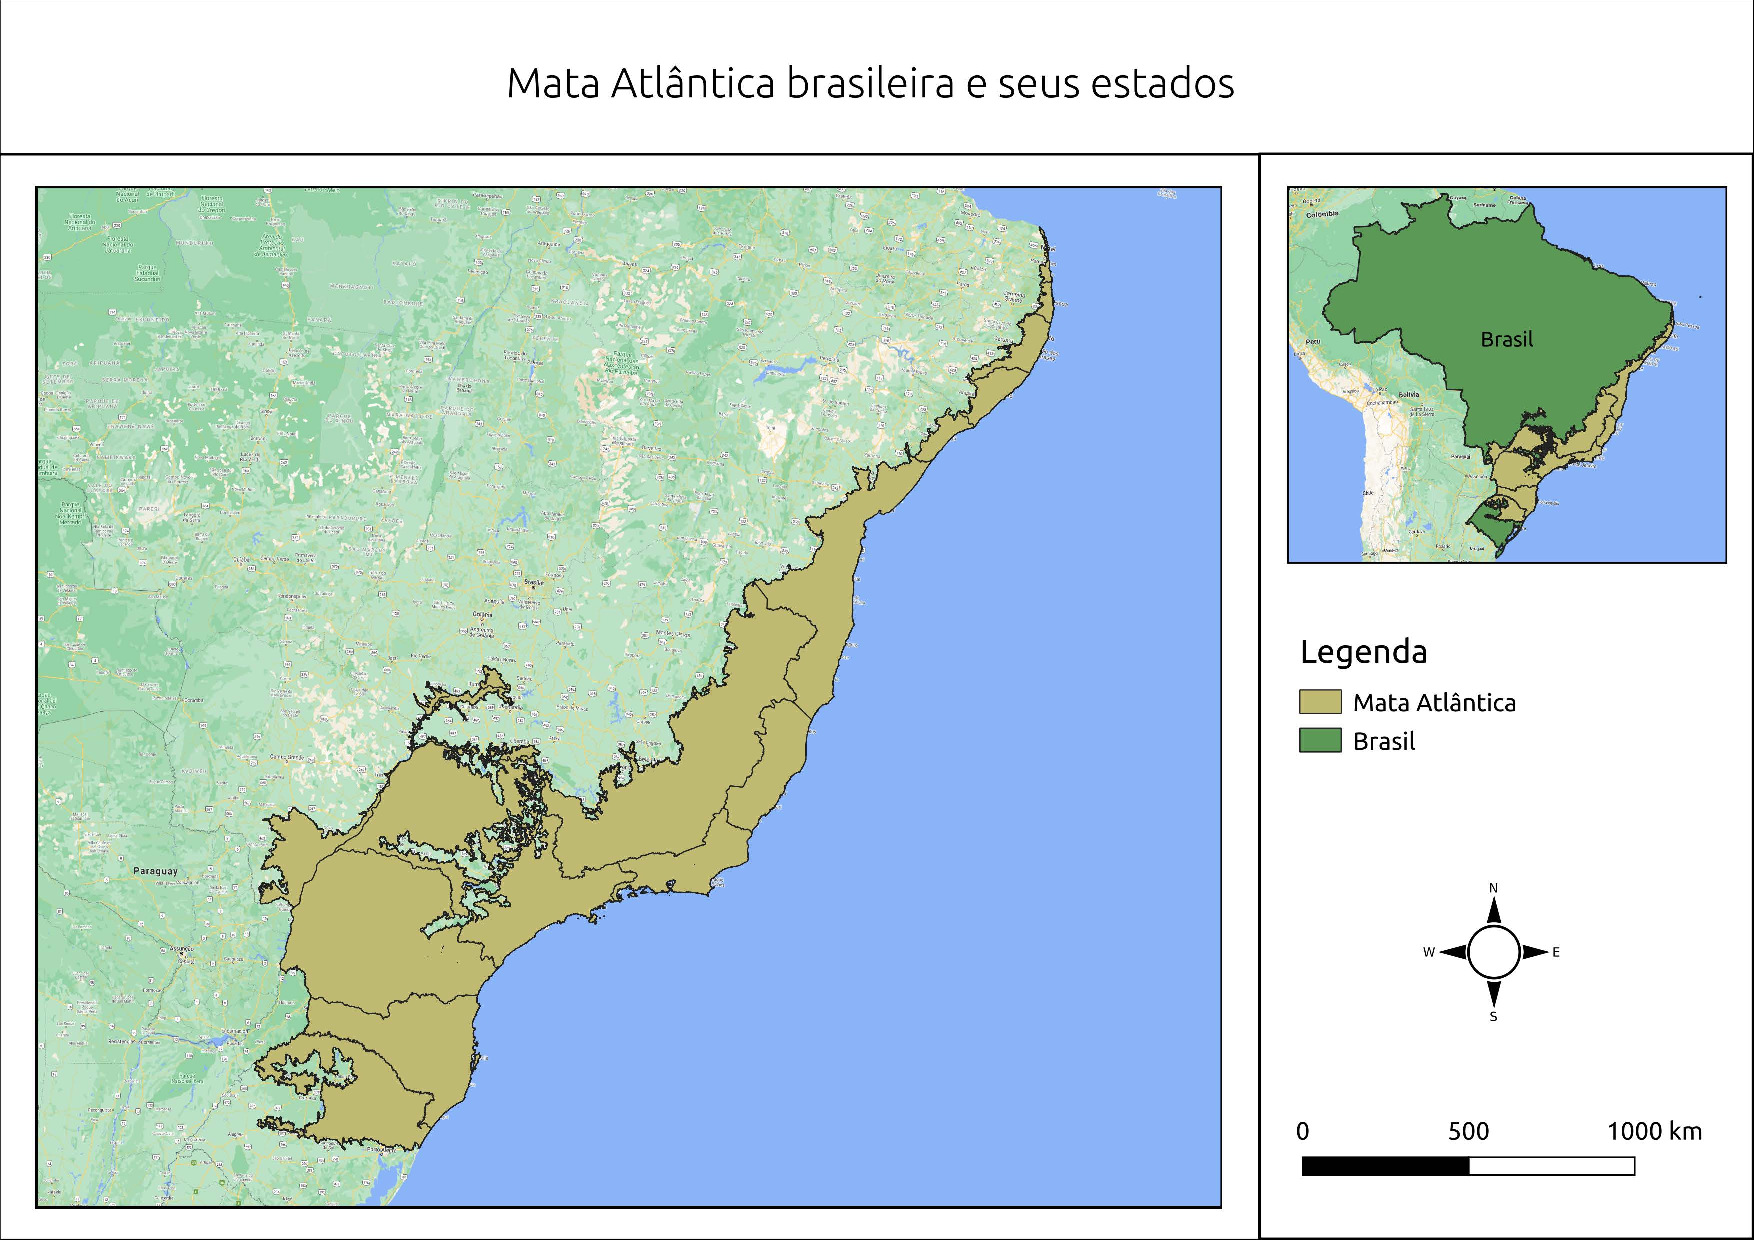
\includegraphics[scale=.5]{images/mata_atlantica.pdf}
    \caption{Área de Estudo - Mata Atlântica brasileira}
    \label{fig:mata_atlantica}
\end{figure}

Na época da chegada dos portugueses no Brasil, a Mata Atlântica cobria cerca de 1,5 milhões de quilômetros quadrados (incluindo ecótonos), estendendo-se ao longo de 3 mil quilômetros da costa brasileira - do Rio Grande do Sul ao Rio Grande do Norte - e penetrando pelo interior, cruzando São Paulo, Minas Gerais e Mato Grosso do Sul até as fronteiras da Argentina e do Paraguai \citep{scarano2014}. Cerca de 500 anos depois, esse extenso e representativo bioma abriga mais de 100 milhões de pessoas, cerca de 1/4 das quais ainda vivem na pobreza \citep{scarano2014}.

Segundo o projeto Mapbiomas \citep{Souza2019}, a área total de florestas no bioma em 1985 era de mais de 30 Mha e em 2018 de 28 Mha. Já a área de florestas que não sofreram mudanças significativas (pseudo-invariantes) durante o período de 1985 até 2018 foi de aproximadamente 21.4 Mha. Deste total, somente  30\% da vegetação nativa remanescente está protegida legalmente através de unidades de conservação.

% Apesar dos importantes avanços obtidos nesta agenda na última década – como a restauração de aproximadamente 1,4 milhões de hectares entre 2011 e 2020 – muito ainda precisa ser feito \citep{CROUZEILLES2019}

\subsubsection{Dados de entrada}
\hspace{13pt} Para o mapeamento do bioma consideramos um intervalo anual que compreendeu todos os anos de 1985 até 2018 utilizando imagens do satélite Landsat das séries 5, 7 e 8. A escolha desse período de análise se deu por conta do início da captura de dados em 1 de março de 1984 pelo satélite Landsat 5 e consequente disponibilidade de dados pela comunidade científica para o mesmo período, o que facilitou a verificação e validação dos resultados. Para cobrir todos os 110 Mha do bioma foi necessário a compilação e processamento de 88 cenas Landsat, cada cena cobrindo os 33 anos da análise com cerca de 23 imagens por ano, o que dá algo em torno de aproximadamente 67 mil imagens, o que representa quase 2.5x toda a quantidade de imagens Landsat utilizada em estudos no continente sul americano nos últimos 50 anos \citep{Hemati2021}. Se considerarmos que cada uma dessas imagens utilizadas possui pelo menos 7 bandas, chegamos a um cubo multidimensional de quase meio milhão de bandas. Um processamento que sem dúvidas só seria possível com o advento das tecnologias já citadas.

Todas as imagens utilizadas são da coleção \emph{surface reflectance}, o que significa que já possuem correção geométrica, radiométrica e possuem valor físico referente a superfície terrestre. Além disso, as imagens passaram por processo de harmonização para evitar acúmulo de ruídos e também de remoção de nuvens e sombras. Todos os processamentos para a composição das séries temporais foram feitos utilizando funções internas do próprio Landtrendr, o que facilitou em muito toda a etapa de preparação dos dados.

\subsubsection{Método de análise}
\hspace{13pt} A análise das trajetórias foi feita utilizando o algoritmo Landtrendr em sua versão para a plataforma Google Earth Engine (GEE) \citep{Kennedy2018}. A principal vantagem da implementação do algoritmo no GEE em relação a sua versão original em ENVI/IDL está na possibilidade de sua aplicação em áreas extensas com um tempo de pré-processamento e análise em si muito menores, o que possibilita sua aplicação em contextos anteriormente inviáveis. O ganho de tempo não está somente no tempo de processamento do algoritmo em si, como também na eliminação de grande parte dos desafios técnicos relacionados ao processamento dos dados de entrada presentes em sua implementação clássica. No entanto, apesar do ganho significativo no tempo de processamento, o Landtrendr para o GEE também apresenta algumas limitações quando comparado a sua versão em original em IDL. Uma das maiores está na limitação na extensão da análise para apenas uma imagem Landsat por vez. A plataforma apresentou erros sistemáticos quando requisitada para processar análises para toda a Mata Atlântica de uma só vez, ou para áreas que abrangiam vários estados, por exemplo. Com isso, o processamento teve de ser feito em etapas. 

As etapas tiveram de ser divididas por cenas Landsat, neste caso, 88 cenas (Figura \ref{fig:pathrow_centroids}). Como o resultado do algoritmo é dado de forma separada por cena, foi necessário juntar todas as camadas geradas. Devido a ruídos presentes nas bordas das imagens Landsat e a sobreposição natural entre imagens diferentes, nem todos os pixels presentes nas bordas apresentaram resultados similares. Juntar todos as 88 camadas de resultados em uma se tornou um desafio e só foi possível através da criação de polígonos de voronoi \citep{Okabe}, o que possibilitou utilizarmos somente as áreas mais próximas do centro das camadas geradas pelo algoritmo (Figura \ref{fig:voronoi_example}).

\begin{figure}[H]
    \centering
    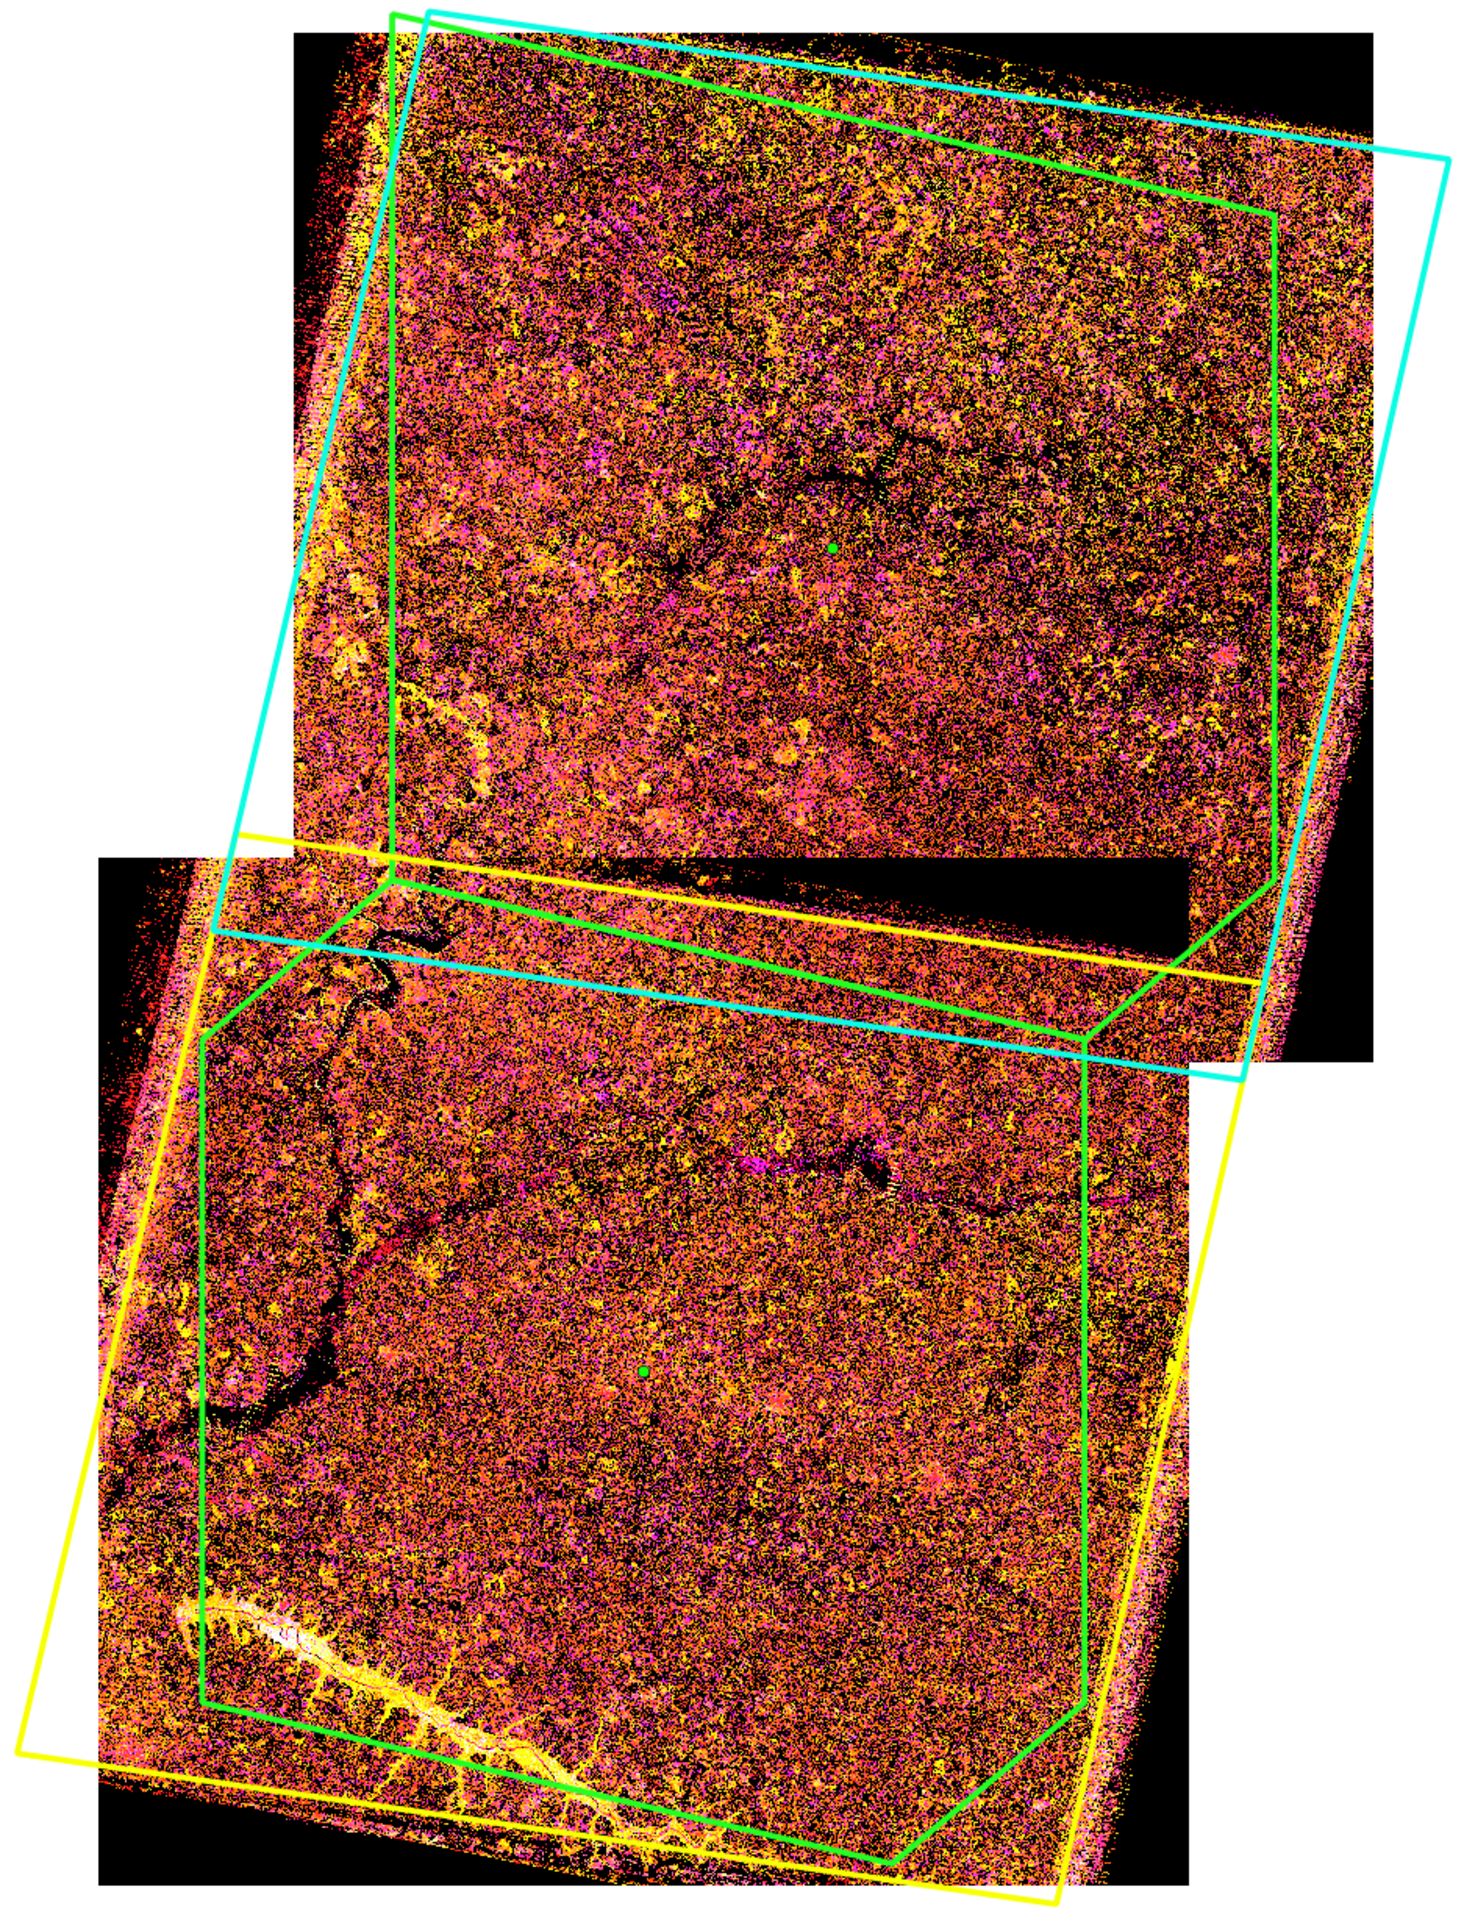
\includegraphics[scale=.5]{images/voronoi_example.pdf}
    \caption{No centro das duas imagens podemos ver os centroides em verde, assim como os polígonos de voronoi na mesma cor. Já em ciano e amarelo, podemos observar os polígonos envolventes para as cenas Landsat 222/73 e 222/74. As imagens de fundo são compostas pela composição das seis bandas geradas pelo Landtrendr para as duas cenas. É possível ver a presença de sobreposição entre os dois resultados a partir dos retângulos envolventes do satélite e também de sobreposição nos polígonos de voronoi.}
    \label{fig:voronoi_example}
\end{figure}

\begin{figure}[h!]
    \centering
    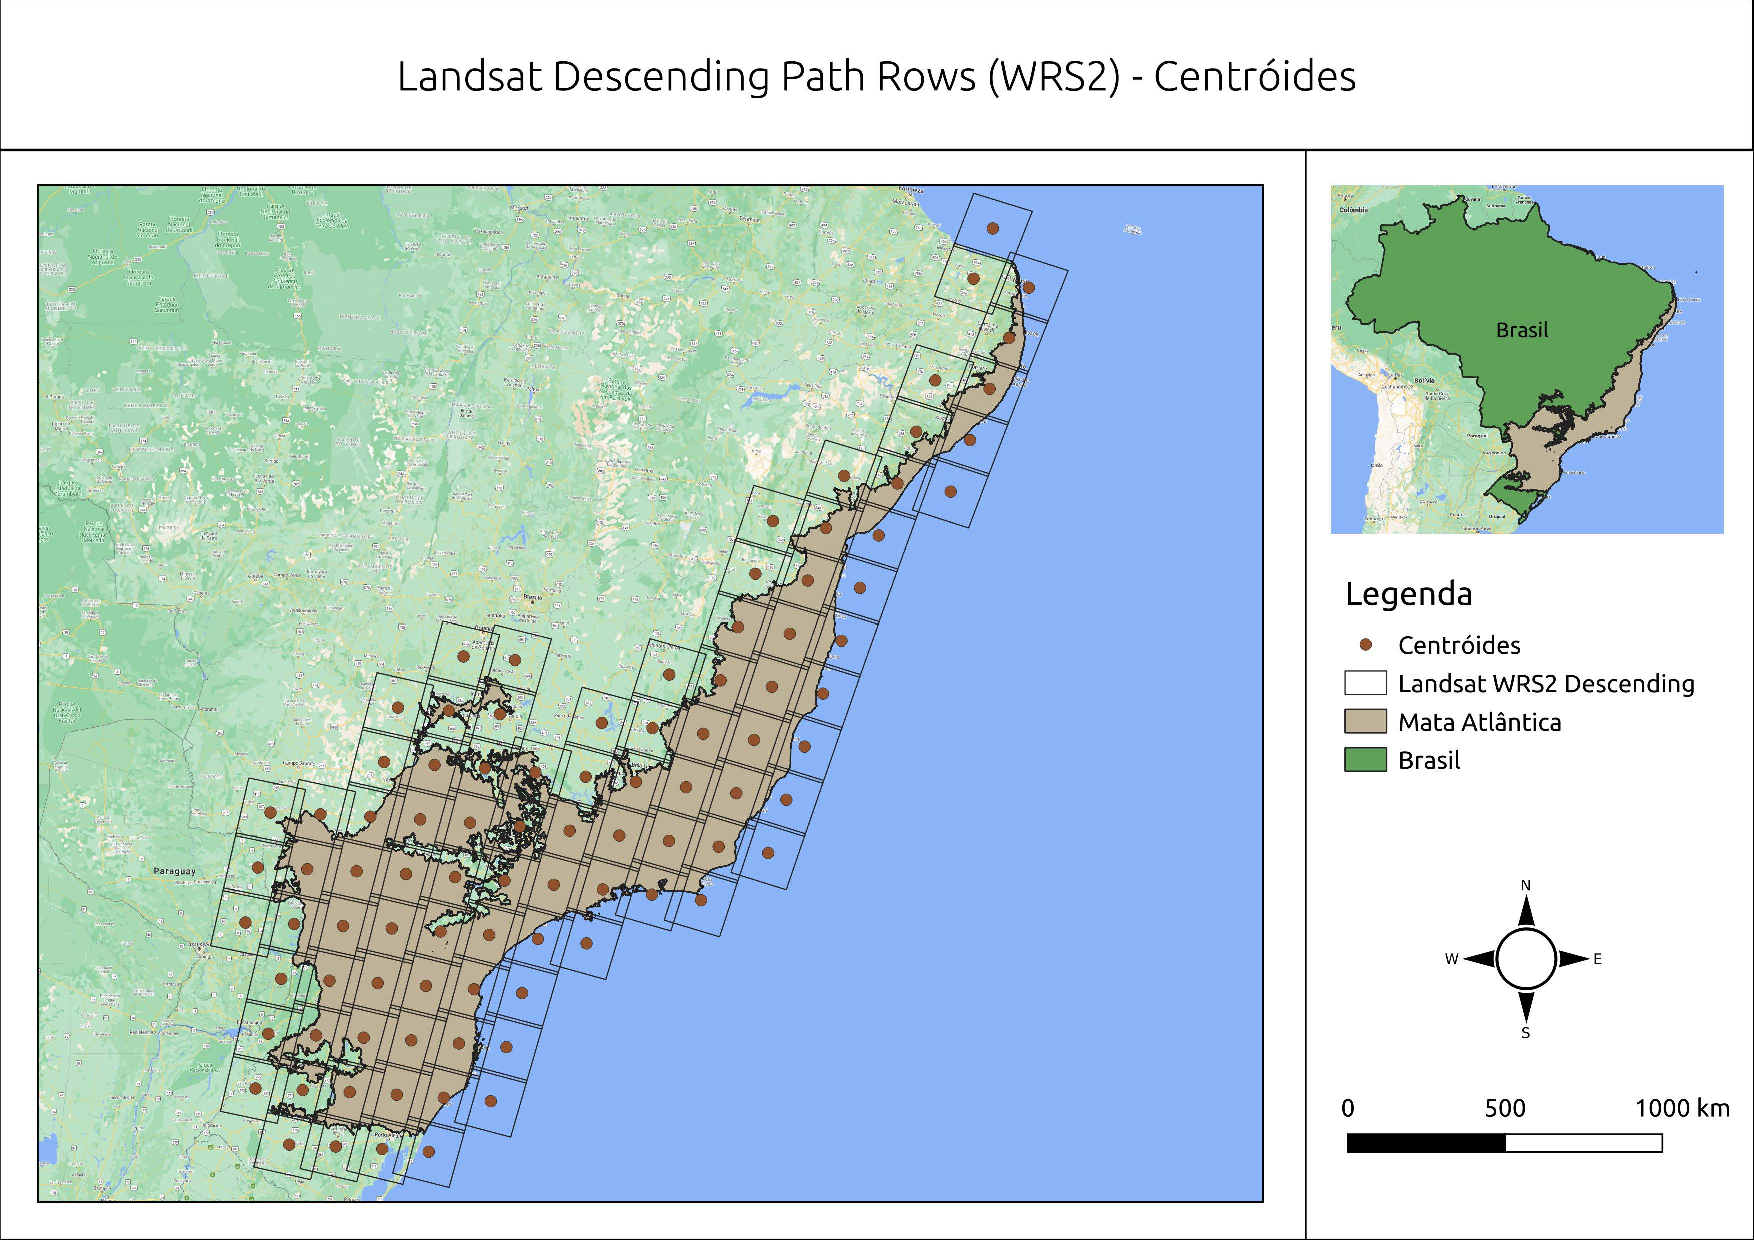
\includegraphics[scale=.5]{images/ma_pathrow_centroids.pdf}
    \caption{Pathrows das imagens Landasat e seus respectivos centróides que foram utilizados para delimitar as cenas a serem processadas pelo algoritmo}
    \label{fig:pathrow_centroids}
\end{figure}

Os polígonos de voronoi foram gerados através da extração dos centroides dos polígonos delimitadores das cenas Landsat e posteriormente utilizados para a criação dos polígonos com as áreas centrais (Figura \ref{fig:voronoi_ma}). Após a geração dos polígonos de voronoi, os mesmos foram utilizados para recortar os resultados de forma a limpar possíveis sobreposições. Após o recorte, todas as imagens foram agregadas para toda extensão do bioma e separadas banda a banda para análise posterior.

\begin{figure}[H]
    \centering
    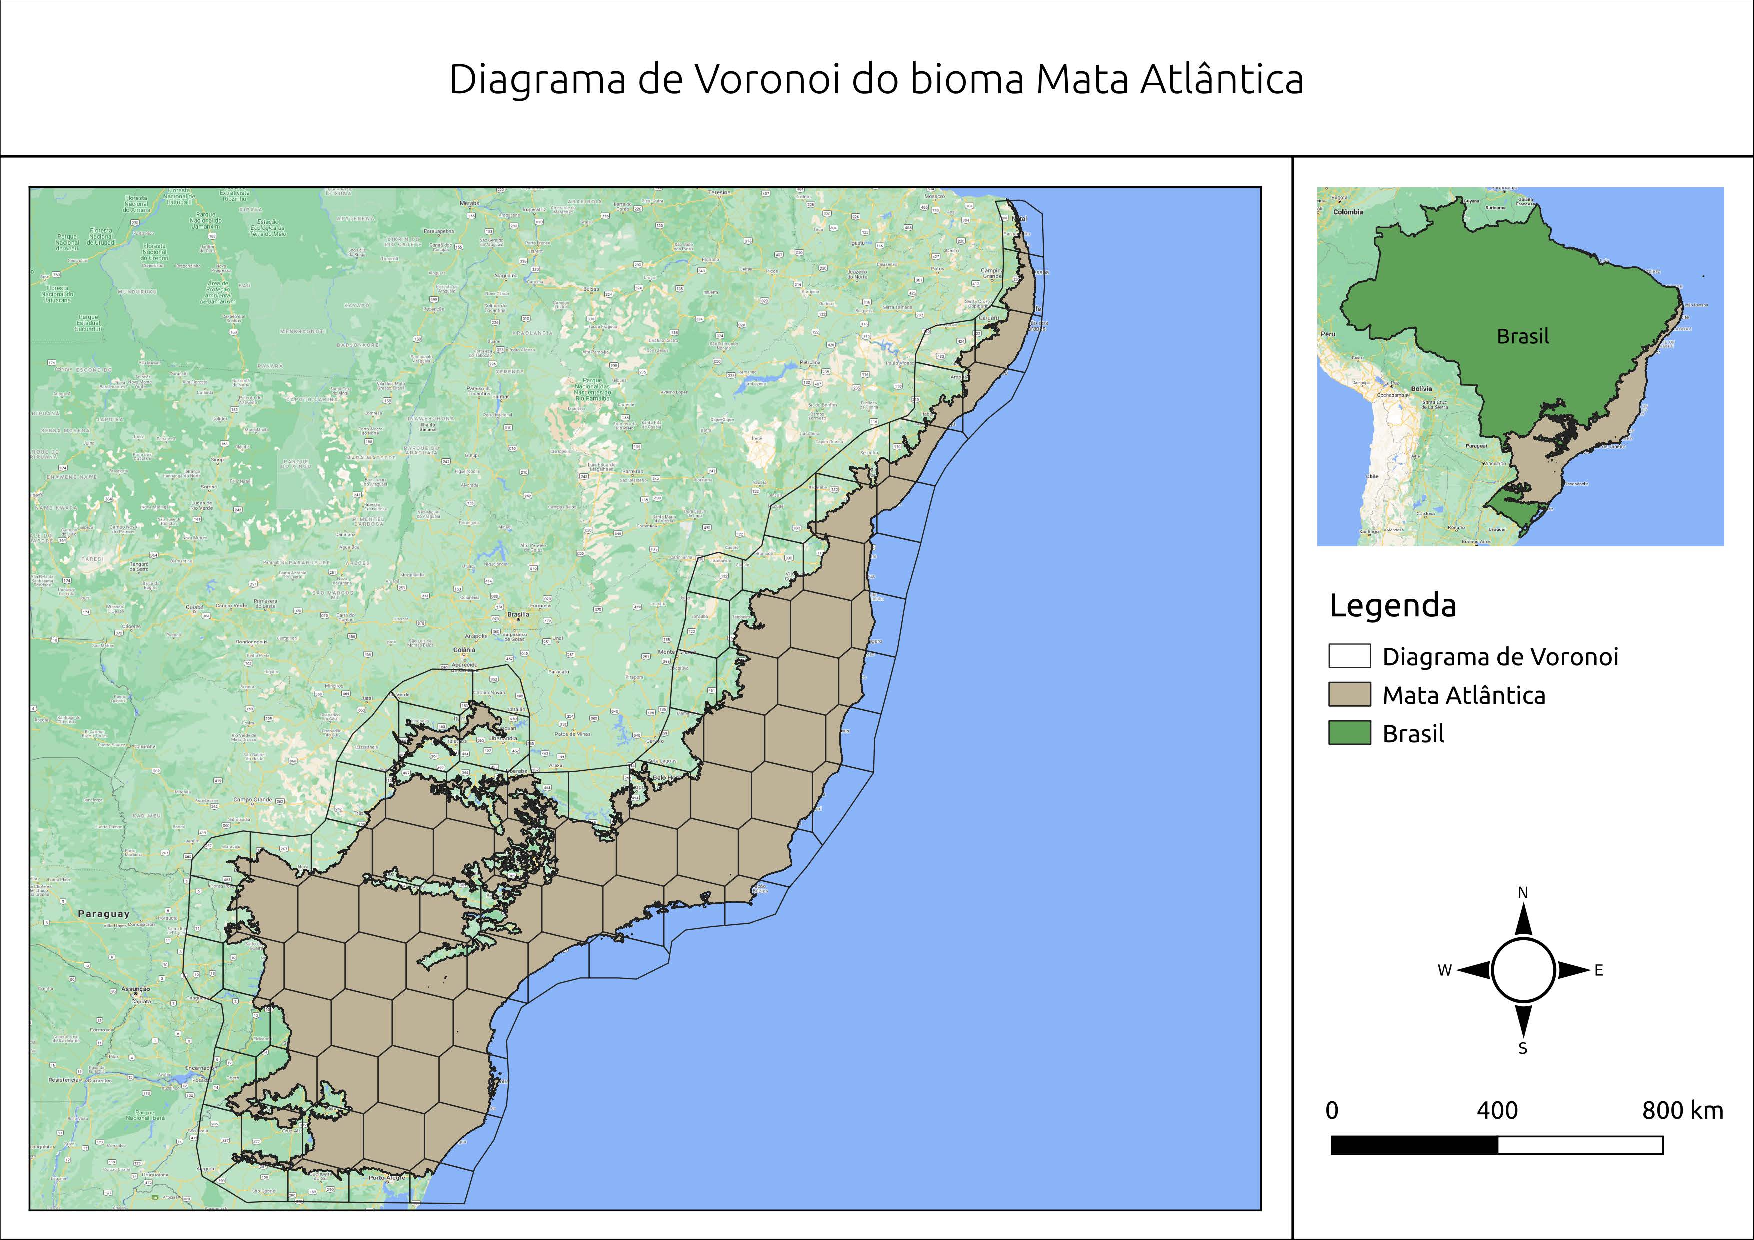
\includegraphics[scale=.5]{images/voronoi_mata_atlantica.pdf}
    \caption{Diagrama de Voronoi criado a partir dos centróides.}
    \label{fig:voronoi_ma}
\end{figure}

O algoritmo Landtrendr trabalha analisando os valores pixel a pixel para toda a composição de imagens visando criar segmentos e assim identificar trajetórias (Figura \ref{fig:landtrendr_graph}). O algoritmo pode gerar métricas tanto para distúrbios de perda como de ganho, além de detectar mudanças que ocorreram de forma lenta ou rápida, possibilitando também o cálculo da duração de eventos segmentados previamente gerando dados contínuos, discretos, assim como a duração e o ano da detecção. Podemos analisar, portanto, a história do pixel em questão, neste caso, sob uma perspectiva meso-escalar das florestas de Mata Atlântica. Para realizar o processo de segmentação temporal o algoritmo pode utilizar tanto uma banda padrão do satélite como algum índice espectral. Alguns índices já bem estabelecidos já estão implementados na ferramenta como o NDVI (\textit{Normalized Difference Vegetation Index}), o EVI (\textit{Enhanced vegetation index}), o NDMI (\textit{Normalized Difference Moisture Index}) e o NBR (\textit{Normalized Burn Ratio}). É possível também utilizar uma das próprias bandas do satélite para realizar as análises, como a banda do vermelho ou o SWIR (\textit{Short-wave infrared}). 

% Apesar de bandas como o NBR e NDMI mostrarem bons resultados em regiões de floresta temperada, testes realizados em florestas tropicais mostraram que índices como o NDVI apresentam resultados superiores \citep{zebende2019}. 
% Sendo assim, para este estudo, o processo de segmentação temporal foi realizado utilizando o NDVI como banda base.
% Adicionar todo o conteúdo sobre o CSNR (Change Signal to Noise Ratio).

\begin{figure}[h!]
    \centering
    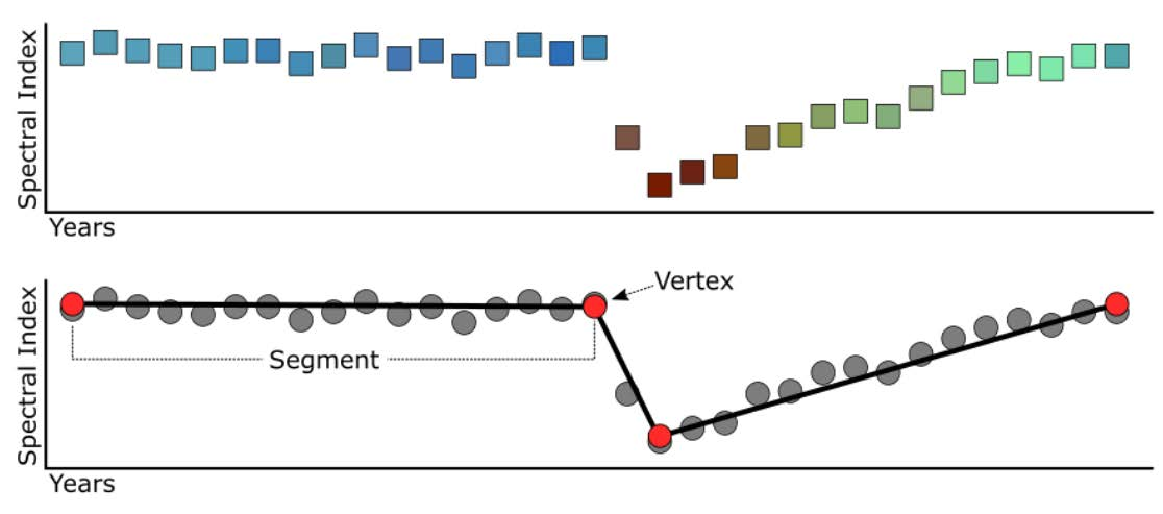
\includegraphics[scale=.8]{images/landtrendr_graphic.pdf}
    \caption{Segmentação temporal do pixel pelo algoritmo Landtrendr. \\ Fonte: Documentação oficial}
    \label{fig:landtrendr_graph}
\end{figure}

\subsubsection{Escolha da banda ou índice a ser analisado}

A escolha do índice a ser utilizado é parte importante do processo já que essa escolha pode influenciar na precisão do processo de identificação das mudanças de acordo com o que se está tentando detectar. O índice NBR, tradicional no monitoramento de queimadas vem mostrando excelentes resultados na detecção de mudanças em áreas de florestas temperadas, com resultados superiores a índices mais tradicionais como o próprio NDVI ou o EVI.

Em áreas tropicais, o uso de índices com o NDVI ainda é predominante \citep{zebende2019, FRAGAL2016}, mas devido a variabilidade na qualidade dos resultados de acordo com a banda ou índice utilizado, o algoritmo fornece como uma das camadas resultantes de cada análise realizada uma banda extra chamada CSNR (\textit{Change Signal to Noise Ratio}), que oferece uma métrica para entender qual banda pode ser ideal para cada tipo de região estudada. Como a mesma só pode ser gerada após a execução do algoritmo, é recomendado que o algoritmo seja primeiro executado para uma mesma área teste diversas vezes utilizando bandas e índices diferentes para cada rodada. Bandas/índices que obtiverem maior valor médio geral na camada CSNR possuem menor quantidade de erro associada ao processo de detecção de mudanças.

Sendo assim, o teste com a banda CSNR foi realizado para as 13 bandas/índices (Azul, Verde, Vermelho, NIR, SWIR, Tasseled Cap Brightness/Greenness/Wetness, NBR, NBRz, NDVI, EVI e NDMI) presentes no algoritmo para cada uma das fitofisionomias estudadas no bioma neste estudo (Tabela \ref{tab:csnr_results}). 


\begin{table}[h!]
    \centering
    \rowcolors{2}{red!50!yellow!30}{green!40!yellow!10}
    % \footnotesize
    \begin{tabular}{| c | c | c| c | c |}
    \hline
            Camada & Est. Semidecidual & Omb. Mista & Omb. Densa & Média \\
            SWIR & 2.53 & \textbf{3.47} & \textbf{3.00} & \textbf{3.00} \\
            Vermelho & 2.49 & 3.25 & 2.93 & 2.89 \\
            TCW & 2.40 & 3.26 & 2.95 & 2.87 \\
            Verde & 2.42 & 3.16 & 2.76 & 2.78 \\
            TCB & \textbf{2.58} & 3.05 & 2.66 & 2.77 \\
            EVI & 2.56 & 2.82 & 2.87 & 2.75 \\
            NDMI & 2.27 & 2.86 & 2.98 & 2.70 \\
            NDVI & 2.40 & 2.85 & 2.86 & 2.70 \\
            NBR & 2.27 & 2.90 & 2.81 & 2.66 \\
            NBRz & 2.25 & 2.88 & 2.81 & 2.65 \\
            TCG & 2.05 & 2.19 & 2.53 & 2.26 \\
            NIR & 2.06 & 2.17 & 2.31 & 2.18 \\
            Azul & 1.92 & 2.36 & 2.19 & 2.16 \\
    \hline
    \end{tabular}
    \caption{Mediana dos valores da camada CSNR para cada banda/índice em cada fitofisionomia (Estacional Semidecidual, Ombrófila Mista e Ombrófila Densa). A última coluna representa a média geral da banda/índice considerando todas as medianas obtidas em todas as fitofisionomias.}
    \label{tab:csnr_results}
\end{table}

Podemos observar que de forma geral os melhores resultados se concentraram nas regiões de floresta ombrófila com uma maior quantidade de ruído nas regiões estacionais, resultado de certa forma já esperado devido a maior interferência estrutural devido ao ciclo das estações. Mesmo analisando composições anuais, podemos perceber que existe interferência no valor mediano em regiões estacionais suficiente para influenciar na geração de ruídos. Apesar disso, o acréscimo de ruídos nas regiões estacionais não impactou o resultado final a ponto de influenciar a acurácia global de forma significativamente negativa.

Quanto aos índices disponíveis, nenhum apresentou resultado superior para todas as fitofisionomias. Para as áreas de vegetação ombrófila, a banda do SWIR apresentou o melhor resultado tanto nas áreas mistas quanto densas. Já nas áreas semideciduais, o melhor resultado se deu com os valores de bilho do Tasseled Cap, seguido do EVI. O tradicional NDVI obteve um resultado geral mediano, tecnicamente empatado com o NDMI. Já na média geral, foi o SWIR que obteve melhor resultado. O NBR, índice recorrente em trabalhos aplicados a áreas temperadas não se saiu tão bem em ambientes tropicais, mas se posicionando logo abaixo do NDVI.

Apesar desses resultados iniciais, um novo teste foi realizado. Desta vez, uma nova área de teste dentro de florestas ombrófilas densas foi adicionada com o intuito de entender se os resultados obtidos se manteriam similares entre fitofisionomias semelhantes. A área escolhida foi dentro da Bacia Hidrográfica do Rio Sâo João (BHRSJ). Através do novo teste, foi possível observar que houve grande variabilidade na escolha dos melhores índices/bandas mesmo em regiões similares. Desta vez, a banda do vermelho obteve o melhor resultado, seguido do NDVI, o que fez a média geral do índice normalizado subir (Tabela \ref{tab:csnr_results_com_bhrsj}).


\begin{table}[h!]
    \centering
    \rowcolors{2}{red!50!yellow!30}{green!40!yellow!10}
    % \footnotesize
    \begin{tabular}{| c | c | c | c| c | c |}
    \hline
            Camada & BHRSJ & Est. Semidecidual & Omb. Mista & Omb. Densa & Média \\
            SWIR & 3.09 & 2.53 & \textbf{3.47} & \textbf{3.00} & \textbf{3.02} \\
            Vermelho & \textbf{3.35} & 2.49 & 3.25 & 2.93 & 3.00 \\
            TCW & 3.00 & 2.40 & 3.26 & 2.95 & 2.90 \\
            Verde & 3.15 & 2.42 & 3.16 & 2.76 & 2.87 \\
            NDVI & 3.25 & 2.40 & 2.85 & 2.86 & 2.84 \\
            TCB & 2.86 & \textbf{2.58} & 3.05 & 2.66 & 2.79 \\
            NDMI & 3.00 & 2.27 & 2.86 & 2.98 & 2.78 \\
            EVI & 2.85 & 2.56 & 2.82 & 2.87 & 2.77 \\
            NBRz & 2.94 & 2.25 & 2.88 & 2.81 & 2.72 \\
            NBR & 2.88 & 2.27 & 2.90 & 2.81 & 2.71 \\
            TCG & 2.93 & 2.05 & 2.19 & 2.53 & 2.43 \\
            NIR & 2.68 & 2.06 & 2.17 & 2.31 & 2.31 \\
            Azul & 2.40 & 1.92 & 2.36 & 2.19 & 2.22 \\
    \hline
    \end{tabular}
    \caption{Mediana dos valores da camada CSNR para cada banda/índice em cada fitofisionomia (Estacional Semidecidual, Ombrófila Mista e Ombrófila Densa). A última coluna representa a média geral da banda/índice considerando todas as medianas obtidas em todas as fitofisionomias.}
    \label{tab:csnr_results_com_bhrsj}
\end{table}

Observando os resultado obtidos, entende-se que a escolha do índice ou banda a ser utilizada para a análise dependa muito mais do que se busca detectar do que necessariamente a camada com maior valor obtido pela banda CSNR. Além disso, para áreas de estudo extensas, é possível que não exista coerência entre os resultados para áreas em teoria similares. Essas diferenças acabam reforçando ainda mais a preocupação com o uso de bandas e índices já conhecidos e estudados anteriormente de acordo com cada contexto.

Entende-se também ser possível utilizar índices que obtiveram o melhor resultado para cada caso como o do SWIR no caso de florestas ombrófilas e do TCB para áreas de florestas estacionais semideciduais para estudos que envolvam áreas mais restritas. Outra possibilidade analisada através dos resultados obtidos é a utilização de uma combinação de bandas/índices diferentes para áreas extensas que envolvam uma ou mais fitofisionomias. No entanto, é necessário pensar no custo-benefício dessa escolha, já que a mesma envolveria uma série de testes e processos fragmentados, elevando significativamente o tempo total de execução e viabilidade do estudo. 

Neste trabalho, o NDVI foi utilizado para a detecção de mudanças para toda a extensão do bioma. Esta escolha se deu com o objetivo de testar o desempenho final do resultados buscando entender se a escolha de um único índice, principalmente um tradicional com o NDVI, pode gerar resultados satisfatórios para áreas extensas de floresta tropical. A utilização de uma única camada tem ainda como objetivo facilitar o processo de interpretação geral e de contribuir com análises comparativas entre fitofisionomias. A escolha do índice significa apenas uma etapa do processo, sendo necessário pensar a escolha de outros parâmetros.

Tanto os resultados para o cenário de perda quanto de ganho foram gerados com o objetivo de detectar supressões e processos de degradação, assim como de restauração e regeneração da floresta (Figura \ref{fig:flowchart_medologia_landtrendr}). Para este estudo, o Landtrendr foi aplicado utilizando todos seus parâmetros padrões. Os tipos de eventos (perda ou ganho) foram organizados de acordo com seu maior evento/segmento (\textit{Greatest Loss / Greatest Gain}).

Posterior aos resultados obtidos pelo algoritmo, toda a etapa de pós-processamento dos dados gerados no GEE foi desenvolvida em ambiente \textit{offline} utilizando ferramentas \textit{open source} como o QGIS \citep{QGIS_software}, GDAL \citep{gdal}, e a linguagem de programação R \citep{Rsoftware}, utilizando os pacotes Raster \citep{raster}, Terra \cite{terra}, gdalUtils \citep{gdalutils} e MLR \citep{mlr}.

\begin{figure}[H]
    \centering
    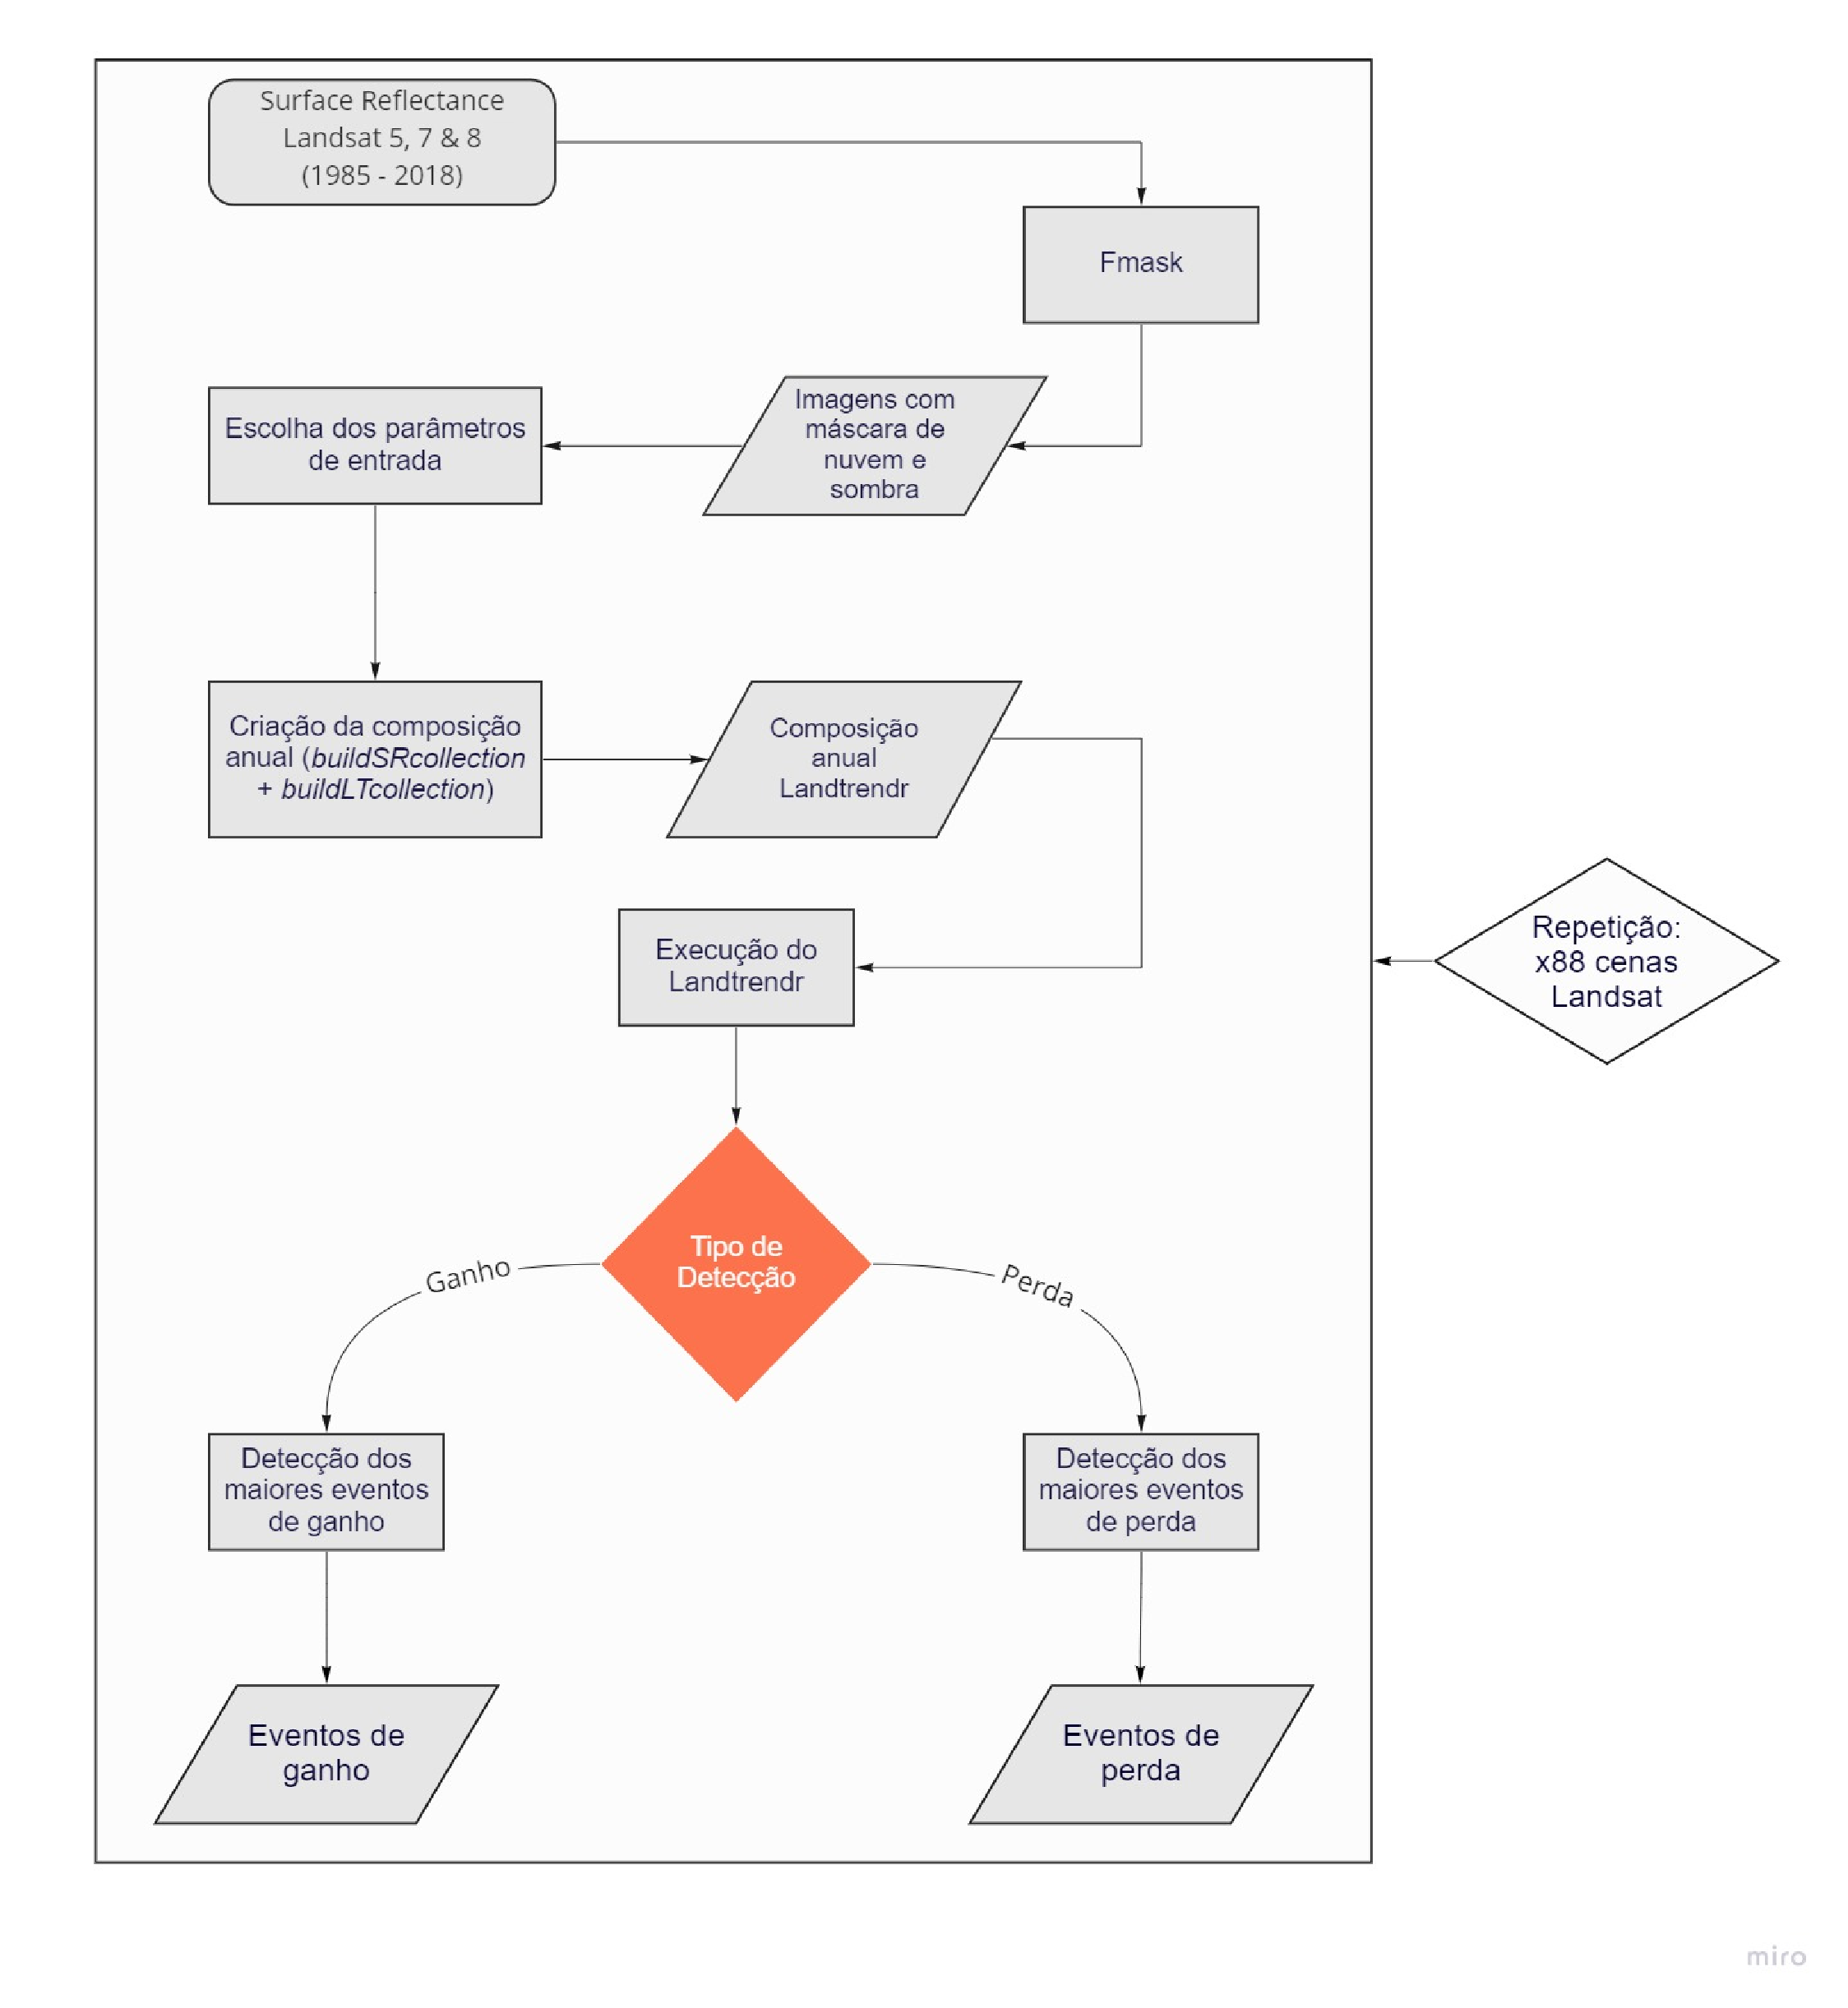
\includegraphics[scale=.5]{images/flowchart_medologia_landtrendr.pdf}
    \caption{Fluxograma do processo de execução do algoritmo Landtrendr}
    \label{fig:flowchart_medologia_landtrendr}
\end{figure}

\subsubsection{Processamento dos cenários de ganho}

\hspace{13pt} Para o cenário de ganho, todos os parâmetros padrão do algoritmo foram mantidos sem nenhum tipo de restrição. Ou seja, \textit{Max Segments} \textbf{6}, \textit{Spike Threshold} \textbf{0.9}, \textit{Vertex Count Overshoot} \textbf{3}, \textit{Prevent One Year Recovery} \textbf{true}, \textit{Recovery Threshold} \textbf{0.25}, \textit{p-value Threshold} \textbf{0.05}, \textit{Best Model Proportion} \textbf{0.75} e \textit{Min Observations Needed} \textbf{6}. Cenários de magnitude (\textit{magnitude}), valor prévio (\textit{previous value}), ano de detecção (\textit{year of detection}), duração (\textit{duration}) e taxa (\textit{rate}) foram gerados e posteriormente pós-processados para limpeza de ruídos e para retirada de valores indesejados. 

Primeiramente, foi gerado uma máscara com todas as áreas pseudo-invariantes entre os anos da análise (1985 - 2018) com o intuito de limpar detecções de mudança muito pequenas. Esta máscara representa todos os pixels que não tiveram nenhum tipo de mudança significativa durante todos os anos da análise, ou seja, áreas que em 1985 já eram consideradas floresta e que se mantiveram praticamente iguais até 2018 (Figura \ref{fig:flowchart_ganho}). 

Inicialmente esta máscara foi desenvolvida utilizando composições anuais de imagens Landsat considerando todos os anos da análise e posteriormente classificadas com o algoritmo Random Forest implementado no pacote MLR \citep{mlr}. No entanto, apesar de apresentar resultados promissores quando a aplicada no mapeamento da área teste na Bacia Hidrográfica do Rio São João, acabou demonstrando problemas quando extrapolada para o resto do bioma e se mostrou uma técnica altamente custosa tanto no tempo de processamento como no tempo de preparação dos dados de entrada \citep{LACERDA2021}. Apesar de não ter sido utilizada como uma máscara neste estudo, a técnica de identificação de áreas pseudo-invariantes utilizando técnicas de aprendizado de máquina pode ser de extrema valia quando aplicada em áreas menores.

Sendo assim, uma abordagem alternativa foi adotada para a criação da máscara para todo o bioma. Camadas de resultado do projeto Mapbiomas v4 foram utilizadas como uma \textit{proxy}. Todas as imagens classificadas para o bioma foram reclassificadas ano a ano em formato binário (floresta [1] e não-floresta [0]) e posteriormente multiplicadas entre si. Um \textit{raster} final binário foi então gerado, onde os pixels com valor 1 representavam áreas que permaneceram como floresta durante todos os anos do estudo e os de valor 0 todos os outros cenários, incluindo além de áreas que presenciaram algum tipo de mudança maior, todas as outras classes mapeadas pelo projeto. Somente pixels da classe floresta (classe número 3) da série 4 foram utilizados. Pixels de classes como floresta plantada foram excluídos assim como o todas as outras. Esta máscara evitou que muitos eventos pudessem ser classificados como ganho, apesar de terem baixa magnitude, já que representavam apenas um processo natural nas florestas já existentes. É importante notar que não estamos nos referindo a áreas de regeneração natural, mas de áreas pseudo-invariantes com variações mínimas durante o período do estudo. 

Além disso, foram mascarados todos os eventos com duração menor ou igual a 4 anos, já que não gostaríamos de incorporar eventos ainda muito recentes ou curtos que poderiam ser identificados como falsos eventos de mudança. O valor mínimo de 5 anos para eventos de ganho ajudou a identificar apenas eventos mais longos que tiveram tempo de apresentar respostas espectrais significativas de recuperação. Com 5 anos a vegetação já passa a apresentar um estágio sucessional característico de floresta secundária inicial \citep{Chazdon2014}. 

\begin{figure}[H]
    \centering
    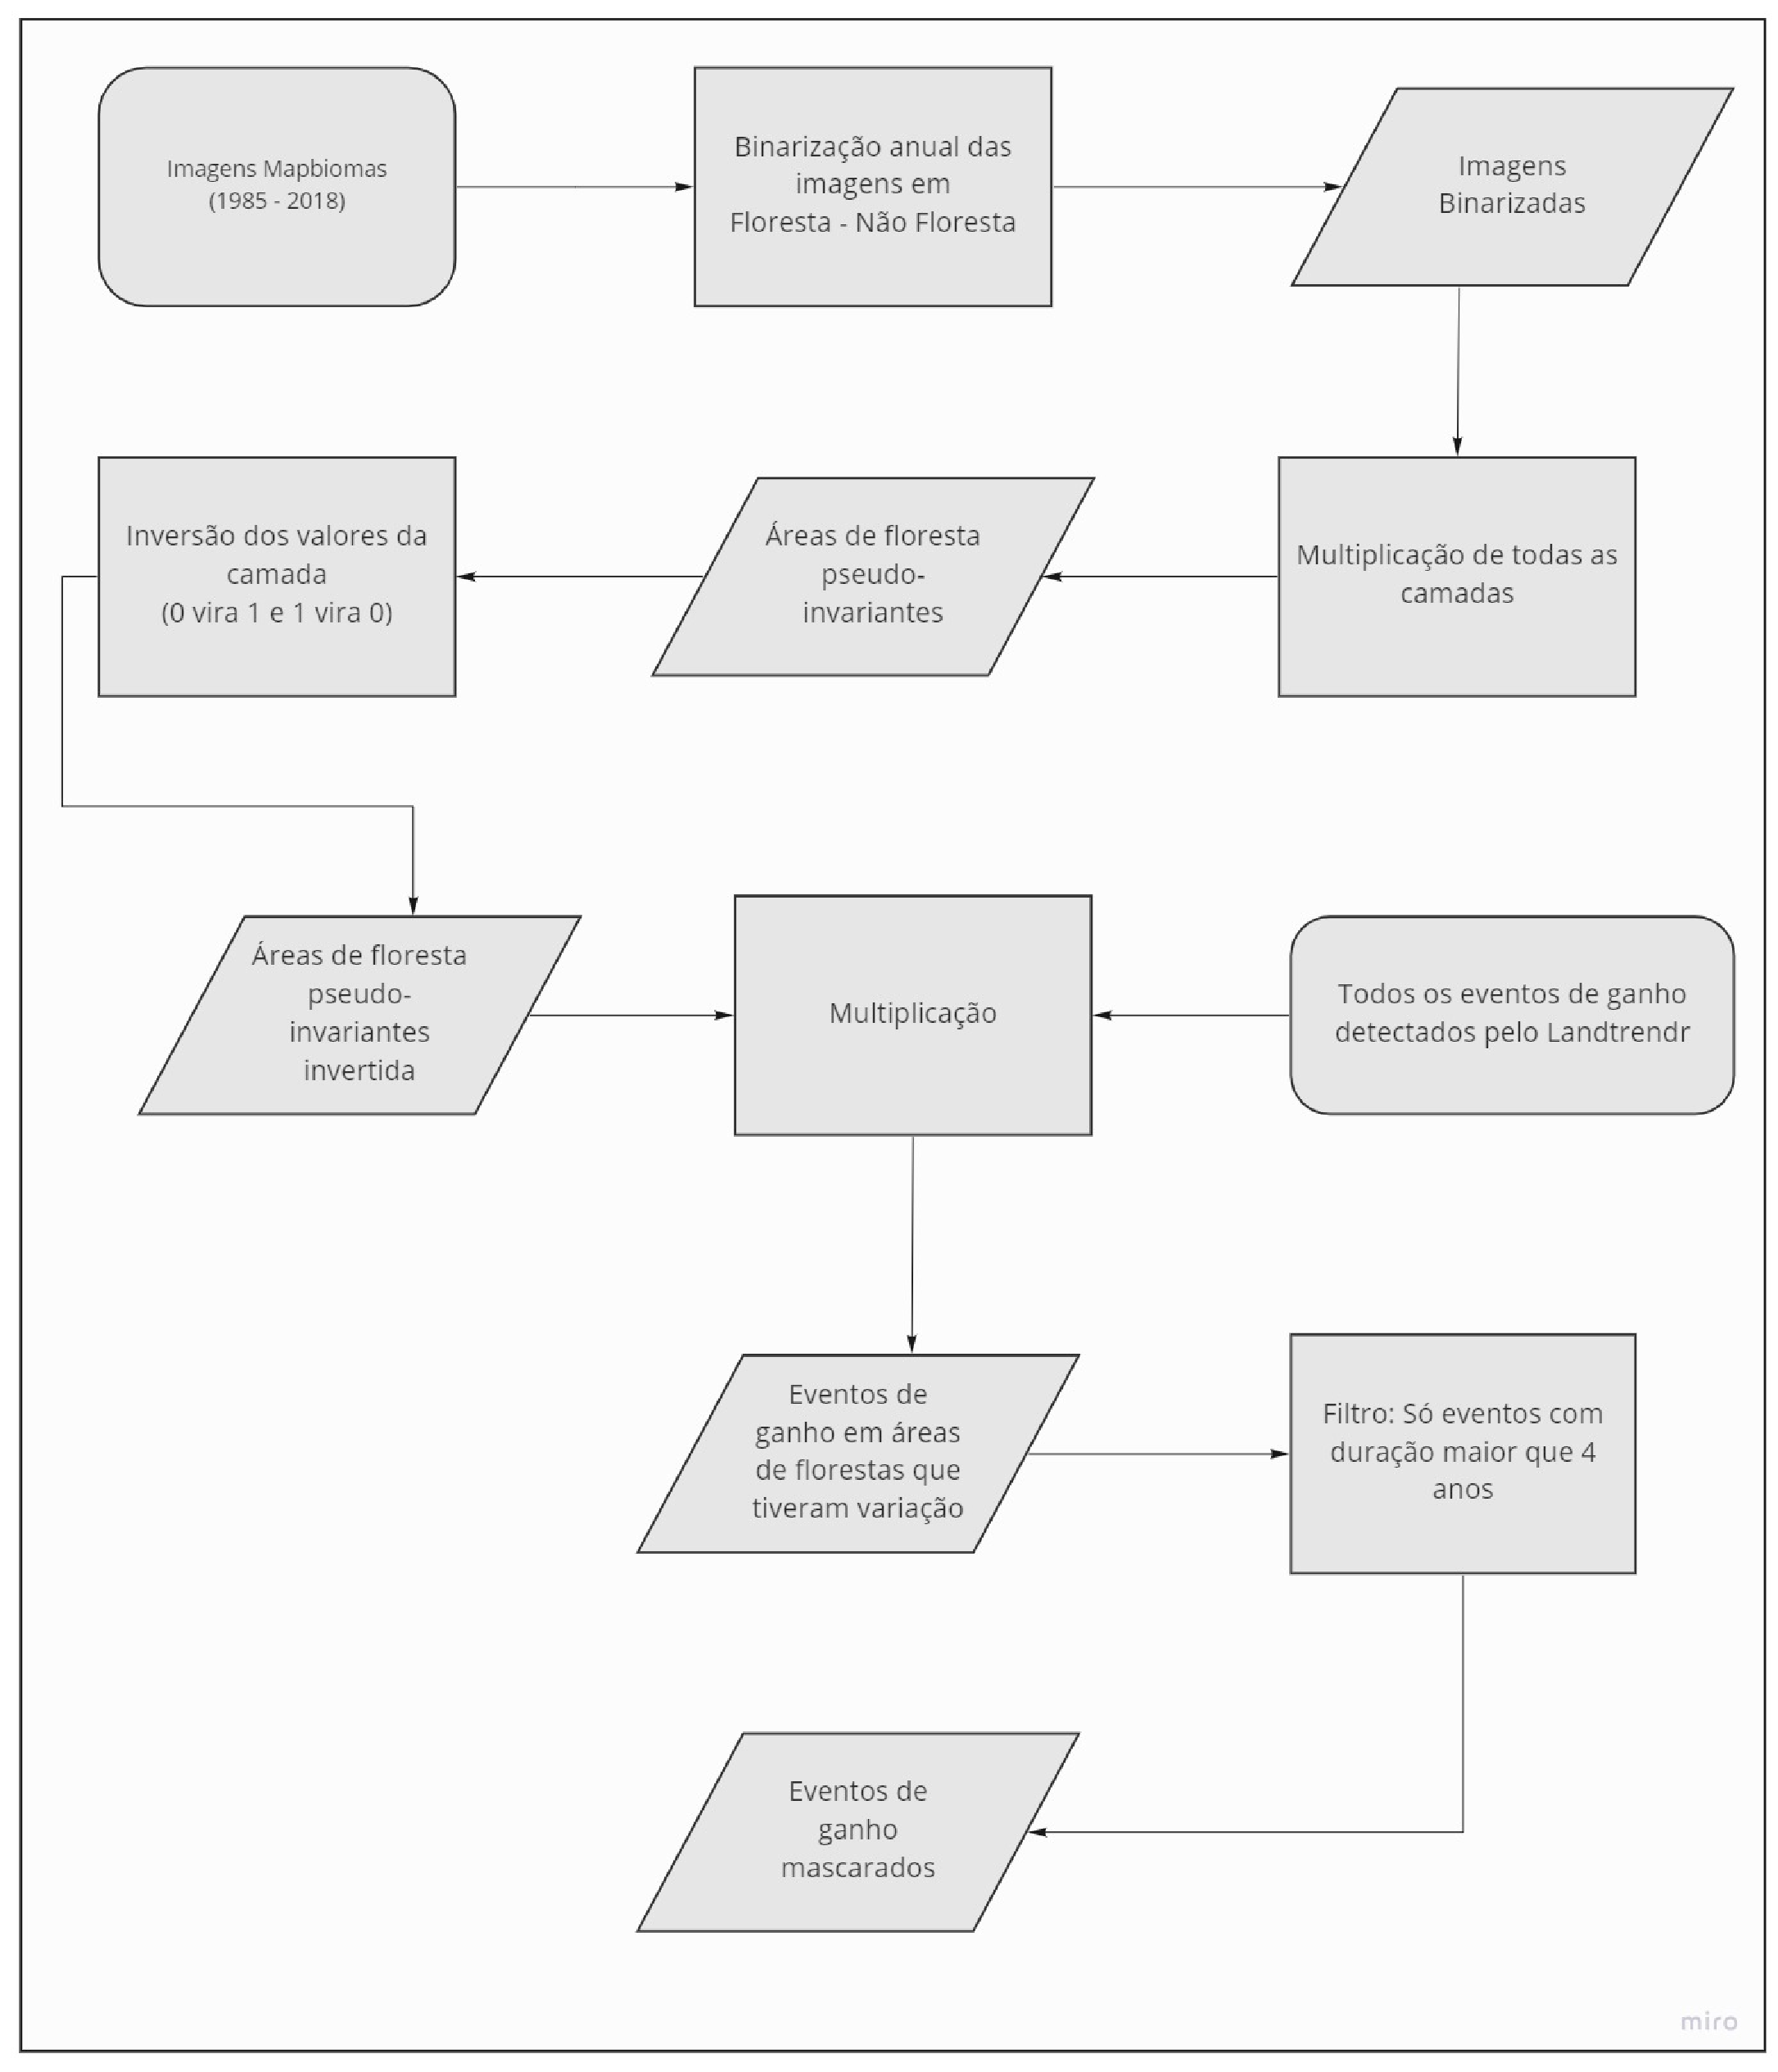
\includegraphics[scale=.4]{images/flow_ganho.pdf}
    \caption{Fluxograma do processo de pós processamento dos dados de ganho}
    \label{fig:flowchart_ganho}
\end{figure}

% figura para ilustrar?

\subsubsection{Processamento dos cenários de perda}
\hspace{13pt} Assim como o cenário de ganho, o processamento do cenário de perda utilizou todos os parâmetros padrões do algoritmo sem nenhum tipo de restrição com o objetivo de realizar limpezas nos resultados obtidos apenas na etapa de pós-processamento. Os mesmos cenários de magnitude (\textit{magnitude}), valor prévio (\textit{previous value}), ano de detecção (\textit{year of detection}), duração (\textit{duration}) e taxa (\textit{rate}) também foram gerados.

No caso das perdas, diferente do cenário de ganho, criou-se uma máscara para garantir que o Landtrendr fosse capaz de detectar mudanças de perda apenas em áreas que foram classificadas como floresta pelo projeto Mapbiomas no ano de 1985. Essa máscara ajudou na não seleção de áreas que nem mesmo tinham sido classificadas como florestas mas que sofreram algum tipo de perda com magnitude grande o suficiente para ser detectada pelo algoritmo. Além disso, uma outra máscara foi gerada para excluir áreas que apesar de terem sido mapeadas em 1985 como floresta e terem sofrido algum tipo de perda significativa, sofreram algum processo de restauração ou regeneração natural ao longo dos anos. Sendo assim, o resultado final para o dado de perdas visou somente a seleção de áreas que tiveram floresta, mas que perderam essa vegetação e não apresentaram nenhum processo de recuperação significativa posterior (Figura \ref{fig:flowchart_perda}).

Diferentemente dos dados de ganho, os dados de perda tem como característica importante a grande variabilidade na duração dos eventos. Sendo assim, utilizou-se a camada de duração para gerar, além das camadas de perda gerais, camadas de perda com duração igual a um ano e camadas com duração superior à um ano. Esta diferenciação é importante para que possamos identificar eventos de perda rápida, sejam eles de natureza antrópica ou natural, normalmente associados à cortes rasos ou queimadas.

\begin{figure}[H]
    \centering
    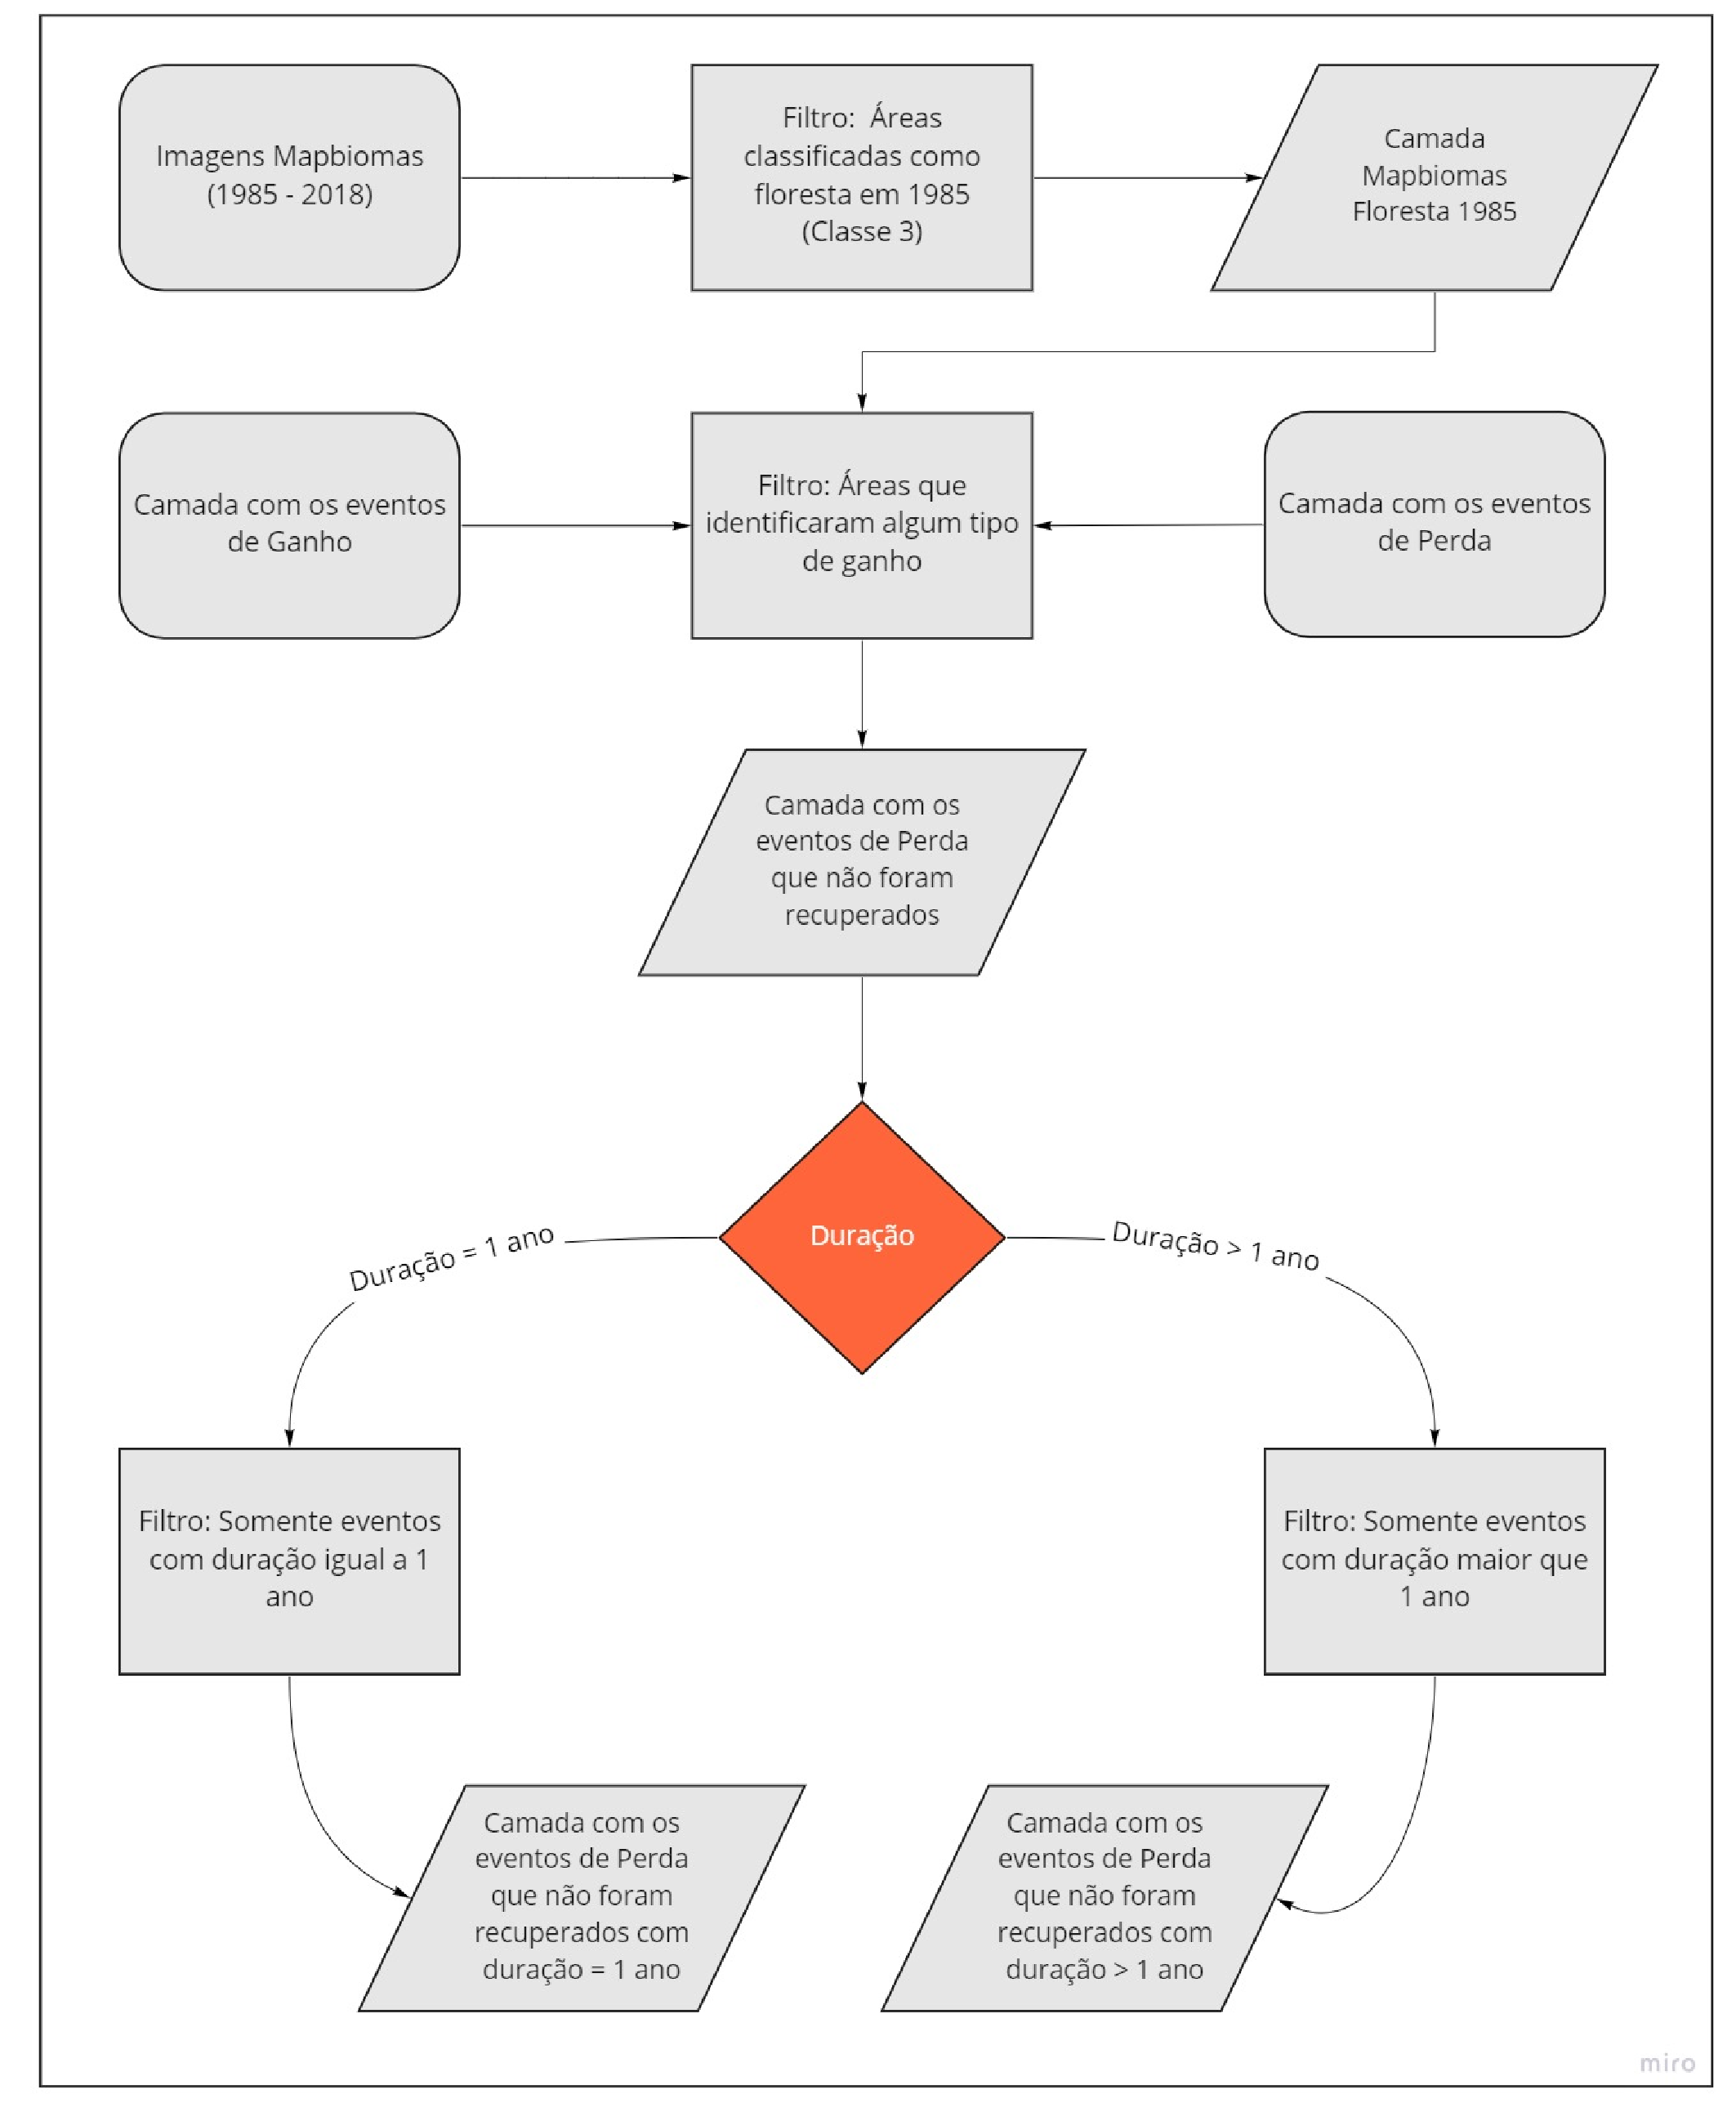
\includegraphics[scale=.4]{images/flow_perda.pdf}
    \caption{Fluxograma do processo de pós processamento dos dados de perda}
    \label{fig:flowchart_perda}
\end{figure}

\subsubsection{Escolha dos limiares para a filtragem dos eventos de mudança}
\hspace{13pt} Para além da filtragem das áreas de interesse, é interessante que, em alguns casos, uma segunda etapa de filtragem seja realizada para garantir que mesmo nas áreas de interesse, os pixels detectados como eventos de mudança pelo algoritmo estejam realmente dentro do esperado e façam sentido dentro do contexto da análise. 

Para isso, o Landtrendr possui a possibilidade de especificação de parâmetros de filtragem (\textit{Change Mapping Parameters}). Através da especificação desses parâmetros é possível realizar, já na execução do algoritmo, a filtragem dos eventos de acordo com a magnitude, duração e valor prévio (\textit{Pre-Dist Value}) do evento. 

É possível, por exemplo, a filtragem de todos os maiores eventos de perda que possuam duração maior que 4 anos, com magnitude maior que 400 e valor prévio maior que 600. No entanto, ao aplicar o algoritmo no contexto da Mata Atlântica, foi possível observar que a variabilidade de contextos espaciais pode implicar em muitos casos na filtragem de eventos indesejáveis, ou seja, falso-negativos. Apesar da facilidade apresentada pela implementação do algoritmo, fica evidente a necessidade da condução de testes para o maior entendimento da região a ser mapeada antes da aplicação de qualquer filtro deste tipo. A possibilidade de uso de filtros prévios acabam beneficiando apenas situações onde a área a ser mapeada foi previamente estudada ou em situações onde o resultado deve se restringir apenas a algumas características específicas.

Para este estudo, um filtro especificando um limiar para os eventos de perda era necessário. Muitos eventos com pouca magnitude foram detectados, representando áreas que houveram perdas, mas não significativas o suficiente ao longo da série para representar uma real mudança no uso e cobertura do solo.   

Sendo assim, testes foram realizados tanto para áreas de florestas ombrófilas densas quanto estacionárias semideciduais, já que era possível que o valor do limiar pudesse ser diferente de acordo com a fitofisionomia estudada. Cem amostras foram coletadas para cada fitofisionomia de floresta como também para áreas de pasto dentro de cada contexto. O valor médio de NDVI encontrado para áreas de floresta estacionária foi de 0.80 e ombrófila de 0.86. Já para áreas de pasto, o valor médio foi de 0.61. Ou seja, uma diferença média de mais de 0.2 ou mais de 200 de magnitude entre áreas de floresta e de pasto. Além disso, a média geral da magnitude dos eventos de perda na Mata Atlântica foi de 225, o que corroborou para o resultado comparativo. Comparando-se as médias das amostras de floresta ombrófila com amostras de pasto, o p-valor obtido foi de 1.599e-11, já para a comparação com as amostras de florestas estacionárias o valor do teste-t foi de 2.495e-7. Ou seja, independente da fitofisionomia, ambas as situações apresentaram diferença estatisticamente significativa em suas médias.

No entanto, este valor de limiar encontrado não foi suficiente para ser utilizado como máscara para as análises de perda devido a um alto desvio padrão encontrado nos valores de magnitude (média de 123). Foi observado que muitas áreas que já apresentavam um certo grau de degradação já possuíam números próximos de áreas de pasto com valor de magnitude próximas de 150. Para não excluirmos estas áreas do resultado, optou-se então por realizar a filtragem utilizando máscaras baseadas em camadas previamente geradas pelo projeto Mapbiomas v4 como descrito anteriormente.

Para áreas de estudos que não possuam mapeamentos de uso e cobertura anuais, a filtragem pela magnitude pode sim ser uma boa prática e forma de limpeza dos resultados finais. Além disso, uma solução híbrida também é possível. Entretanto, para áreas extensas como a Mata Atlântica, a especificação de uma constante de filtragem pode ser arriscada devido a alta variabilidade de contextos ecológicos e de interferência antrópica na região.

\subsection{Resultados e Discussões}

\hspace{13pt} Os resultados para os cenários de perda e ganho foram aglomerados (\textit{merge}) em imagens únicas abrangendo todo o bioma para cada cenário. Com isso, foi possível compilar os resultados analisando o contexto geral da região e posteriormente transformando os arquivos matriciais em arquivos vetoriais. Essa transformação foi necessária para facilitar a visualização através de mapas de calor (\textit{heatmaps}). Os resultados foram transformados para um sistema de referência de área igual ideal para analises de áreas de grandes extensões. Neste caso específico foi utilizado a projeção de Albers, mais especificamente a projeção \textit{South America Albers Equal Area Conic} (ESRI: 102003). 

\subsubsection{Validação}

\hspace{13pt} Entender os erros gerados em um processo de detecção para uma área extensa como a Mata Atlântica é complicado e requer certo exercício de individualização de cenários já que estamos tratando de dinâmicas dissemelhantes. Entendendo isso, o processo de validação teve de ser executado de forma individual para cada fitofisionomia estudada. A ideia foi buscar entender o comportamento, as semelhanças e as discrepâncias entre as diferentes fitofisionomias.

O processo de validação de séries temporais possui algumas semelhanças com o processo tradicional, mas também algumas diferenças significativas que acabam impactando de forma direta o planejamento da execução. Assim como na validação de uma única data, é esperado que o especialista faça a interpretação visual das amostras. No entanto, na validação de séries temporais a interpretação necessita de uma série temporal de imagens, que a depender da resolução temporal, impossibilita o uso de imagens de mais alta resolução, como no caso desse estudo. Além disso, é interessante que se possua alguma forma de visualização de toda a série de forma prática, algo não implementado de forma padrão na grande maioria dos SIG disponíveis. O que se tem muitas vezes é apenas uma visualização em forma de gráfico em duas dimensões dos valores da série para cada pixel, sem muita informação sobre o contexto local. Devido a estas necessidades que ferramentas como o TimeSync foram desenvolvidas \citep{COHEN20102911}.

O TimeSync possui uma interface gráfica  apropriada para a visualização de toda a série tanto em forma de imagens quanto de gráficos (Figura \ref{fig:loss_22_bhrsj_graph} \& \ref{fig:loss_22_bhrsj_imgs}). O TimeSync também utiliza arquivos no formato do Microsoft Access tanto para a configuração do programa quanto para o registro final da validação. O \textit{software} visa a análise de séries anuais, já que foi desenvolvido para ser utilizado como um facilitador do processo de validação dos resultados do Landtrendr. No entanto, pode sim ser utilizado para a validação de resultados de outros algoritmos, desde que sejam derivados de séries anuais.

\begin{figure}[H]
    \centering
    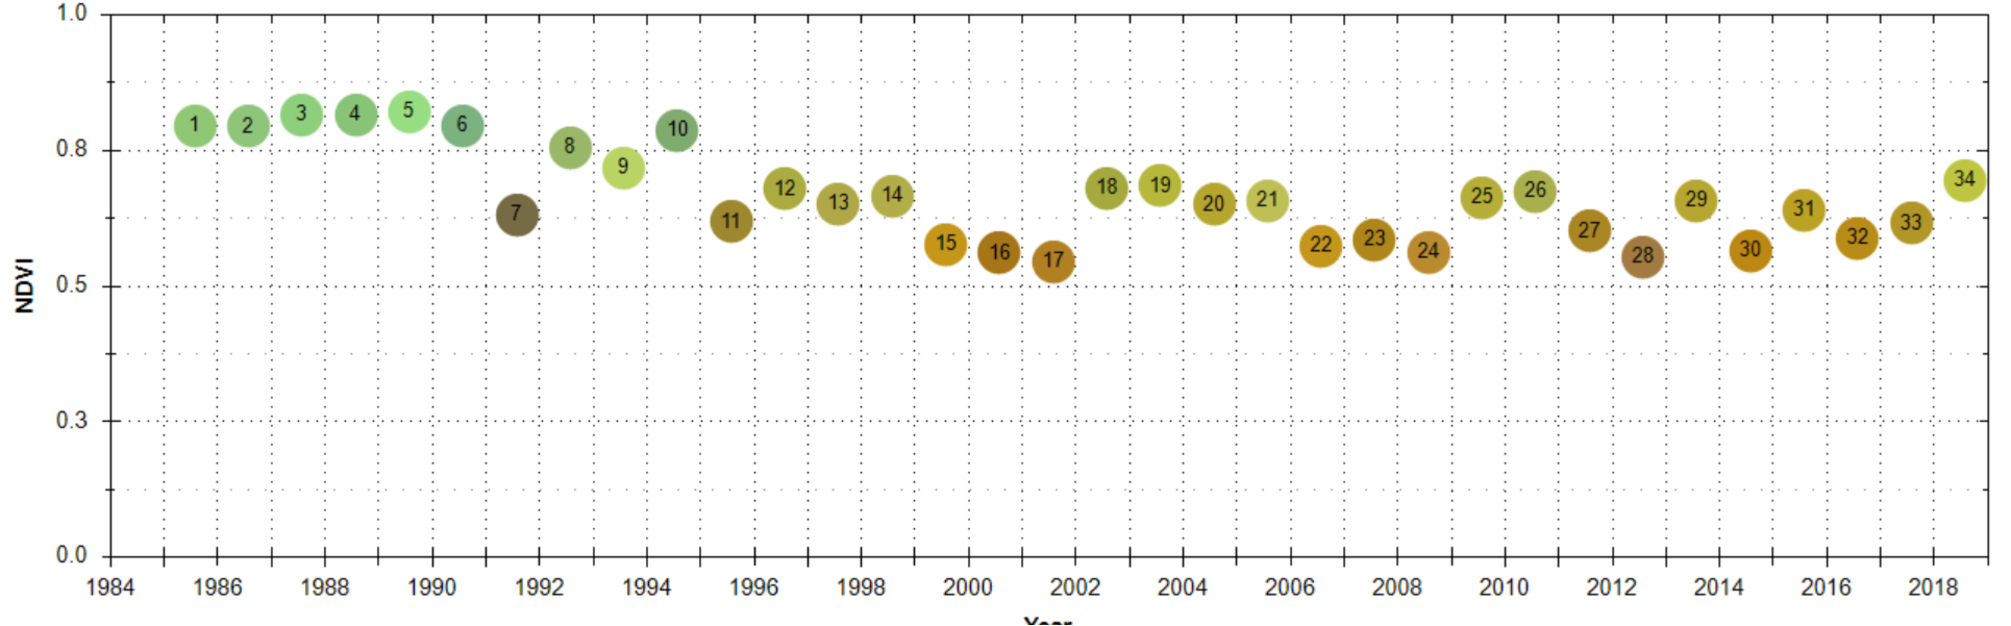
\includegraphics[scale=.4]{images/loss_22_bhrsj_graph.pdf}
    \caption{Visualização dos valores de NDVI para cada ano. A cor dos pontos segue a mesma coloração obtida pelo pixel na imagem, o que ajuda na interpretação visual dos eventos. Na imagem, podemos ver um evento de perda.}
    \label{fig:loss_22_bhrsj_graph}
\end{figure}

\begin{figure}[H]
    \centering
    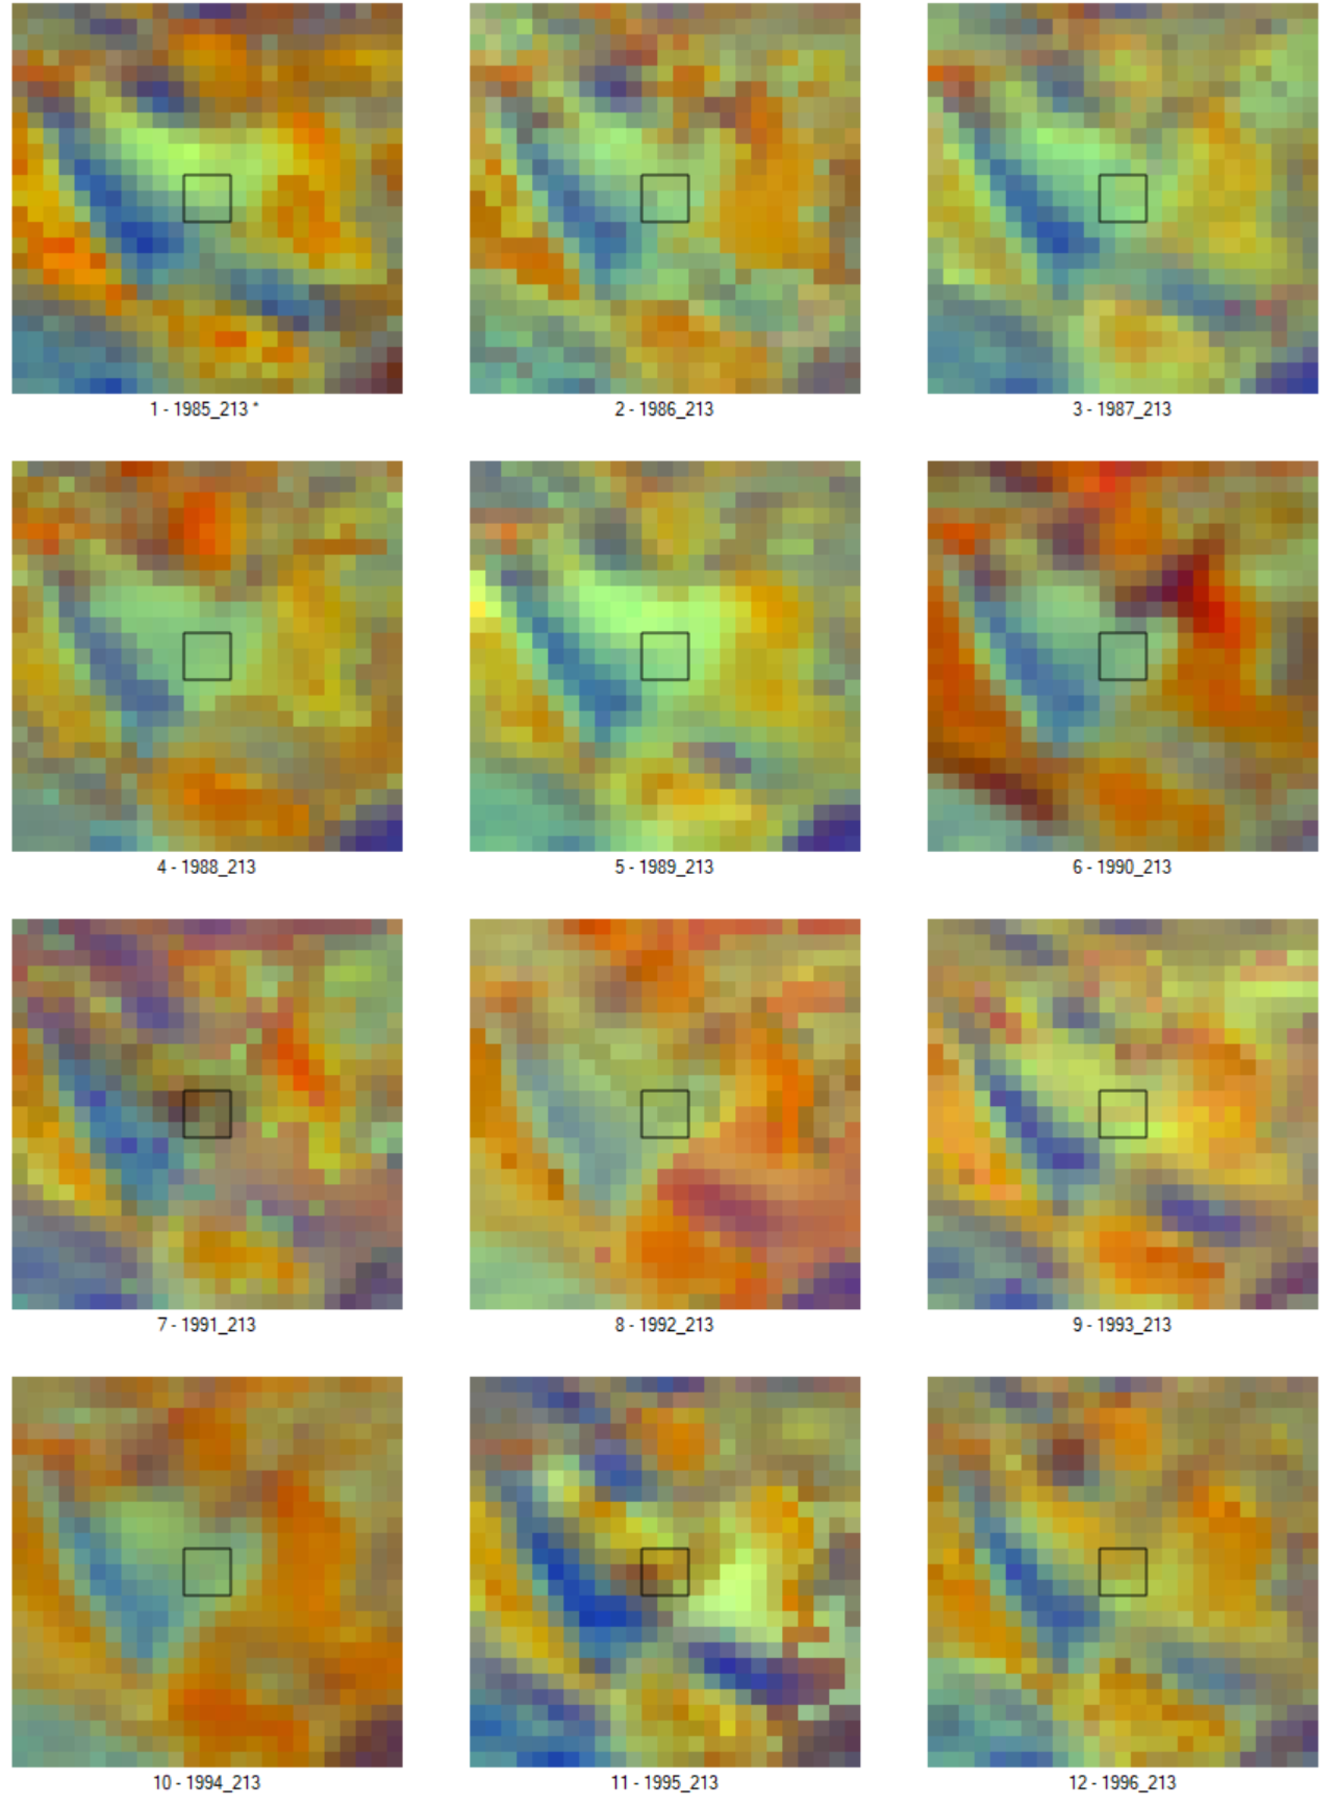
\includegraphics[scale=.5]{images/loss_22_bhrsj_imgs.pdf}
    \caption{TimeSync Image Viewer. Evento de perda na bacia hidrográfica do rio São João. Cada imagem representa o mesmo pixel/local para cada ano do estudo.}
    \label{fig:loss_22_bhrsj_imgs}
\end{figure}

Desde a implementação do Landtrendr no GEE, o TimeSync ainda possui scripts em Python que visam facilitar a exportação de séries temporais do GEE para um ambiente \textit{offline}. Esta etapa é essencial, já que diferente da versão para ENVI/IDL do Landtrendr, no GEE, toda a etapa de preparação dos dados de entrada e de seu processamento são feitos na nuvem de forma quase que automática pelo próprio algoritmo. Como a validação tem de ser feita em ambiente \textit{offline}, é necessário baixar a série inteira ou pedaços da mesma para a realização deste processo. 

No caso da validação de uma área extensa como a da Mata Atlântica, apenas pedaços da série foram exportados já que o processo de exportação de toda a área seria muito demorado, custando algumas horas para a exportação de áreas com apenas algumas centenas de $ km^2 $. Devemos considerar também que a exportação de toda a série para uma área extensa em resolução espacial de 30m necessitaria de excessivo espaço para armazenamento, sendo incoerente com a proposta inicial de processamento de grande escala e com baixo custo. 
Sendo assim, uma área de teste foi escolhida para cada fitofisionomia estudada.

Para cada área selecionada, pontos aleatórios distribuídos de forma estratificada foram gerados para três classes distintas: Ganho, Perda e  pseudo-invariância/Outros. A classe de Pseudo-invariância/Outros foi criada para comportar todos os pontos que na verdade não eram de interesse da análise de detecção de mudanças. Sejam por serem áreas que se mantiveram constante ao longo dos anos estudados ou porque foram mascaradas por serem áreas urbanas, áreas naturais não vegetada ou qualquer outra classe de não interesse. Para cada classe foram gerados 100 pontos, totalizando 300 pontos de validação para cada fitofisionomia, uma soma total de 900 pontos. Além disso, mais 300 pontos (100 por classe) foram validados para a Bacia Hidrográfica do Rio São João com o intuito, assim como no estudo sobre a banda CSNR, verificar possíveis variações no resultado do algoritmo para regiões geograficamente distantes mas fitofisionomicamente similares.

Nas áreas de floresta ombrófila densa, os resultados mostraram uma acurácia de 90\% e um kappa de 0.85. Já nas áreas de vegetação ombrófila mista, obtivemos uma acurácia de 88\% com um kappa de 0.82. Finalmente, nas áreas de vegetação estacional semidecidual, a acurácia, como esperado, foi um pouco menor ficando em 84\% e com kappa 0.76. Apesar da diferença aparente entre regiões ombrófilas e estacionais, todas as regiões obtiveram resultados considerados altos, e portanto, satisfatórios, mostrando que ao utilizar composições anuais essas diferenças causadas pelas dinâmicas estacionais acabem se diluindo. Não foram detectadas diferenças significativas entre os erros de comissão e omissão. As mesmas mantiveram resultados semelhantes em todas as fitofisionomias analisadas.  
Esta diluição causada pela composição de séries anuais fica ainda mais clara quando os testes para a região adicional da Bacia Hidrográfica do Rio São João foram analisados. Para a bacia, uma região classificada como ombrófila densa, foi obtido uma acurácia de 85\% e kappa de 0.77, o que estaria muito mais próximo dos resultados obtidos para a região estacional do que das ombrófilas. Espera-se que os resultados obtidos por fitofisionomia possam contribuir para o entendimento da característica mais homogênea dos estudos que tem como dado de entrada composições derivadas de uma coleção densa de imagens. Além disso, uma validação considerando todas as regiões estudadas foi feita, obtendo um valor de acurácia global de 86.7\% e kappa de 0.8. 

Estes resultados demonstraram um excelente resultado obtido pelo algoritmo e confirmam seu potencial para aplicação em áreas tropicais extensas.

\subsubsection{Plataforma para visualização dos resultados}

\hspace{13pt} Uma das dificuldades encontradas na análise de áreas extensas como a Mata Atlântica está na representação dos resultados, principalmente em escalas derivadas de resoluções espaciais médias como no caso das imagens Landsat. A criação de mapas de calor e criação de estatísticas zonais acabam servindo para uma análise mais geral das regiões e até mesmo em nível de município, mas limita uma análise mais pontual, local.

A plataforma do Google Earth Engine (GEE) disponibiliza a possibilidade de criação de uma interface gráfica através da própria API, possibilitando a publicação de resultados obtidos na plataforma ou de dados externos importados para seu ambiente através da criação de um \textit{website}. Esta funcionalidade possibilita a divulgação interativa de forma prática e rápida de grande quantidade de dados. Sem esta infraestrutura, o compartilhamento dos dados resultantes de análises na plataforma teriam de ser feito de forma tradicional, através do \textit{download} dos dados da plataforma e posterior \textit{upload} em serviços de hospedagem na nuvem. Para dados como os resultados obtidos nesta análise esta opção se mostrou essencial, já que os arquivos resultantes são grandes e demandam poder computacional significativo para uma visualização sem engasgos. 

A criação de uma aplicação web utilizando o GEE pode ser feita de forma relativamente simples através da própria interface gráfica. O desenvolvimento da interface gráfica deve ser realizada utilizando a API JavaScript, que possui documentação extensa no próprio \textit{website} oficial. Os dados que serão visualizados devem estar conectados a sua conta do GEE e compartilhados de forma aberta. Após o link dos dados com a interface, é possível fazer a publicação através do botão "App". A plataforma leva alguns minutos para subir a aplicação final e gerar um link compartilhável Figura (\ref{fig:ltr_gee_ui_atlatic_forest}). 

Neste caso, o código para a aplicação ainda foi registrado na plataforma Zenodo com o objetivo de gerar um DOI (10.5281/zenodo.6481487). O código fonte para a aplicação pode ser acessado aqui: https://github.com/sacridini/ui\_gee\_ltr\_mata\_atlantica. A visualização das principais camadas geradas neste trabalho (perda, perda rápida, perda longa e ganho) podem ser acessadas através deste link: https://elacerda.users.earthengine.app/view/atlantic-forest-landtrendr. 

\begin{figure}[H]
    \centering
    \includegraphics[scale=.3]{images/ltr_gee_ui_atlatic_forest.pdf}
    \caption{Página principal da aplicação web para visualização dos resultados de mudança na Mata Atlântica}
    \label{fig:ltr_gee_ui_atlatic_forest}
\end{figure}

\subsubsection{Resultados para os eventos de perda na Mata Atlântica}

\hspace{13pt} Somando-se todos os eventos de perda detectados pelo algoritmo após as filtragens das áreas de interesse, houveram ao longo de todos os anos da análise 61.167.796 de pixels com uma perda média de magnitude de 225 ou diminuição de 0.225 no índice NDVI. Isso equivale a uma área total de pouco mais de 55 mil $ km^2 $ de florestas que sofreram perdas significativas no bioma e que não foram recuperadas após a supressão.

O resultado mais abrangente envolvendo todos os eventos de perda do bioma pode ser visualizado na (Figura \ref{fig:heat_loss_masked85_maskedgain}). A maior aglomeração de eventos de perda está localizada principalmente entre os estados do Paraná e Santa Catarina e no estado da Bahia. Nos outros estados o mapa de calor mostra uma distribuição mais homogênea dos eventos ao longo do território. 

\begin{figure}[H]
    \centering
    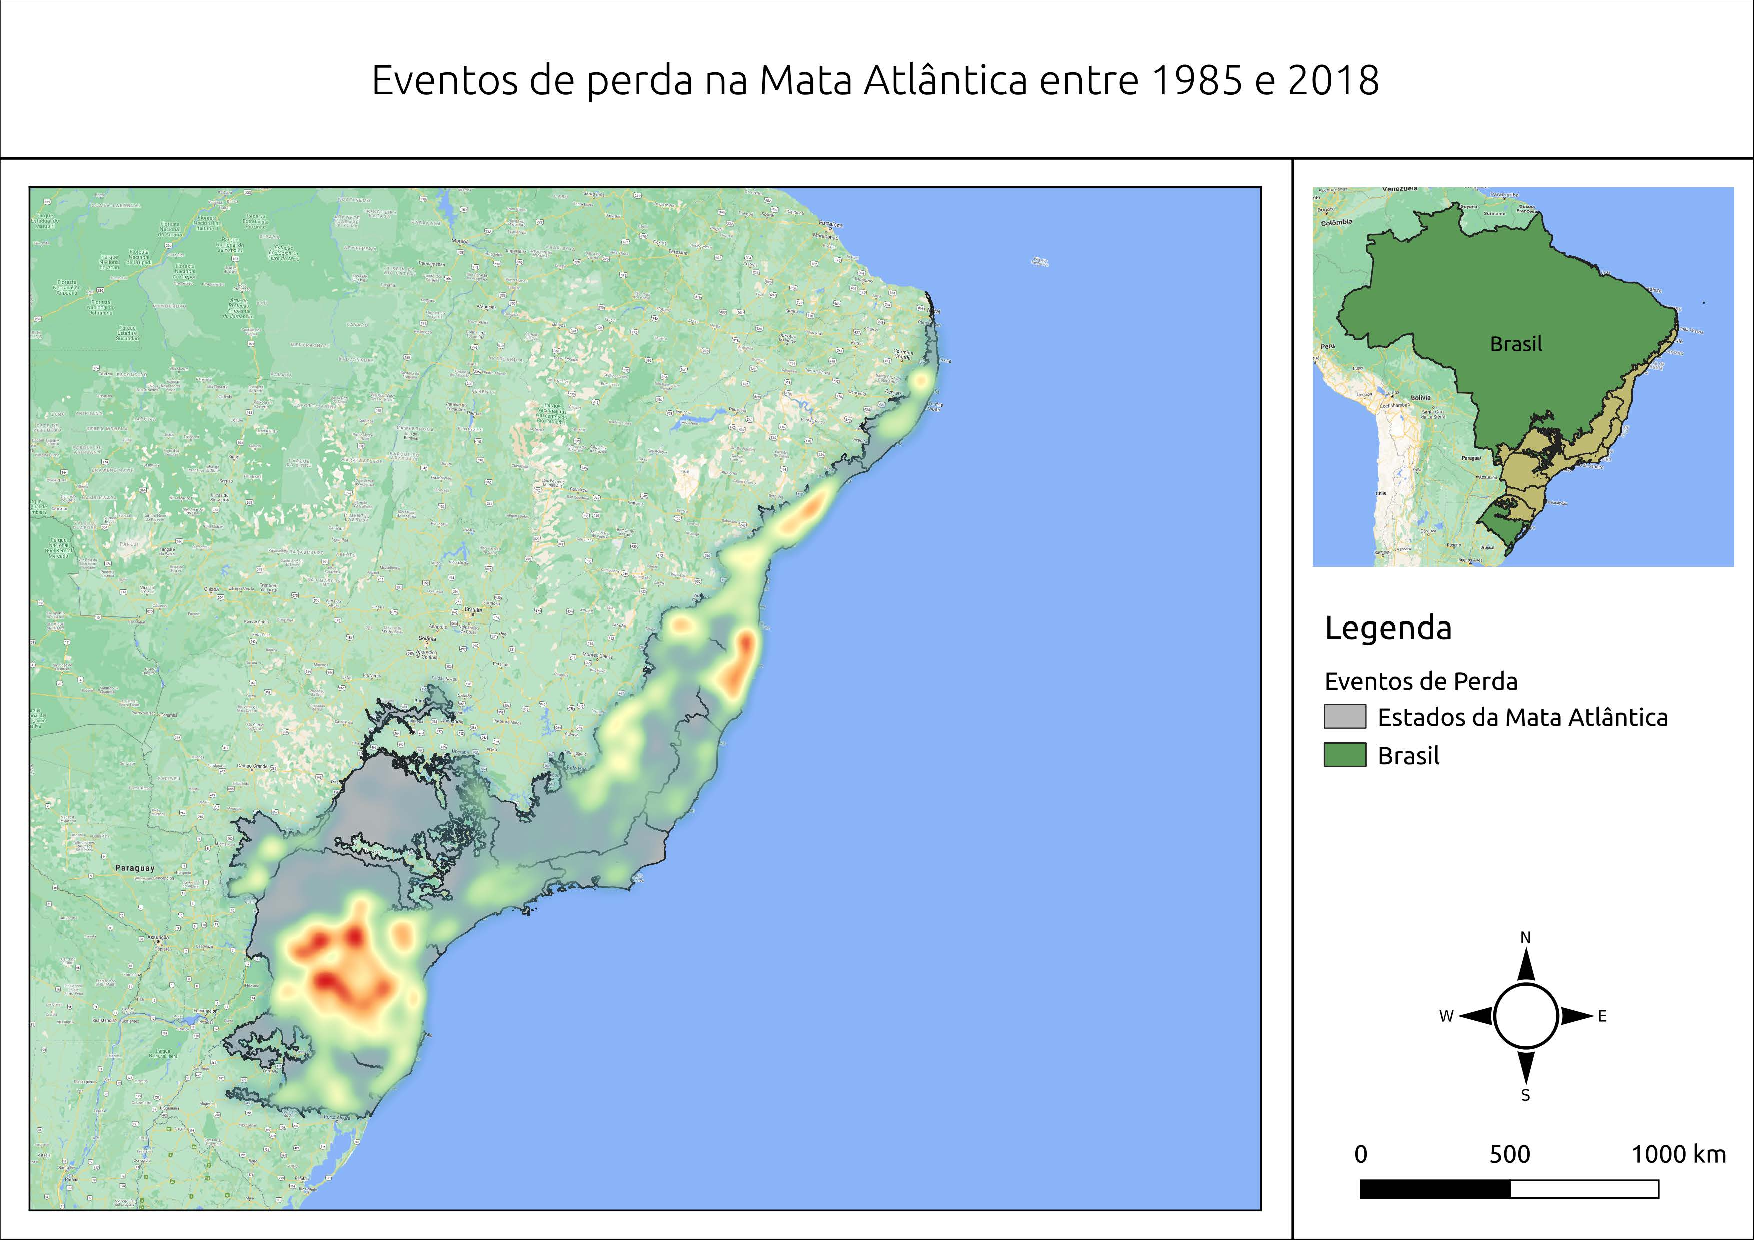
\includegraphics[scale=.5]{images/heatmap_loss_masked85_maskedgain.pdf}
    \caption{Todos os eventos de perda na Mata Atlântica entre 1985 e 2018.}
    \label{fig:heat_loss_masked85_maskedgain}
\end{figure}

\subsubsection{Os eventos de ganho na Mata Atlântica}

\hspace{13pt} Somando-se todos os eventos de ganho detectados pelo algoritmo e após as filtragens necessárias, houveram ao longo de todos os anos da análise 68.869.908 de pixels com um ganho médio de 197 ou aumento de 0.197 no índice NDVI. Isso equivale a uma área total de aproximadamente 62 mil $ km^2 $ de florestas que sofreram ganhos significativos. Como discutido na sessão 3.2.4, áreas de florestas pseudo-invariantes não foram consideradas, sendo assim, esta área representa um ganho real de área verde dentro do bioma. 

Na Figura \ref{fig:heat_gain}, podemos observar que o ganho de áreas no bioma de deu de forma bem mais homogênea que as áreas de perda. Apenas algumas áreas de aglomeração podem ser visualizados como no sul do Rio Grande do Sul, Espírito Santo, sul de Pernambuco, São Paulo e Minas Gerais.

\begin{figure}[H]
    \centering
    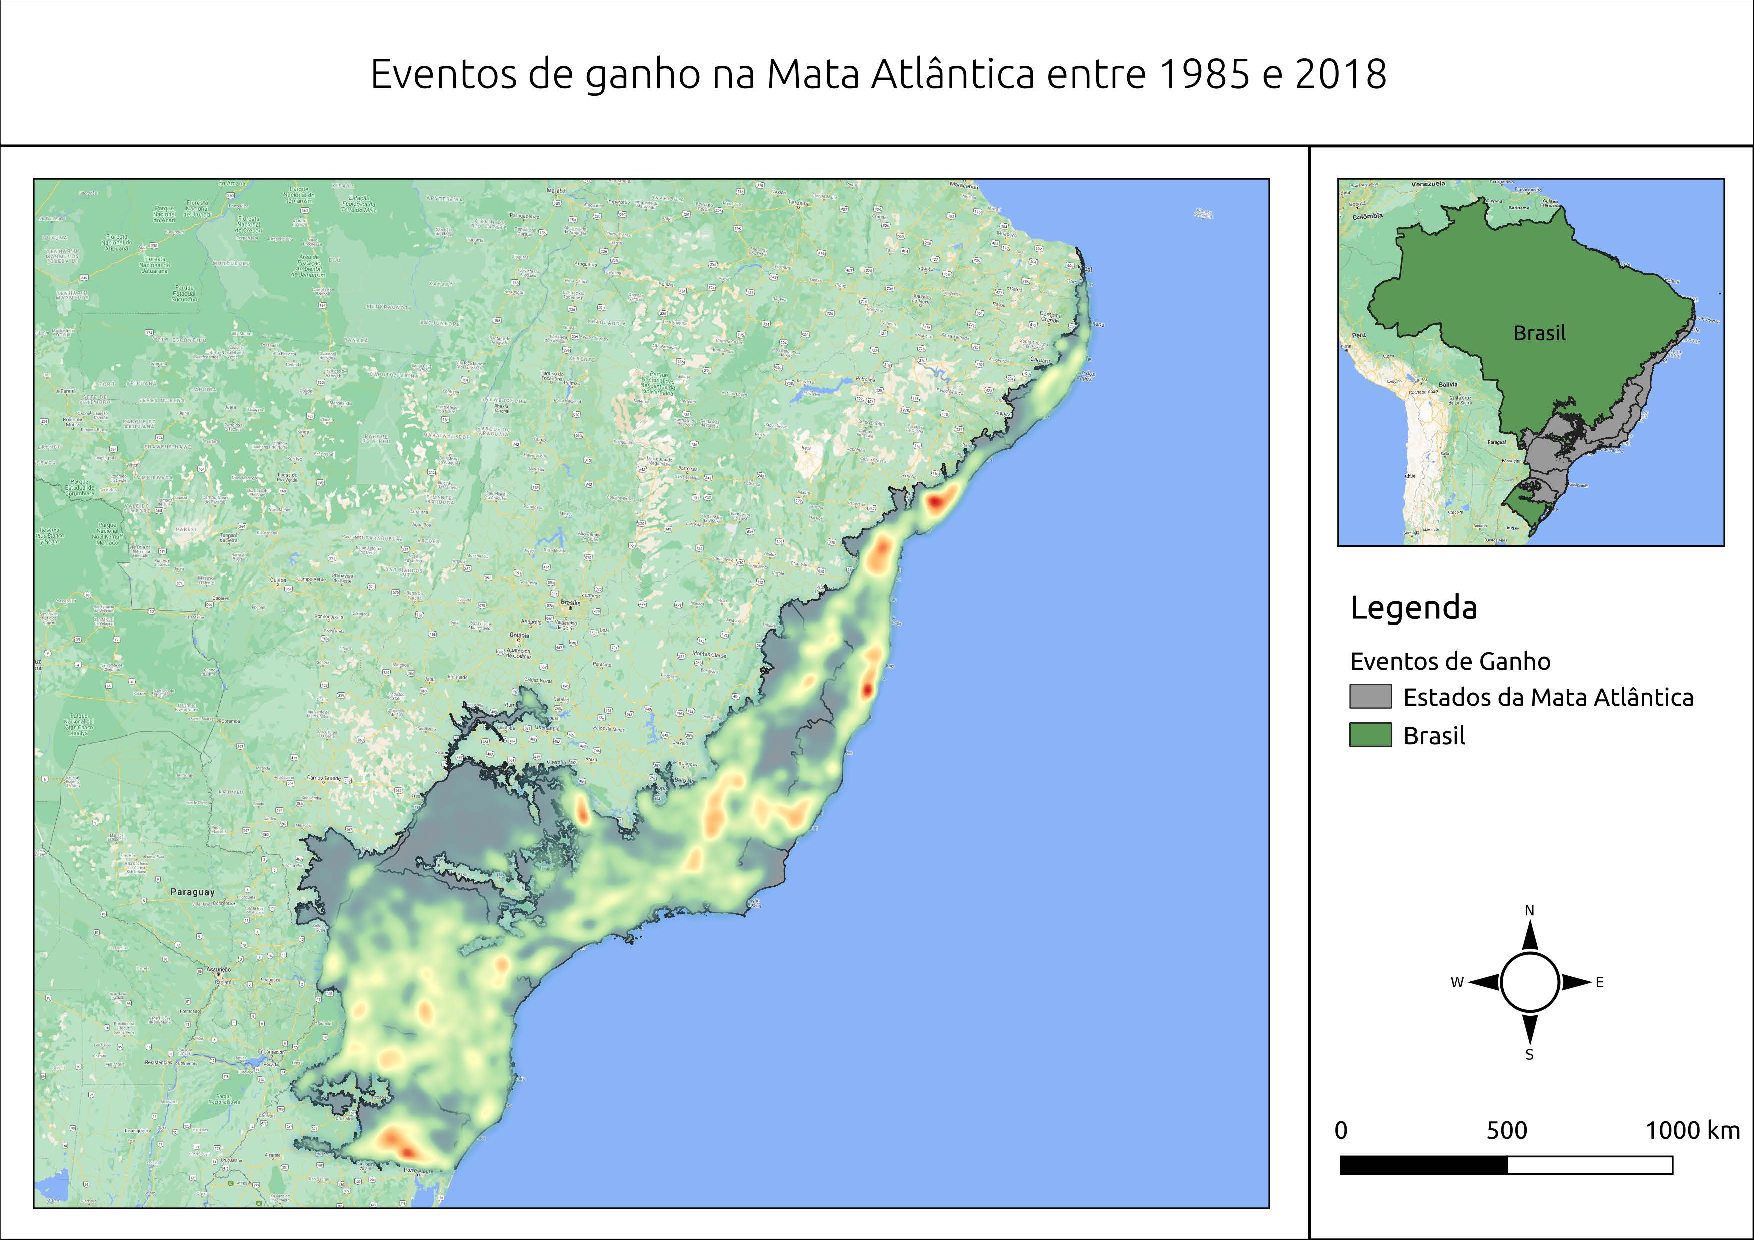
\includegraphics[scale=.5]{images/heatmap_gain_masked18_dur_gt4_inv_for.pdf}
    \caption{Eventos de ganho entre 1985 e 2018.}
    \label{fig:heat_gain}
\end{figure}

\subsection{Conclusão}

\hspace{13pt} Podemos observar através deste estudo que o algoritmo Landtrendr apresentou resultado bastante satisfatório quando aplicado à áreas extensas de floresta tropical. Diferente de estudos realizados anteriormente, foi possível observar o comportamento do algoritmo quando aplicado a diferentes fitofisionomias. Os resultados apresentados são coerentes com os apresentados por programas de mapeamento sistemáticos com o Mapbiomas, mas contribuiu para uma melhor qualificação das mudanças ocorridas no bioma ao longo dos 33 anos da análise. 

Este estudo contribui ainda para o desenvolvimento do conhecimento sobre a aplicação de técnicas de detecção de mudança baseado em trajetórias em um contexto ecológico complexo e fragmentado como o da Mata Atlântica em meso-escala. A incorporação de ferramentas de processamento de dados espacias em infraestruturas computacionais interconectadas demonstra através de trabalhos como este, mais uma vez, sua potencialidade. Não só na clara capacidade extraordinária de processamento como na qualidade das ferramentas disponíveis para análise dos dados. Observando os resultado obtidos, acreditamos que a implementação do Landtrendr para a plataforma Google Earth Engine poderá contribuir para futuras análises, sejam elas locais ou para áreas extensas, utilizando assim todo o potencial de processamento disponível.
% Estes fatores foram essenciais para contarmos esta parte recente e importante da história da Mata Atlântica. 
\newpage


\section{Detecção de Áreas de Florestas Pseudo-Invariantes em Séries Temporais Utilizando Algoritmo Random Forest}

\subsection{Introdução}

\hspace{13pt} O monitoramento remoto da paisagem se estabeleceu em nossa sociedade como uma das principais formas de planejamento estratégico e como uma ferramenta importante para a quantificação de recursos e execução de políticas públicas. Os programas de monitoramento de queimadas e de desmatamento ilegal ganham cada vez mais espaço nos noticiários recentes não somente devido a clara relevância dos resultados obtidos, mas também porque seus resultados repercutem diretamente em muitos dos acordos comerciais que os países tem a possibilidade de realizar. 

Dentre todas as possibilidades de uso de ferramentas de sensoriamento remoto para a detecção de mudanças da paisagem, a detecção de mudanças em áreas florestadas focando em eventos de supressão tem um papel importante e possivelmente é uma das mais estudadas e com maior foco na área. Além dos motivos apontados anteriormente, os dados de monitoramento das supressões ocorridas nessas áreas podem ser usados também como dado de entrada para análises que visam a priorização espacial de áreas estratégicas para a conservação e, mais recentemente, para a restauração de áreas com histórico de supressão. Projetos como o Mapbiomas \citep{Souza2019} realizam o mapeamento sistemático do uso do solo para todo o território nacional e a detecção de mudanças de uso ao longo do período do mapeamento (1985 – 2018), sendo um exemplo de como a área de geotecnologias pode se beneficiar com o aumento do acesso à computação de alto desempenho. 

Além disso, devido a esse aumento do poder computacional e de seu acesso, novos algoritmos visando a análise de séries temporais, utilizando imagens digitais orbitais como base, surgiram como uma tentativa de aprimorar, não só a detecção da mudança em si, assim como de sua interpretação, agregando cada vez mais conteúdo de qualidade às análises. Alguns desses algoritmos visam a detecção de mudanças em áreas de floresta como é o caso do CCDC - Continuous Change Detection and Classification \citep{ZHU2014152}, COLD - Continuous Monitoring of Land Disturbance \citep{Cohen2020}, Landtrendr \citep{KENNEDY20102897, KENNEDY2012117}, VCT – Vegetation Change Tracker \citep{Huang2010, THOMAS201119}, EWMACD - Exponentially Weighted Moving Average Change Detection \citep{Brooks2014}, MIICA - Multi-index Integrated Change Analysis \citep{JIN2013159}, VerDET - Vegetation Regeneration and Disturbance Estimates through Time \citep{Hughes2017}, ITRA - Image Trends from Regression Analysis \citep{VOGELMANN201292} e o Shapes-NBR \citep{Meyer2013, Moisen2016}.

Pensando pela perspectiva temporal, é importante entender exatamente qual tipo de mudança se espera obter com a utilização desses algoritmos. Muitas das ferramentas já citadas possibilitam a detecção não somente de eventos de grande magnitude, mas também de processos de degradação que ocorreram ao longo de décadas, ou seja, processos de baixa magnitude, o que possibilita estudos mais elaborados, mas que ao mesmo tempo podem gerar resultados com mais ruído.

Como se pode imaginar, a limpeza dos dados na etapa de pós processamento desses algoritmos acaba sendo essencial para a obtenção de resultados de boa qualidade. É normal que pequenas variações na própria radiometria da imagem sejam detectadas como mudança. Apesar de ser possível retirar grande parte desse ruído considerando apenas mudanças com magnitudes mais altas, áreas de floresta que possuem alta declividade, por exemplo, tendem a sofrer mais com certos ruídos. Sendo assim, parte da limpeza desses dados normalmente acontece utilizando dados gerados por projetos como o Mapbiomas. Os dados do Mapbiomas podem ser utilizados como uma máscara para ignorar áreas de não interesse. Pixels que foram classificados em todos os anos do mapeamento do Mapbiomas como áreas urbanas, corpos d’água, pasto, solo exposto, agricultura e, claro, florestas, são binarizados e multiplicados entre si (classe a classe) para serem utilizados como máscaras com o objetivo de limpar possíveis ruídos no resultado final de um algoritmo como o Landtrendr \cite{KENNEDY2007370, KENNEDY20102897, Kennedy2018}. No entanto, os mapeamentos anuais do Mapbiomas entendem a classificação de forma anual, e não de forma multitemporal, o que pode implicar em erros quando a multiplicação das classificações é realizada para gerar as camadas binárias que servirão para limpar os ruídos. Um pixel que possa ter sido mapeado de forma equivocada em um único ano pode anular a inclusão desta mesma área como uma área a ser utilizada como máscara. Portanto, ao utilizarmos este método, somente áreas bem consolidadas acabam sendo selecionadas para limpar o resultado gerado pelo algoritmo de detecção de mudança.

Sendo assim, o presente trabalho buscou elaborar uma alternativa a esta técnica, apresentando uma forma mais precisa de gerar camadas de áreas de estabilidade, ou seja, áreas que apesar de terem sido afetadas por pequenas mudanças mantiveram alguma característica principal ao longo da série. O foco dado neste trabalho foi para a classe que chamamos aqui de florestas invariantes, já que normalmente é a classe de maior interesse e possivelmente a que possui maior quantidade de ruído associado. Diferentemente do método mais tradicional, a ideia foi realizar a criação de uma máscara gerada a partir da classificação de toda a série temporal e não da agregação de camadas classificadas individualmente ano a ano. 

\subsection{Metodologia}

\hspace{13pt} Para a realização deste trabalho utilizou-se como área de estudo o limite a APA da Bacia Hidrográfica do Rio São João (Figura \ref{fig:bhrsj}). A área foi escolhida por já possuir extenso número de trabalhos de referência publicados e por apresentar elementos da paisagem que representam de forma geral grande parte o contexto morfoclimático e fitogeográfico do Estado do Rio de Janeiro.

\begin{figure}[h!]
    \centering
    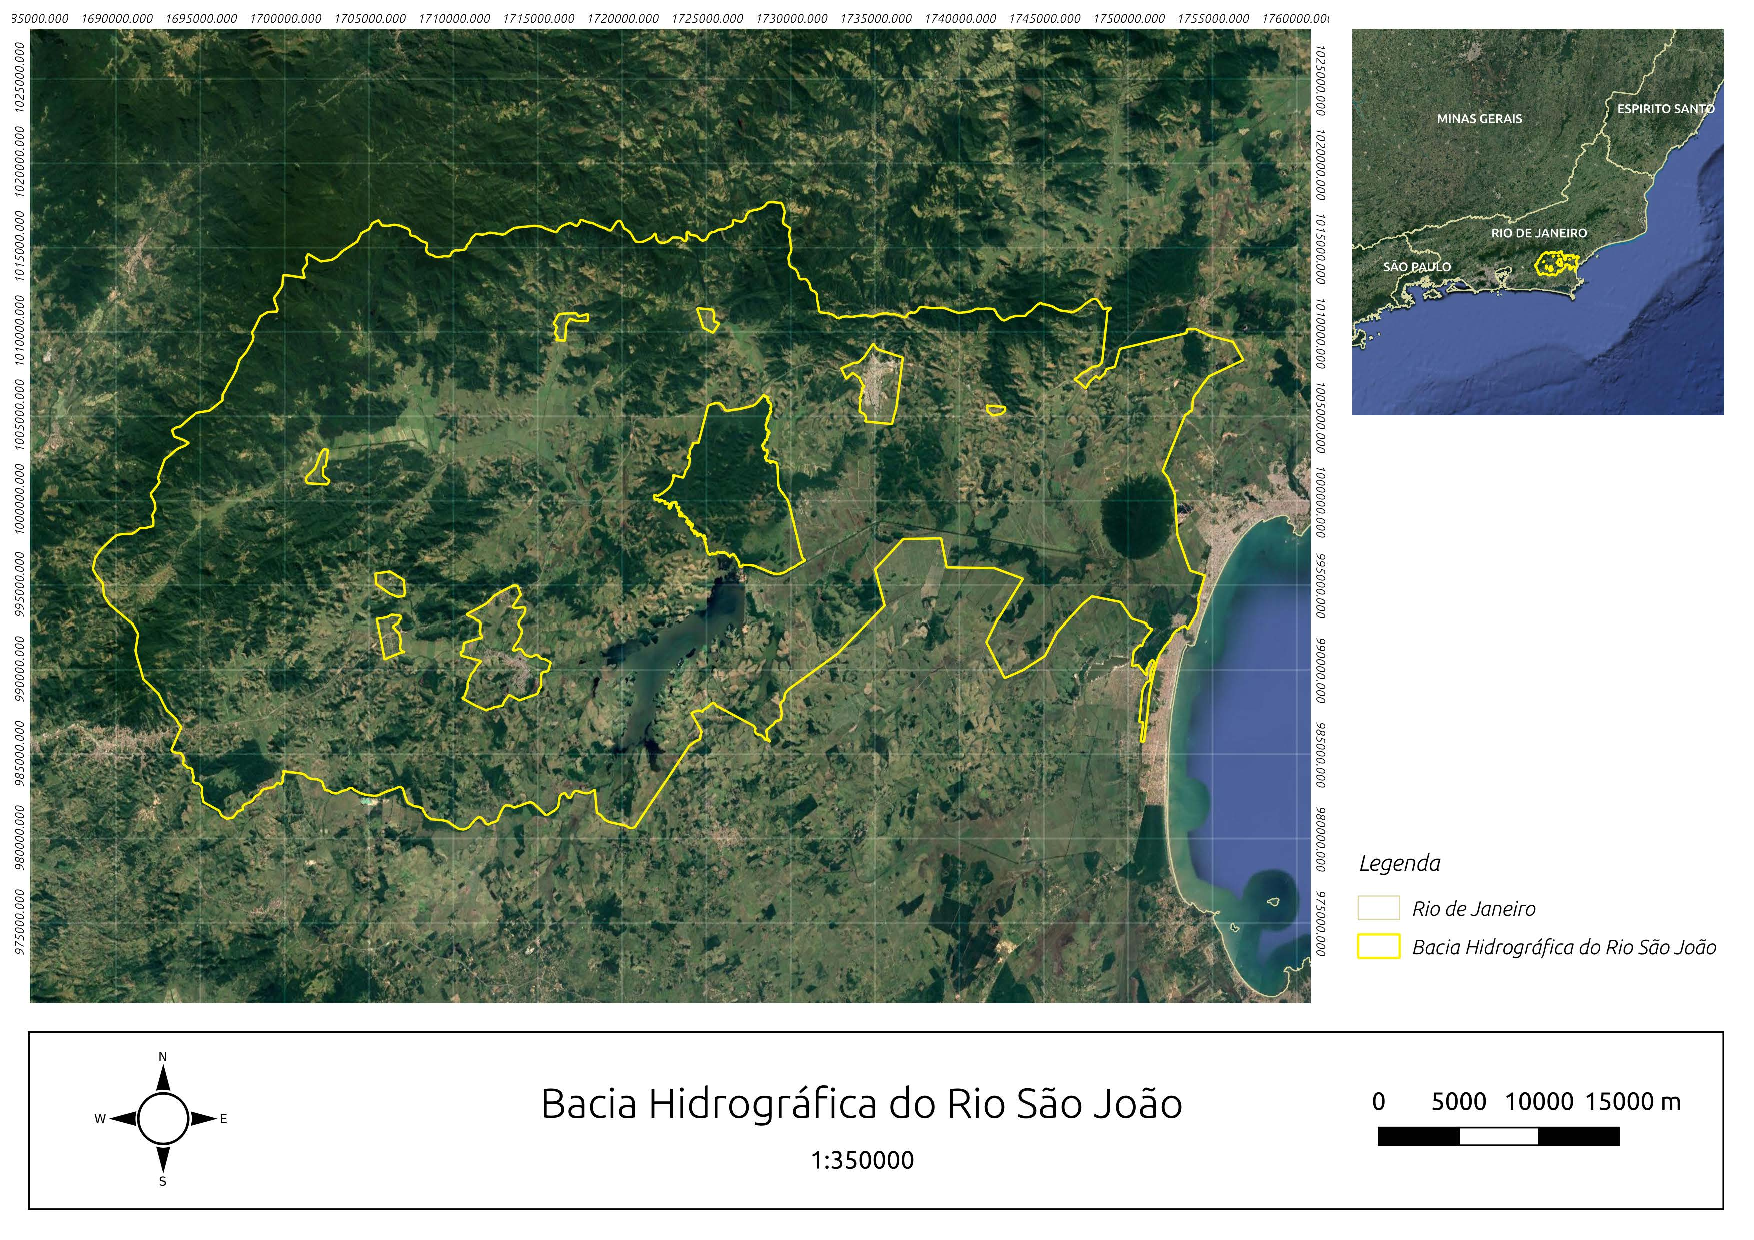
\includegraphics[scale=.5]{images/bhrsj_v2.png}
    \caption{O valor de biomassa chegou a ser ainda menor do que quando a maior perda foi registrada.}
    \label{fig:bhrsj}
\end{figure}

Inicialmente foi necessário gerar a camada de floresta invariante utilizando os dados do Mapbiomas. Ou seja, tudo que foi classificado como floresta durante todos os anos do mapeamento. Neste caso, floresta é tudo que foi classificado como “Formação Florestal” pelo Mapbiomas. Para isso, todas as camadas de uso do solo para o bioma da Mata Atlântica gerados pela série 4.1 do projeto (de 1985 até 2018, totalizando 33 camadas) foram recortados de acordo com os limites da APA e passaram por um processo de reclassificação, resultando em camadas binárias (floresta e não-floresta). Após a reclassificação, todas as camadas foram multiplicadas entre si resultando finalmente em uma camada binária final, onde florestas possuem com valor 1 e áreas de não-floresta valor 0.

Como a proposta metodológica consiste na aplicação de um algoritmo de classificação em toda a série temporal, foi essencial a coleta de boas amostras representativas de florestas invariantes. Boas amostras são essenciais para um resultado final satisfatório. Além disso, não seria prudente utilizar somente a camada do Mapbiomas para coletar tais amostras, já que a mesma seria posteriormente comparada com o resultado final. Sendo assim, além da utilização dos próprios dados do Mapbiomas, foi gerada uma imagem sintética do valor máximo de NDVI, considerando todos os anos da série temporal, de forma a realizar uma coleta de amostras através de uma abordagem mais conservadora.

A camada de máximo valor de NDVI foi toda desenvolvida utilizando a plataforma GEE. Para a geração dessa camada foram utilizadas todas as imagens disponíveis do satélite Landsat considerando as séries 5, 7 e 8. Foram utilizadas todas as imagens disponíveis para todos os três satélites presentes na coleção Surface Reflectance Tier 1 por já possuírem correção atmosférica (6S).

Após uma filtragem inicial, aplicou-se uma função em cada uma das imagens (datas) disponíveis, gerando-se uma imagem NDVI correspondente. Através de uma outra função retirou-se todos os pixels com presença de nuvens e sombras.

Com o conjunto total de imagens NDVI, extraiu-se para cada ano da série a mediana dos valores obtidos por pixel e, a partir do novo conjunto gerado, extraiu-se o valor máximo encontrado em toda a série. Desta forma, a camada final representou o valor máximo das medianas de cada ano. A escolha da mediana como um passo intermediário foi crucial para a eliminação de ruídos e valores inválidos presentes na série temporal, dado que o cálculo baseado apenas na extração dos valores máximos gera uma camada final com ruídos espalhados por toda a imagem.

Após a criação da camada de máximo valor de NDVI, buscou-se um limiar para o valor de corte do que poderíamos classificar como floresta. Considerando que os tipos de uso do solo que mais podem gerar confusão em uma classificação com áreas de floresta são as áreas de pastagem e agricultura, uma nova camada contendo somente essas duas classes foi gerada utilizando os mesmos dados do Mapbiomas com a mesma metodologia realizada anteriormente para as áreas de floresta.

Tanto a camada raster de florestas invariantes (Mapbiomas) como a de pasto/agricultura invariantes (Mapbiomas) foram transformadas em pontos (vetor), selecionando-se dois mil destes pontos de forma aleatória para a aplicação de um teste t de Student. A seleção de pontos de forma aleatória se deu desta forma para evitar um possível enviesamento espacial. A aplicação do teste t de Student resultou em um valor-p de 2.2e-16, apresentando, portanto, diferença significativa entre as duas amostras. Com isso é possível concluir que as amostras com os valores de NDVI de florestas tem alta chance de pertencerem a áreas de floresta. Sendo assim, uma função para extrair o valor mínimo presente nas duas mil amostras de florestas foi processada apresentando um valor de 0,83. O valor de 0,83 pode então ser utilizado como valor de limiar de corte (threshold) para a geração de camadas binárias. A multiplicação da camada binária de florestas invariantes do Mapbiomas com a camada binária de máximo NDVI (todos valores maiores que 0.83) serviu então como nossa camada para extração de pontos de floresta para o treinamento do modelo de classificação.

Já para a extração de pontos de florestas que apresentaram alguma mudança significativa, utilizou-se o resultado do algoritmo Landtrendr. A escolha deste algoritmo se deu à sua capacidade de detecção de eventos de baixa magnitude, o que em muitos casos significa a detecção de processos de degradação mais lentos e longos além claro da típica detecção de eventos de grande mudança. Dentre os muitos resultados que o algoritmo oferece, a camada escolhida foi o da detecção dos maiores eventos de perda de vegetação (Greatest Loss) utilizando imagens anuais de 1985 até 2018 e considerando todas as imagens disponíveis para cada ano no período de 1 de janeiro até 31 de dezembro. Como camada padrão utilizou-se o NDVI para o processamento do resultado final.

Após o Landtrendr apresentar o resultado com todas as maiores perdas detectadas, iniciou-se o processo de limpeza desses dados ao considerar apenas as mudanças com magnitudes maiores que 200, ou seja, perdas maiores que 0,2 no NDVI em um único evento. Nenhuma outra limitação foi imposta ao algoritmo e todos os outros parâmetros foram utilizados de forma padrão sem nenhuma modificação.

Já os pontos para a classe “outros” (água, solo exposto, pasto, etc.) foram coletados de forma aleatória utilizando a imagem resultante com todos os pixels que não tinham sido classificados anteriormente nem como floresta pela fusão da camada do Mapbiomas com o NDVI máximo, e nem pelos pixels detectados pelo Landtrendr como áreas com possível perda de vegetação.

Todas as amostras das três classes foram então importadas em formato shapefile para a plataforma do Google Earth Engine (GEE) para execução do processo de classificação utilizando o algoritmo Random Forest. Como imagem base para a classificação foi necessário ter uma série temporal com imagens anuais seguindo os mesmos padrões da série do Mapbiomas para possibilitar posterior comparação. Essa série de imagens foi gerada utilizando um script desenvolvido no GEE contendo, para cada ano, uma composição de valores considerando o valor da mediana de cada pixel para cada banda. Para cada ano foram utilizadas as bandas Blue, Green, Red, NIR, SWIR1, SWIR2 e também de índices como o NDVI, NDWI, NDMI, SAVI, Greenness, Wetness e Brightness. Áreas com nuvens e sombra foram mascaradas com valores “no data” e, portanto, não foram consideradas no cálculo da mediana.

No entanto, por se tratar de uma nova metodologia, antes de gerar o processo de classificação final utilizando as amostras coletadas, escolhemos realizar testes de validação cruzada (cross validation) para entender melhor quais variáveis (bandas) teriam o melhor desempenho ao classificar este tipo de classe. Utilizamos então as amostras coletadas (250 pontos/classe) para extrair os valores da série temporal e exportamos para um ambiente offline, já que atualmente não existem ferramentas de teste e validação suficientemente boas no GEE.

As tabelas com os valores das amostras foram processadas no pacote MLR (Machine Learning in R) (BISCHL, et al., 2016) utilizando o classificador Random Forest com 100 árvores cada e com a validação cruzada em modo “k-fold” utilizando parâmetro 10 (divide o subconjunto das amostras em 90\% treino e 10\% teste), repetindo ainda o processo por 100 iterações para cada teste, obtendo então um único valor de índice kappa por teste. Cada rodada aqui representa uma combinação de bandas a serem utilizadas pelo classificador para tentar separar as três classes. Para este teste foram consideradas 24 combinações diferentes de bandas. Aplicando o Random Forest para as 24 variações de entrada com o processo de validação cruzada utilizando 10 “folds” e 100 iterações para cada validação, foram gerados 24000 processos de classificação diferentes, com cada processo gerando 100 árvores de decisão (Figura \ref{fig:fluxograma}). Os resultados para essa quantidade exaustiva de testes são os apresentados na Tabela \ref{tab:1}:


\begin{table}[h!]
\centering
\rowcolors{2}{red!50!yellow!30}{green!40!yellow!10}
\footnotesize
\begin{tabular}{|c | c|}
\hline
                                                               BANDA &  Kappa \\
\hline
    Blue + Green + Red + NIR + SW1 + SW2 + NDVI + NDWI + NDMI + SAVI &  0.844754 \\
Blue + Green + Red + NIR + SW1 + SW2 + NDVI, NDWI + NDMI + SAVI + TC &  0.839872 \\
                                Blue + Green + Red + NIR + SW1 + SW2 &  0.838804 \\
                                            Blue + Green + Red + NIR &  0.833381 \\
                                                  Blue + Green + Red &  0.832774 \\
         Greeness + Wetness + Brightness + NDVI + NDWI + NDMI + SAVI &  0.829503 \\
                                                   NDVI + NIR + NDMI &  0.819875 \\
                                                          NDVI + NIR &  0.819833 \\
                                     Greeness + Wetness + Brightness &  0.812621 \\
                                                                 Red &  0.812496 \\
                                                               SWIR2 &  0.808915 \\
                                                              Green  &  0.805528 \\
                                                                Blue &  0.800079 \\
                                           NDVI + NDWI + NDMI + SAVI &  0.796679 \\
                                                         NDVI + NDMI &  0.783342 \\
                                                               SWIR1 &  0.778846 \\
                                                             Wetness &  0.767554 \\
                                                           Greenness &  0.761319 \\
                                                               NDVI  &  0.755475 \\
                                                                SAVI &  0.755282 \\
                                                          Brightness &  0.715955 \\
                                                                NDMI &  0.706022 \\
                                                                NDWI &  0.634395 \\
                                                                 NIR &  0.576071 \\
\hline
\end{tabular}
\caption{Índice Kappa para as Combinações de Variáveis Utilizadas. (SW1 = SWIR1, SW2 = SWIR2, TC = Tasseled Cap = Greeness, Wetness, Brightness)}
\label{tab:1}
\end{table}

\newpage

\begin{figure}[h!]
    \centering
    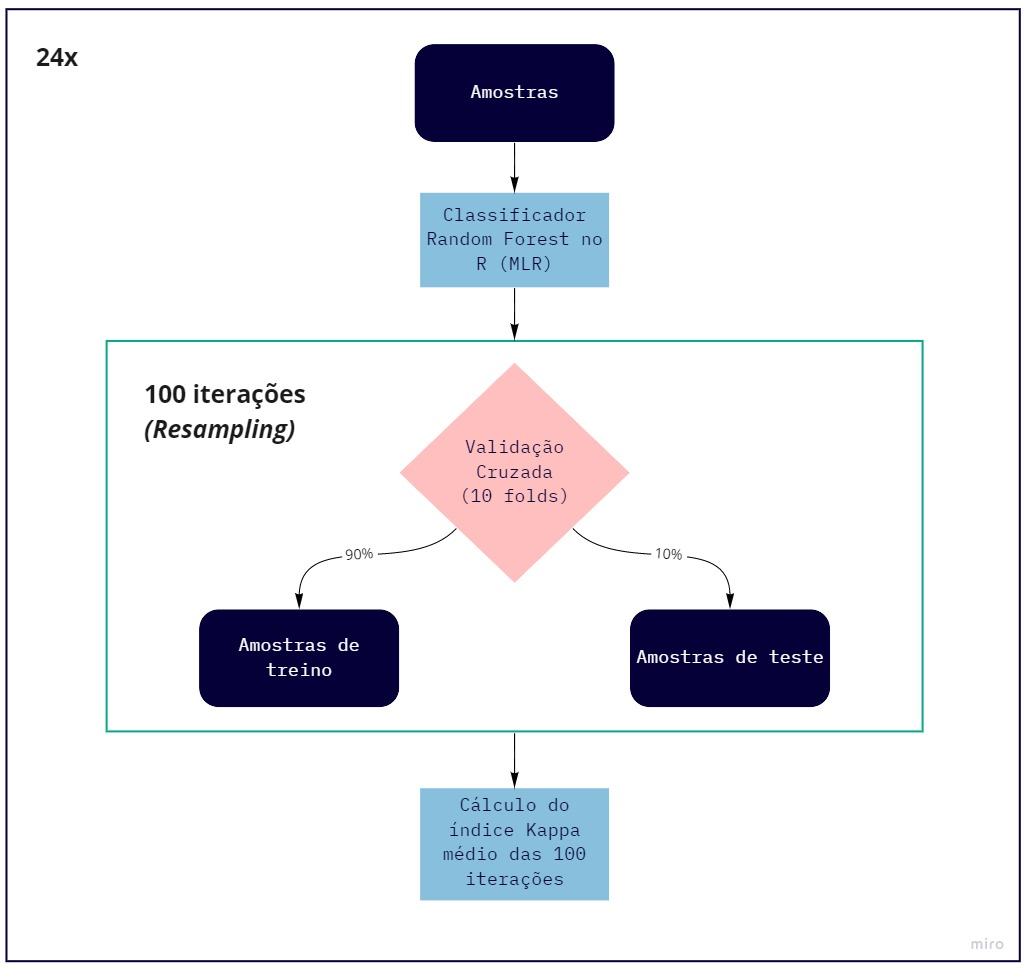
\includegraphics[scale=.4]{images/fluxograma.jpg}
    \caption{Fluxograma demonstrando o processo de validação cruzada. Todo o processo foi repetido para cada combinação de banda utilizada no estudo, totalizando 24 processos independentes.}
    \label{fig:fluxograma}
\end{figure}

É importante frisar que o processo de validação cruzada representa apenas uma etapa intermediária antes da classificação final que visa uma melhor escolha dos parâmetros ao verificar através de muitos testes qual combinação de variáveis obteve melhor resultado (menor erro).

Observa-se que a melhor combinação de bandas para o processo de classificação não é a simples utilização de todas as bandas. A incorporação do Tasseled Cap não trouxe uma melhoria na precisão do modelo. No entanto, a tabela de desempenho também apresenta outros resultados interessantes, como por exemplo a taxa de acerto utilizando apenas a banda do vermelho (Red) ou em como bandas que são tipicamente usadas pela comunidade de forma ampla para detecção de áreas vegetadas como o NDVI, NDMI e SAVI apresentaram resultados piores do que muitas outras combinações possíveis. 

\subsection{Resultados}

\hspace{13pt} Após a otimização do modelo, foi feita uma seleção na série temporal para utilizar apenas a combinação de bandas que obtiveram o melhor resultado (Blue, Green, Red, NIR, SWIR1, SWIR2, NDVI, NDMI, NDWI e SAVI) e assim gerar uma classificação final (Figura \ref{fig:bhrsj_class_final}). Como resultado obtivemos uma área total de florestas invariantes na APA, de 501,1km2.

\begin{figure}[h!]
    \centering
    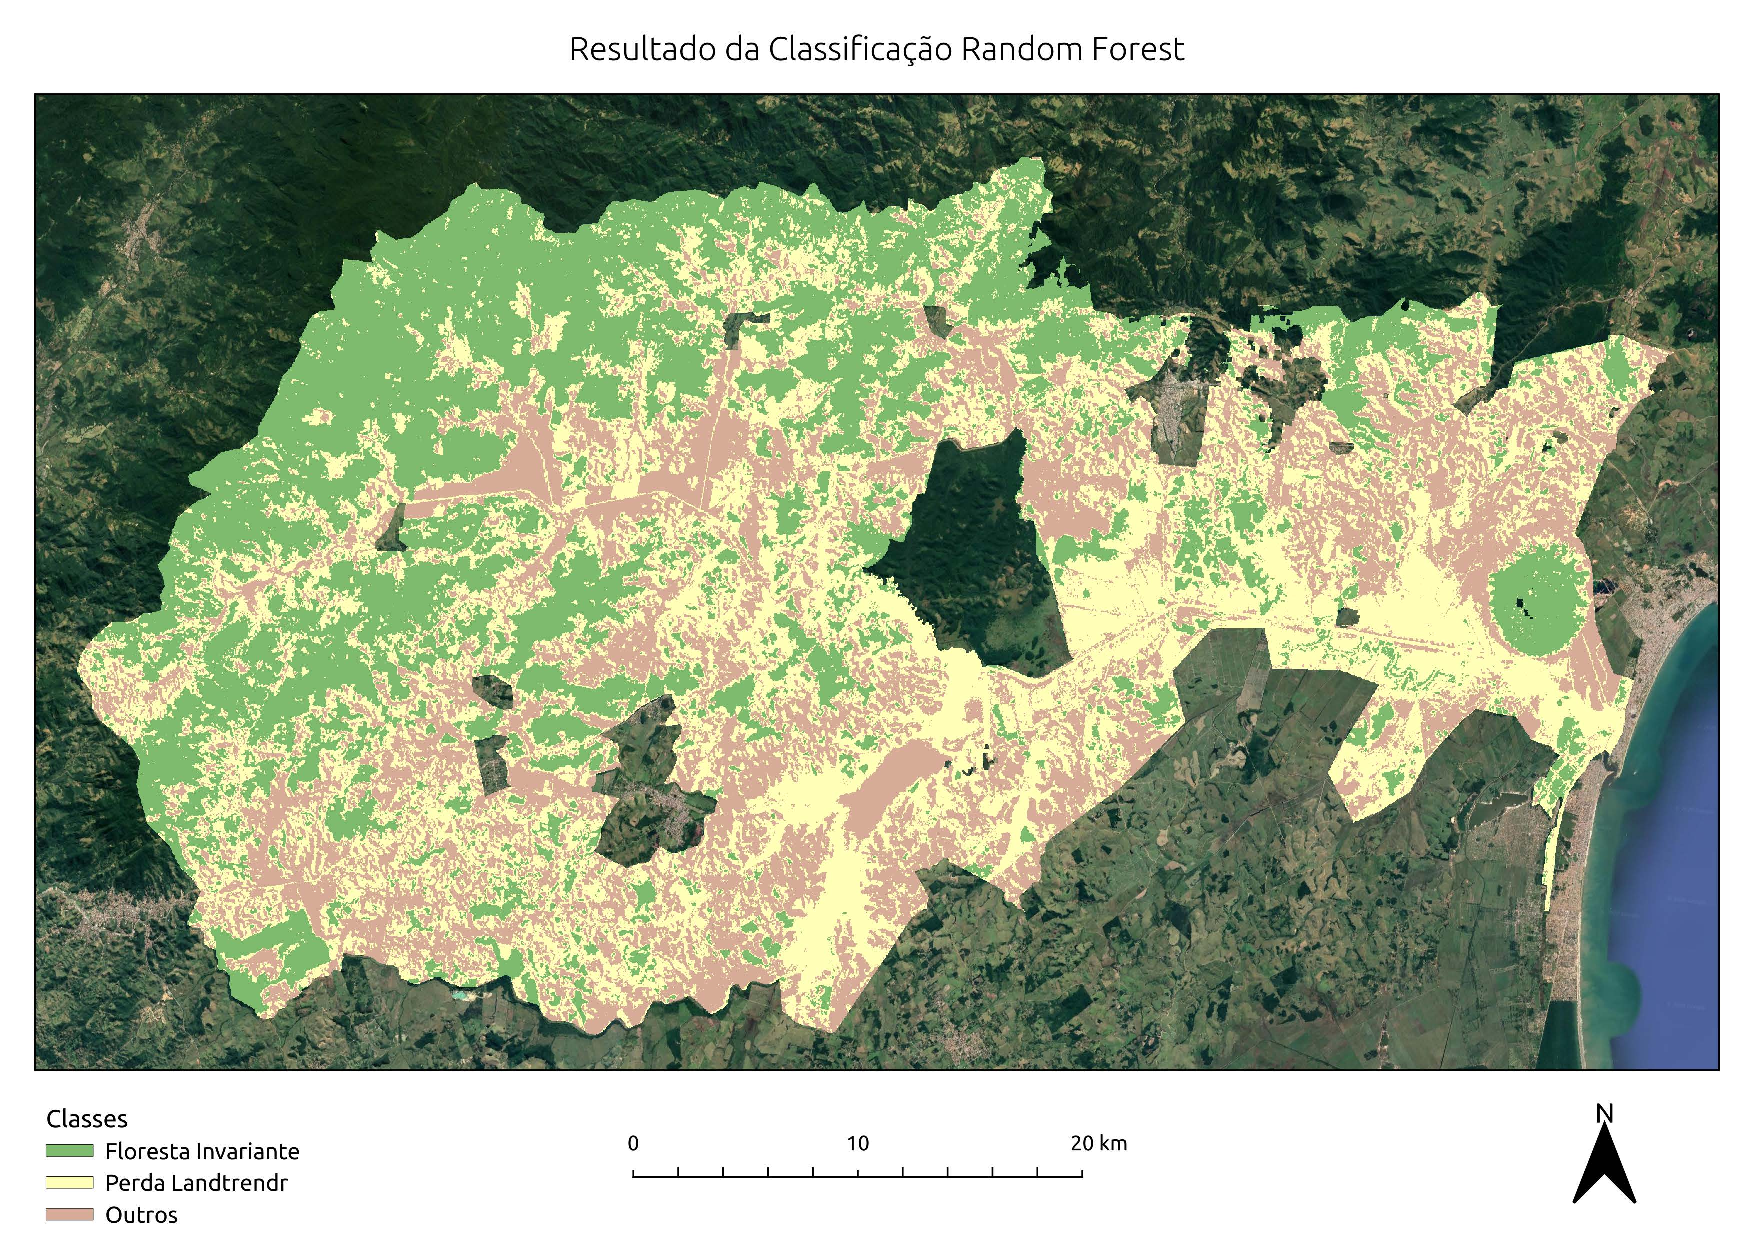
\includegraphics[scale=.5]{images/bhrsj_class_final.png}
    \caption{Classificação final gerada no Google Earth Engine (Classificação final)}
    \label{fig:bhrsj_class_final}
\end{figure}

\newpage

As classes escolhidas para o mapeamento final foram “Floresta Invariante”, “Perda Landtrendr” e “Outros”. A classe “Floresta Invariante” representa todos os pixels que mantiveram algum grau de coerência espectral ao longo da série temporal. Mesmo com algumas variações ao longo do tempo, o classificador pode encontrar padrões e descartar anomalias da série. Este comportamento é importante justamente para descartar ruídos presentes em qualquer série temporal sem a necessidade da aplicação de outros algoritmos de pré-processamento e por já garantir um bom resultado. Já a classe “Perdas Landtrendr” foi fortemente influenciada pelo resultado do algoritmo Landtrendr que já tinha detectado os padrões de perda (loss) anteriormente. Ou seja, é importante garantir que o resultado do algoritmo de detecção de mudanças seja o melhor possível modificando seus parâmetros de acordo com a área de estudo. Por fim, a classe “Outros” representa todas as outras classes presentes na bacia e que foram agregadas para não gerar confusão com os objetivos do mapeamento. O resultado da classificação final foi bastante satisfatório, apresentando um padrão espacial das classes esperado para a área de estudo.

No entanto, além da classificação gerada, uma nova imagem teve de ser criada para a comparação entre o resultado obtido pelo Random Forest e a imagem binária utilizando somente dados do Mapbiomas. A nova imagem foi criada somando-se a camada de florestas invariantes com todos os anos do Mapbiomas com a versão binarizada do resultado final (florestas invariantes - outros).

Com essa imagem fusionada pode se notar que grande parte dos pixels (469,8km2 ou 76,9\% da área mapeada) foram classificados como floresta invariante tanto pelo Random Forest como pelo Mapbiomas. No entanto, diferenças como áreas onde somente o Random Forest classificou como floresta (22,7km2 ou 3,8\% da área mapeada) e onde somente o Mapbiomas classificou como floresta (52,7km2 ou 8,7\% da área mapeada) também foram detectadas. Os outros 10,8\% de área restantes foram excluídos da análise por não serem áreas de interesse.

Para entender melhor a qualidade de cada resultado, foram feitos alguns testes estatísticos. Primeiramente, foram selecionadas duas mil amostras aleatórias de três classes: Áreas que foram classificadas como floresta pelos dois mapeamentos (FOR), áreas que foram classificadas como floresta apenas pelo Random Forest (RF) e áreas que foram classificadas como floresta apenas pelo Mapbiomas (MB). Um teste de análise de variância (ANOVA) foi realizado para entender se os valores encontrados por cada amostra eram estatisticamente similares. O valor-p obtido pela ANOVA foi de 0,0116, o que mostrava uma diferença significativa entre as amostras considerando um limiar de valor-p de 0,05. Sendo assim, buscou-se então realizar um teste entre cada uma das amostras utilizando o teste de Tukey \citep{Tukey1949}. Os resultados são os apresentados na Tabela 2.

\begin{table}[h!]
    \centering
    \begin{tabular}{|c | c|}
    Combinação (Teste de Tukey) &  Valor-p      \\
                Mapbiomas - FOR &  8.489000e-04 \\
                       RF - FOR &  1.841643e-01 \\
                 RF - Mapbiomas &  2.000000e-07 \\
    \end{tabular}
    \caption{Resultados do Teste de Tukey}
    \label{tab:2}
\end{table}

Os resultados foram considerados promissores. Segundo o teste de Tukey, ao mesmo tempo em que as amostras que somente o Mapbiomas mapeou como floresta invariante são significativamente diferentes das que ambos os mapeamentos mapearam como floresta invariante. Já as amostras do Random Forest que são diferente das do Mapbiomas, quando comparadas com as mapeadas por ambos, são estatisticamente similares.

Este resultado mostra que a classificação feita pela metodologia proposta apresenta um resultado possivelmente superior a obtida utilizando somente as camadas do Mapbiomas. No entanto, ainda seria preciso saber o quanto de erro associado poderia existir, não apenas nas áreas mapeadas pelo Mapbiomas ou pelo Random Forest, mas também nas áreas em que ambos obtiveram o mesmo resultado.

Para este processo de validação final utilizamos a ferramenta TimeSync \citep{COHEN20102911}. Diferente do processo de validação comum nos mapeamentos de apenas uma ou poucas datas, a validação de séries temporais densas necessita de ferramentas especiais como o TimeSync, que apesar de ter utilização ainda consideravelmente complexa, é uma das únicas ferramentas existentes que realizam esse tipo de validação. 

O TimeSync funciona de forma integrada com o GEE e também necessita do software Access da Microsoft para armazenar as coordenadas de cada ponto a ser validado. A validação do TimeSync é feita de forma visual através da interface gráfica do programa.

Foram coletados para a etapa de validação no TimeSync trezentos pontos para cada uma das classes. Os pixels mapeados apenas pelo Mapbiomas tiveram uma taxa de acerto de 55\%, enquanto os pixels mapeados pelo Random Forest tiveram uma taxa de acerto de 76\%. Já os pixels mapeados por ambos tiveram um acerto de 97\%. Logo após, um último teste foi realizado considerando outras trezentas amostras do mapa final gerado pela nova metodologia, mas considerando apenas os pixels que foram classificados como floresta invariante, resultado em uma taxa de acerto final de 91,7\%. Todos os resultados, amostras, imagens, arquivos vetoriais, códigos e materiais para validação utilizados neste trabalho estão disponíveis para visualização e possível replicação através deste link: https://github.com/sacridini/florestas\_invariantes\_random\_forest.

\subsection{Conclusões}

\hspace{13pt} Através dos testes realizados neste trabalho podemos verificar que a metodologia proposta apresentou melhor desempenho se comparada à utilização da base de dados do Mapbiomas, quando o objetivo é gerar camadas de florestas que não sofreram nenhuma ou pouca variação ao longo de tempo. É importante lembrar que o Mapbiomas continua sendo uma excelente referência para estudos envolvendo séries temporais, e que a comparação feita visa obter resultados melhores para uma classe que não é oficialmente mapeada pelo projeto já que o mesmo possui objetivos distintos. Os resultados obtidos poderão ser utilizados como base para outros mapeamentos de áreas florestadas invariantes em ambientes tropicais. O trabalho buscou também contribuir para um melhor entendimento das variáveis que melhor conseguem separar classes tão novas como a proposta, já que ainda são poucos os trabalhos que buscam classificar séries temporais nessa escala. Além disso, resultados surpreendentes como o desempenho da banda do vermelho mostram que a utilização de apenas uma única banda pode ser o suficiente para a identificação de áreas similares e servem como um estímulo a novos estudos que visem a detecção de áreas invariantes de forma rápida e pouco custosa.

Máscaras de áreas invariantes como a gerada pelo algoritmo de aprendizado de máquina poderão servir, não só como parâmetros para estudos aplicados à conservação, mas também como máscaras para a limpeza de dados indesejados em resultados obtidos por algoritmos de detecção de mudanças como o Landtrendr e outros.
\newpage

\bibliographystyle{abbrv}
%\bibliographystyle{apalike}
\bibliography{bibliography.bib}

\newpage
\begin{appendices}
\section{Total de área perdida ano a ano por estado}

\hspace{13pt} Os gráficos a seguir mostram os anos que mais houveram perda de área para cada estado presente no bioma. O valor da área está em metros quadrados.

\begin{figure}[H]
    \centering
    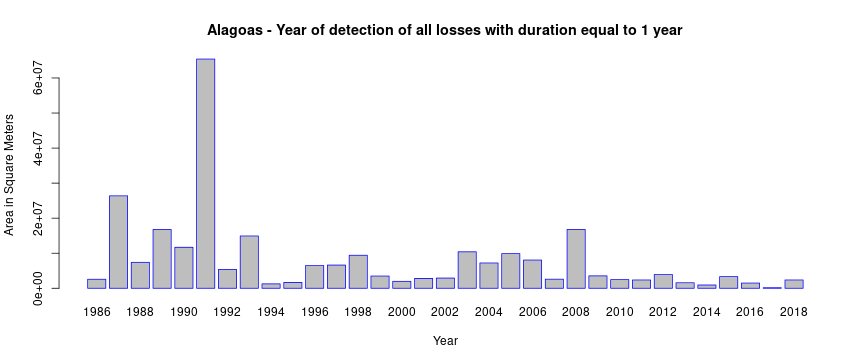
\includegraphics[scale=.5]{images/loss_graphics/Alagoas_loss_eq1.png}
    \caption{Perda de área por ano em Alagoas}
    \label{fig:loss_alagoas}
\end{figure}

\begin{figure}[H]
    \centering
    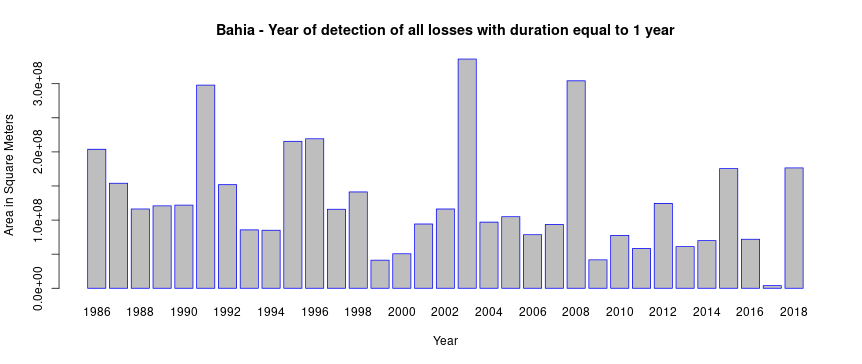
\includegraphics[scale=.5]{images/loss_graphics/Bahia_loss_eq1.png}
    \caption{Perda de área por ano na Bahia}
    \label{fig:loss_bahia}
\end{figure}

\begin{figure}[H]
    \centering
    \includegraphics[scale=.5]{images/loss_graphics/Espírito Santo_loss_eq1.png}
    \caption{Perda de área por ano no Espírito Santo}
    \label{fig:loss_espirito_santo}
\end{figure}

\begin{figure}[H]
    \centering
    \includegraphics[scale=.5]{images/loss_graphics/Goiás_loss_eq1.png}
    \caption{Perda de área por ano em Goiás}
    \label{fig:loss_goias}
\end{figure}

\begin{figure}[H]
    \centering
    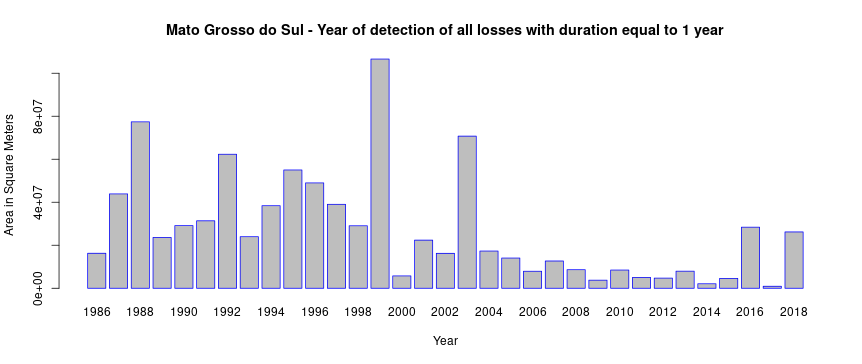
\includegraphics[scale=.5]{images/loss_graphics/Mato Grosso do Sul_loss_eq1.png}
    \caption{Perda de área por ano no Mato Grosso do Sul}
    \label{fig:loss_mato_grosso_sul}
\end{figure}

\begin{figure}[H]
    \centering
    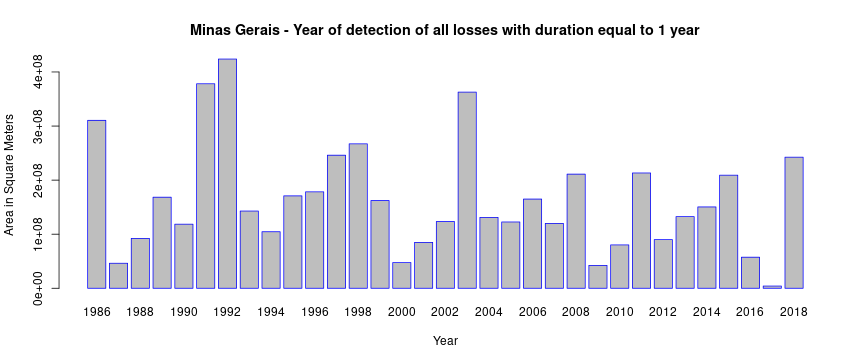
\includegraphics[scale=.5]{images/loss_graphics/Minas Gerais_loss_eq1.png}
    \caption{Perda de área por ano em Minas Gerais}
    \label{fig:loss_minas_gerais}
\end{figure}

\begin{figure}[H]
    \centering
    \includegraphics[scale=.5]{images/loss_graphics/Paraíba_loss_eq1.png}
    \caption{Perda de área por ano na Paraíba}
    \label{fig:loss_paraiba}
\end{figure}

\begin{figure}[H]
    \centering
    \includegraphics[scale=.5]{images/loss_graphics/Paraná_loss_eq1.png}
    \caption{Perda de área por ano no Paraná}
    \label{fig:loss_parana}
\end{figure}

\begin{figure}[H]
    \centering
    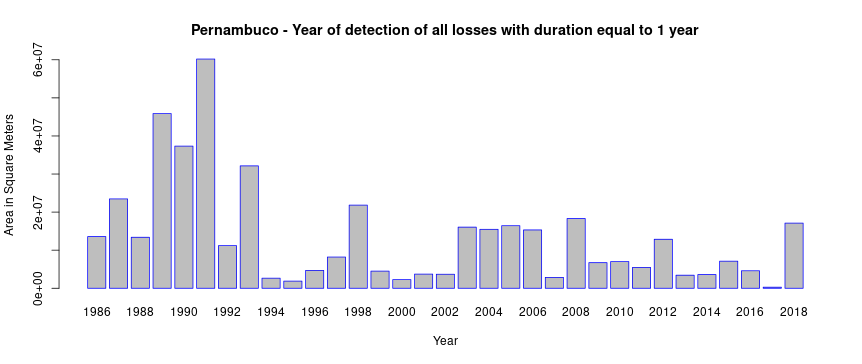
\includegraphics[scale=.5]{images/loss_graphics/Pernambuco_loss_eq1.png}
    \caption{Perda de área por ano em Pernambuco}
    \label{fig:loss_pernambuco}
\end{figure}

\begin{figure}[H]
    \centering
    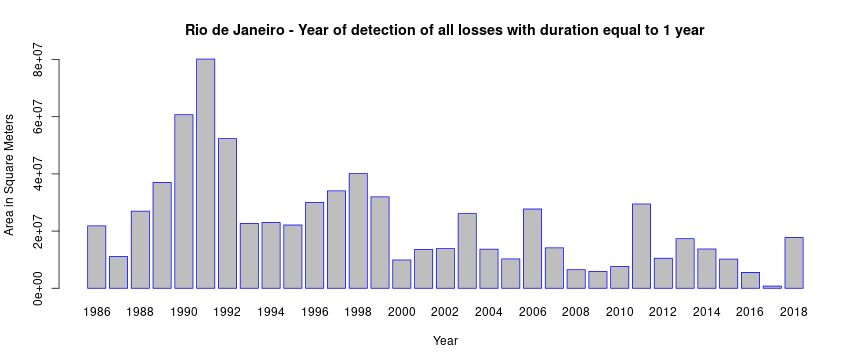
\includegraphics[scale=.5]{images/loss_graphics/Rio de Janeiro_loss_eq1.png}
    \caption{Perda de área por ano no Rio de Janeiro}
    \label{fig:loss_rio_de_janeiro}
\end{figure}

\begin{figure}[H]
    \centering
    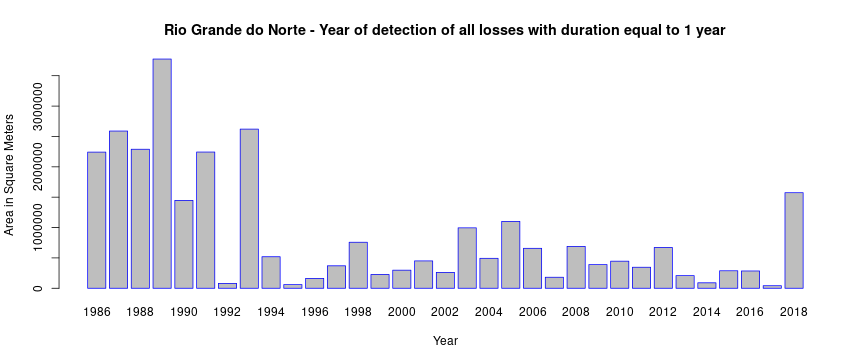
\includegraphics[scale=.5]{images/loss_graphics/Rio Grande do Norte_loss_eq1.png}
    \caption{Perda de área por ano no Rio Grande do Norte}
    \label{fig:loss_rio_grande_do_norte}
\end{figure}

\begin{figure}[H]
    \centering
    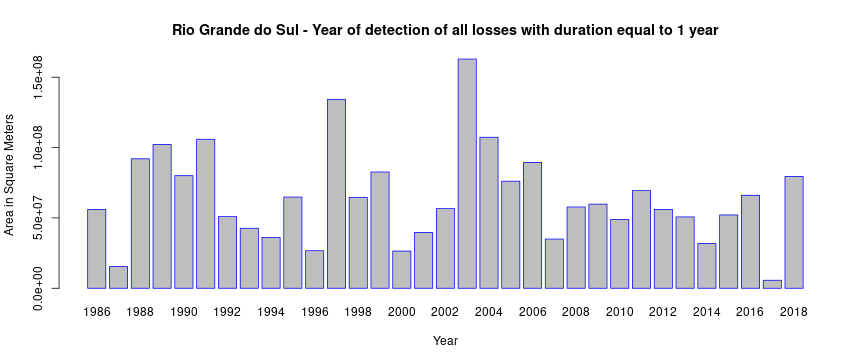
\includegraphics[scale=.5]{images/loss_graphics/Rio Grande do Sul_loss_eq1.png}
    \caption{Perda de área por ano no Rio Grande do Sul}
    \label{fig:loss_rio_grande_do_sul}
\end{figure}

\begin{figure}[H]
    \centering
    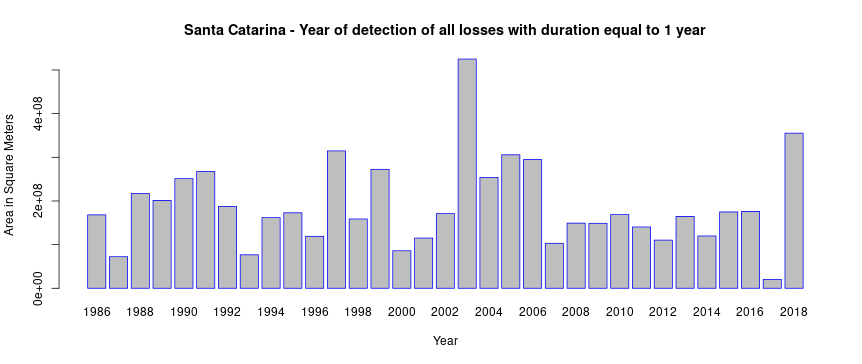
\includegraphics[scale=.5]{images/loss_graphics/Santa Catarina_loss_eq1.png}
    \caption{Perda de área por ano em Santa Catarina}
    \label{fig:loss_santa_catarina}
\end{figure}

\begin{figure}[H]
    \centering
    \includegraphics[scale=.5]{images/loss_graphics/São Paulo_loss_eq1.png}
    \caption{Perda de área por ano em São Paulo}
    \label{fig:loss_sao_paulo}
\end{figure}

\begin{figure}[H]
    \centering
    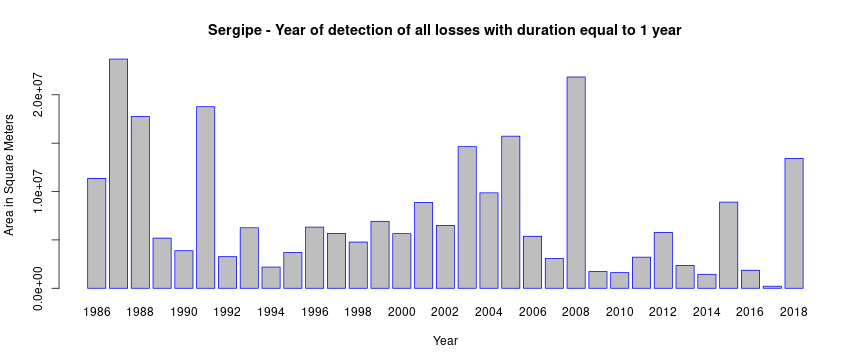
\includegraphics[scale=.5]{images/loss_graphics/Sergipe_loss_eq1.png}
    \caption{Perda de área por ano em Sergipe}
    \label{fig:loss_sergipe}
\end{figure}

\end{appendices}

\newpage
\section{Apêndice - Total de área ganha ano a ano por estado}

\begin{figure}[H]
    \centering
    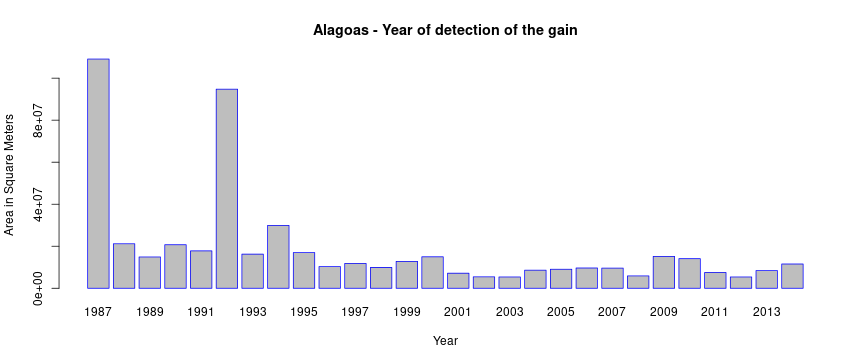
\includegraphics[scale=.5]{images/gain_graphics/Alagoas_gain.png}
    \caption{Ganho de área por ano em Alagoas}
    \label{fig:gain_alagoas}
\end{figure}

\begin{figure}[H]
    \centering
    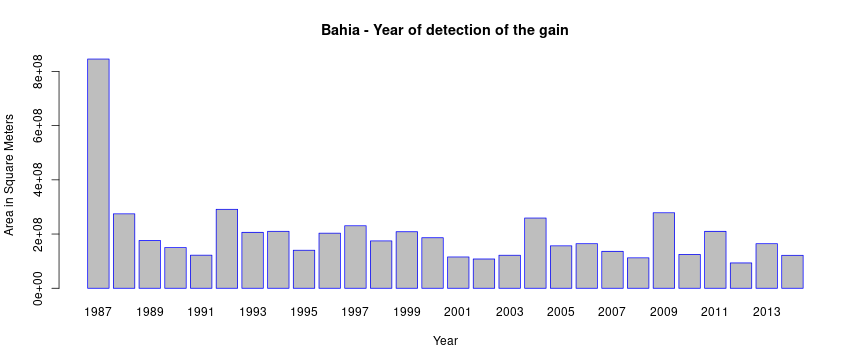
\includegraphics[scale=.5]{images/gain_graphics/Bahia_gain.png}
    \caption{Ganho de área por ano na Bahia}
    \label{fig:gain_bahia}
\end{figure}

\begin{figure}[H]
    \centering
    \includegraphics[scale=.5]{images/gain_graphics/Espírito Santo_gain.png}
    \caption{Ganho de área por ano no Espírito Santo}
    \label{fig:gain_espirito_santo}
\end{figure}

\begin{figure}[H]
    \centering
    \includegraphics[scale=.5]{images/gain_graphics/Goiás_gain.png}
    \caption{Ganho de área por ano em Goiás}
    \label{fig:gain_goias}
\end{figure}

\begin{figure}[H]
    \centering
    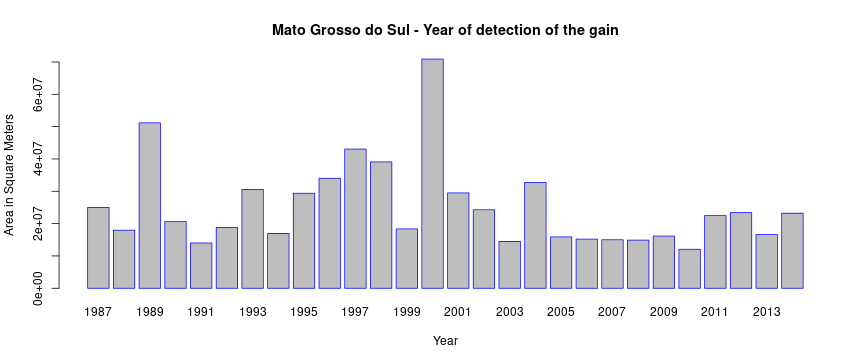
\includegraphics[scale=.5]{images/gain_graphics/Mato Grosso do Sul_gain.png}
    \caption{Ganho de área por ano no Mato Grosso do Sul}
    \label{fig:gain_mato_grosso_sul}
\end{figure}

\begin{figure}[H]
    \centering
    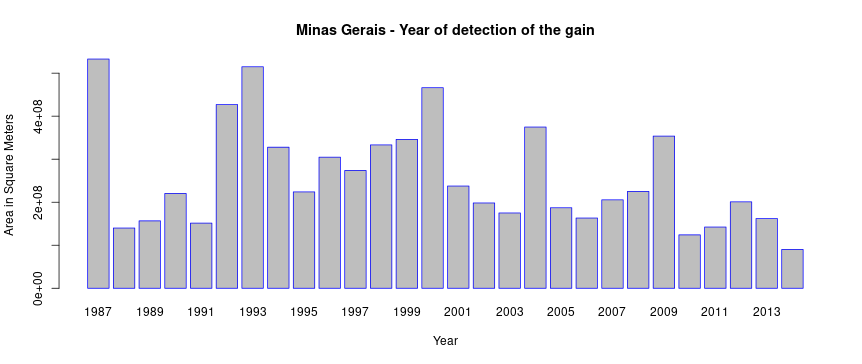
\includegraphics[scale=.5]{images/gain_graphics/Minas Gerais_gain.png}
    \caption{Ganho de área por ano em Minas Gerais}
    \label{fig:gain_minas_gerais}
\end{figure}

\begin{figure}[H]
    \centering
    \includegraphics[scale=.5]{images/gain_graphics/Paraíba_gain.png}
    \caption{Ganho de área por ano na Paraíba}
    \label{fig:gain_paraiba}
\end{figure}

\begin{figure}[H]
    \centering
    \includegraphics[scale=.5]{images/gain_graphics/Paraná_gain.png}
    \caption{Ganho de área por ano no Paraná}
    \label{fig:gain_parana}
\end{figure}

\begin{figure}[H]
    \centering
    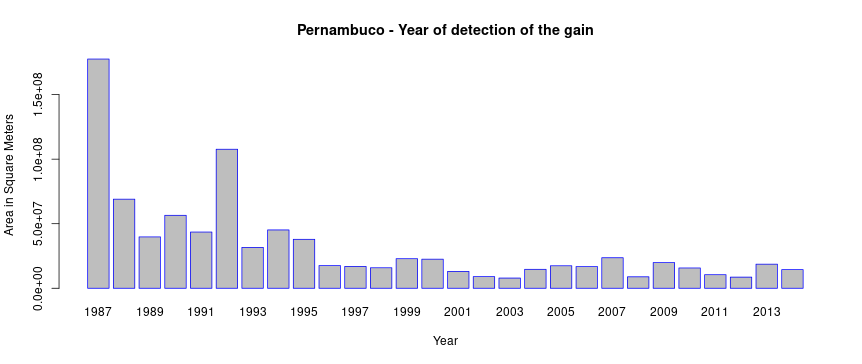
\includegraphics[scale=.5]{images/gain_graphics/Pernambuco_gain.png}
    \caption{Ganho de área por ano em Pernambuco}
    \label{fig:gain_pernambuco}
\end{figure}

\begin{figure}[H]
    \centering
    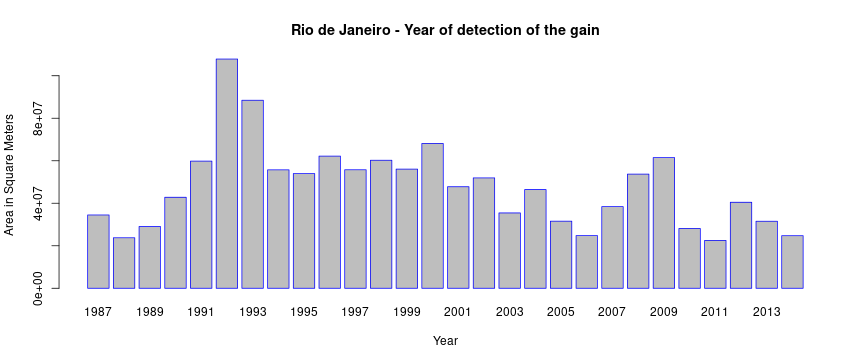
\includegraphics[scale=.5]{images/gain_graphics/Rio de Janeiro_gain.png}
    \caption{Ganho de área por ano no Rio de Janeiro}
    \label{fig:gain_rio_de_janeiro}
\end{figure}

\begin{figure}[H]
    \centering
    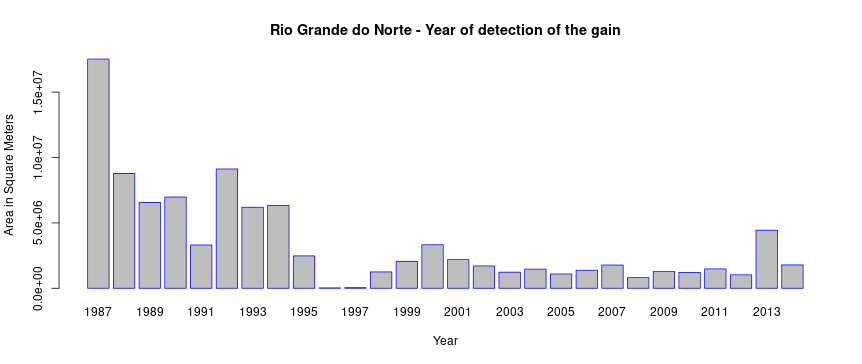
\includegraphics[scale=.5]{images/gain_graphics/Rio Grande do Norte_gain.png}
    \caption{Ganho de área por ano no Rio Grande do Norte}
    \label{fig:gain_rio_grande_do_norte}
\end{figure}

\begin{figure}[H]
    \centering
    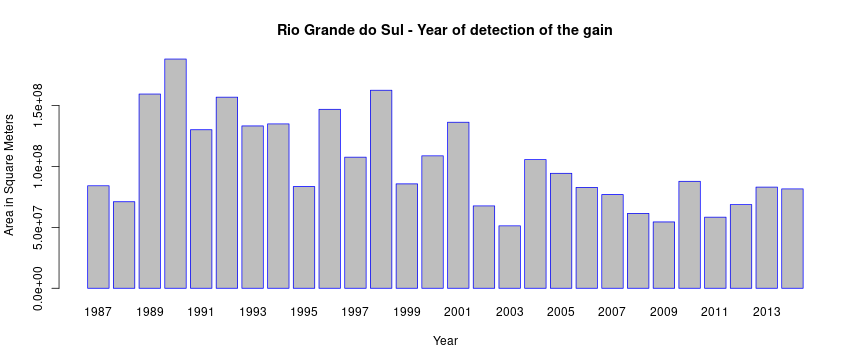
\includegraphics[scale=.5]{images/gain_graphics/Rio Grande do Sul_gain.png}
    \caption{Ganho de área por ano no Rio Grande do Sul}
    \label{fig:gain_rio_grande_do_sul}
\end{figure}

\begin{figure}[H]
    \centering
    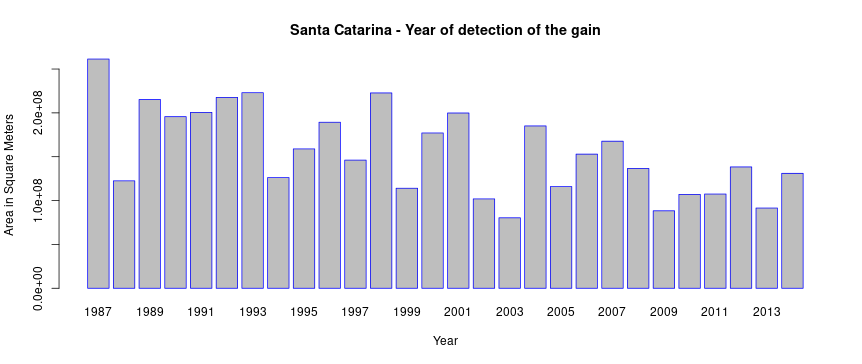
\includegraphics[scale=.5]{images/gain_graphics/Santa Catarina_gain.png}
    \caption{Ganho de área por ano em Santa Catarina}
    \label{fig:gain_santa_catarina}
\end{figure}

\begin{figure}[H]
    \centering
    \includegraphics[scale=.5]{images/gain_graphics/São Paulo_gain.png}
    \caption{Ganho de área por ano em São Paulo}
    \label{fig:gain_sao_paulo}
\end{figure}

\begin{figure}[H]
    \centering
    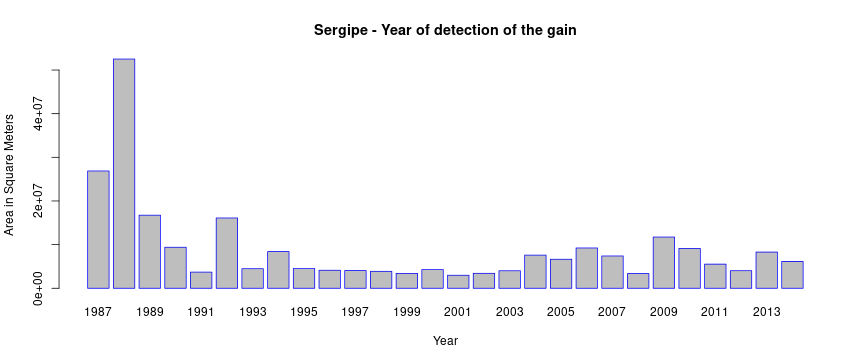
\includegraphics[scale=.5]{images/gain_graphics/Sergipe_gain.png}
    \caption{Ganho de área por ano em Sergipe}
    \label{fig:gain_sergipe}
\end{figure}

\end{document}